\documentclass[12pt]{n-te}
\usepackage{caption}
\usepackage[utf8]{inputenc}
\usepackage{
  graphicx,
  wasysym
}

\ifpdf
\usepackage{pdfpages}
\usepackage[absolute]{textpos}
\usepackage{graphicx} 
\fi

\usepackage{amssymb}

\nedition{1}{WS 2011/2012}

%% Trennregeln
\hyphenation{
  AStA
  Mit-be-wohnerIn-nen
  Pro-fessorInnen
  erwischt
  viiieel
  y-Nummer
  Uniaccount
}
\usepackage{multicol}

% Könnte man demmächst verwenden, wird aber derzeit wohl noch nicht verwendet, sondern vor ort jeweils lang und breit gemacht:
\newcommand{\nsection}[1]{\end{multicols}\section{#1}\begin{multicols}{2}}

\newcommand{\mehrInfo}[1]{\fbox{$\rightarrow$ #1 }}
%Hauptdokument der Erstsemesterzeitschrift "Erste" der Fachgruppe Informatik
%\documentclass[
%	final,%hide anything from todonotes	
%%	]{scrartcl}
%	nexus,
%	twoside
%	]{tubsartcl}

\documentclass[
  final,
  a4paper,              % DIN A4
  style=screen,
  twoside,
  nexus,                % corporate design font
]{tubsartcl}


\usepackage[utf8]{inputenc}
\usepackage{graphicx}
\usepackage{amssymb}
\usepackage[T1]{fontenc}
\usepackage{multicol}
\usepackage{comment}
\usepackage[ngerman]{babel}
\usepackage{wrapfig}
\usepackage[babel,german=quotes]{csquotes}
\usepackage{todonotes}
\usepackage{etoolbox}
\usepackage{sectsty}
\renewcommand{\familydefault}{\sfdefault}

%\clubpenalty = 10000
%\widowpenalty = 10000 
%\displaywidowpenalty = 10000

% Trennregeln
\hyphenation{
	AStA
	Mit-be-wohnerIn-nen
	Pro-fessorInnen
	erwischt
	viiieel
	y-Nummer
	Uniaccount
}

% left aligned sections
%\allsectionsfont{\raggedright}


\settoggle{winter}{true}
\setcounter{version}{6}


\KOMAoptions{twoside, headsepline}

\geometry{margin=1.5cm}
\geometry{twoside}
%\geometry{bindingoffset=7mm}
\geometry{includehead} 
\geometry{includefoot}
\geometry{footnotesep=2em}
\geometry{footskip=\footskip-2em}

%layout-experimente
\setlength{\columnsep}{20pt}
\pagestyle{headings}



% Toggles between winter term and summer term 
\newtoggle{winter}

% This system is meant to make updating the Erste for the new semster simple. Every semster gets a new version number that is larger than the previous one (assigned in config.tex). 
% By using \tocheck, defined below, todos can be left in the source and disabled one by one by incresing the version number of the tocheck. Once all todos are adressed, the new version can be released. Later all todos can be enabled again by incrementing the version number.
\newcounter{version}

% Defines a conditional todo. 2 mandatory arguments:
% 1st param, Valid to version: This todo has been adressd as of the given version
% 2nd param, Todo description: What needs to be done to adress this todo
\newrobustcmd{\tocheck}[2]{
	\ifnumless{#1}{\value{version}}{
		\todo[inline]{#2}
	}{}
}

% Versioned url. 2 mandatory arguments:
% 1st param, Valid to version: This url is still valid as of version
% 2nd param, URL: The url
\newrobustcmd{\verUrl}[2]{\ifnumless{#1}{\value{version}}{\todo[inline]{Check \url{#2}}}{}\url{#2}}
\newrobustcmd{\verHref}[4][]{\ifnumless{#2}{\value{version}}{\todo[inline]{Check \url{#3}}}{}\href[#1]{#3}{\nolinkurl{#4}}}

\newrobustcmd{\FginfoUrl}[0]{https://fginfo.tu-braunschweig.de}
\newrobustcmd{\fginfoUrl}[0]{\verUrl{8}{https://fginfo.tu-braunschweig.de}}

%%

\newrobustcmd{\xkcd}[2]{
	\begin{center}
		\includegraphics[#1]{bilder/XKCD/#2}
	\end{center}
}


% creates a blank page

\newcommand{\blankpage}{
	\newpage
	\thispagestyle{empty}
	\mbox{}
	\newpage
}


% creates a stundenplan
\newenvironment{stundenplan}[6]{%
	\newcommand{\wTag}{#1/6}%
	\newcommand{\hPlan}{#2}%
	\newcommand{\hAbendHeader}{.5}%
	\newcommand{\hAbend}{1.6}%
	\newcommand{\tStart}{zeit(#3,#4)}%
	\newcommand{\tEnde}{zeit(#5,#6)}%

	\pgfmathdeclarefunction{zeit}{2}{\pgfmathparse{##1 + ##2 / 60}}%
	\pgfmathdeclarefunction{tmpYZeit}{1}{\pgfmathparse{-\hPlan * (##1-\tStart) / (\tEnde-\tStart)}}%
	\pgfmathdeclarefunction{yZeit}{1}{\pgfmathparse{%
		max(min(tmpYZeit(##1), tmpYZeit(\tStart)), tmpYZeit(\tEnde)-\hAbendHeader-\hAbend)%
	}}%

%
	\tikzset{%
	  termin/.style={%
	   anchor=north west,%
	   align=left,%
	   %execute at begin node=\setlength{\baselineskip}{1.2em}%
	  }%
	}%

	\newcommand{\tNode}[2]{%
		\node [termin] at (TERMIN) {%
			\begin{varwidth}{1cm*\wTag - .2cm}%
			##1\\%
			\scriptsize ##2%
			\end{varwidth}%
		};%
	}%

%
	\newcommand{\Termin}[8]{%
		%1: Beschreibung, 2: Ort, 3: Tag, 4: Start Stunde, 5: Start Minute, 6: Ende Stunde, 7: Ende Minute, 8: Farbe %
		\draw [##8](\wTag * ##3,{yZeit(zeit(##4,##5))}) coordinate (TERMIN) rectangle (##3  * \wTag + \wTag,{yZeit(zeit(##6,##7))});%
		\tNode{##1}{##2}%
	}%

	\newcommand{\termin}[8]{%
		%1: Beschreibung, 2: Ort, 3: Tag, 4: Start Stunde, 5: Start Minute, 6: Ende Stunde, 7: Ende Minute, 8: Farbe (Fügt Zeit automatisch in Beschreibung ein)%
		\Termin{##1}{##4:##5 -- ##6:##7\ifstrempty{##2}{}{, ##2}}{##3}{##4}{##5}{##6}{##7}{##8}%
	}%

	\newcommand{\abendtermin}[4]{%
		%1: Beschreibung, 2: Ort, 3: Tag, 4: Farbe%
		\draw [##4](\wTag * ##3,-\hPlan-\hAbendHeader) coordinate (TERMIN) rectangle (##3  * \wTag + \wTag, -\hPlan-\hAbendHeader-\hAbend);%
		\tNode{##1}{##2}%
	}%
	\begin{tikzpicture}[font=\small]%
	% spalten
	\foreach \x in {0,...,5}{
		\draw (\x*\wTag,0) -- (\x*\wTag,-\hPlan);
		\draw (\x*\wTag,-\hPlan-\hAbendHeader) -- (\x*\wTag,-\hPlan-\hAbendHeader-\hAbend);
	}
	\draw (6*\wTag,0) -- (6*\wTag,-\hPlan-\hAbendHeader-\hAbend);

	\draw (0,0)--(6*\wTag,0);
	\draw (0, -\hPlan) coordinate (ABEND) rectangle (5*\wTag, -\hPlan-\hAbendHeader);
	\node [anchor=north west,align=center,minimum width=5cm*\wTag] at (ABEND) {\scriptsize \emph{Abend}};
	\draw (0, -\hPlan-\hAbendHeader-\hAbend)--(6*\wTag, -\hPlan-\hAbendHeader-\hAbend);

	\node [anchor=south] at (.5* \wTag,0) {\textbf{Montag}};
	\node [anchor=south] at (1.5* \wTag,0) {\textbf{Dienstag}};
	\node [anchor=south] at (2.5* \wTag,0) {\textbf{Mittwoch\vphantom{g}}};
	\node [anchor=south] at (3.5* \wTag,0) {\textbf{Donnerstag}};
	\node [anchor=south] at (4.5* \wTag,0) {\textbf{Freitag}};
	\node [anchor=south] at (5.5* \wTag,0) {\textbf{Wochenende\vphantom{g}}};
}{\end{tikzpicture}}


\settoggle{winter}{true}
\setcounter{version}{6}

\begin{document}
	\thispagestyle{empty}

	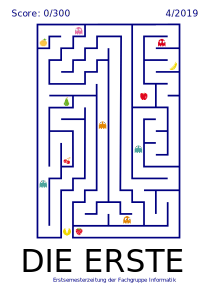
\includepdf[pages={1}]{bilder/Erste_Cover/cover.pdf}

	\listoftodos
	\vspace*{2.5cm}
	\xkcd{width=0.9\textwidth}{tech_support_cheat_sheet}

	\newpage

	\setcounter{page}{1}
	\tableofcontents

	\vfill
	\xkcd{width=\textwidth}{sail}

	\newpage

	
\section{Vorwort}
\label{vorwort}
	\begin{multicols}{2}
	\subsection*{Willkommen in der Informatik!}	

	Ein neues Semester hat begonnen und wieder strömen unzählige neue Gesichter auf den Campus um das Abenteuer Studium zu beginnen oder fortzusetzen. Da das nicht immer ganz einfach ist haben wir, die Fachgruppe Informatik für die Erstsemester unserer Fachrichtung einen kleinen Leitfaden zusammengestellt - die 1-te.

	Auf den folgenden Seiten werden wir hoffentlich einige der typischen Fragen beantworten, die einen am Anfang des Studiums quälen. Außerdem möchten wir natürlich uns, die Fachgruppe vorstellen (s. Seite \pageref{fachgruppe}) und eventuell noch die ein oder andere hilfreiche Information mitgeben. 

	\subsubsection*{Aufbau dieses Heftes}
		In der ersten Hälfte dieses Heftes sind wichtige
		Erklärungen zum Studienbeginn, dem Studiengang und der
		universitären Infrastruktur. Weitere Informationen zu
		uns und unserer Gremienarbeit, sowie weitere
		Informationen sind in der zweiten Hälfte.
\columnbreak
	\subsubsection*{Die Fachgruppe Online}
		Natürlich gibt es uns auch online - auf der Seite \url{http://fginfo.cs.tu-bs.de}. Beispielsweise stehen dort aktuelle Termine wie Spiele- oder Grillabende. Auch gibt es dort noch einmal die Inhalte dieses Heftes, samt den Aktualisierungen die erst nach dem Druck bekannt wurden. 

	\vspace*{0.5cm}

	Viel Spaß und Erfolg im  Studium wünscht  die\\
	\hspace*{2cm}Fachgruppe Informatik
	\end{multicols}
	\vspace{0.5cm}
	\begin{center} 
\includegraphics[totalheight=12cm]{bilder/XKCD/dorm_poster}
\end{center}


	\vfill
	\xkcd{width=.7\textwidth}{dorm_poster}

	\newpage

	\section{Die ersten Tage}
		% !TEX root = ../../1-te.tex

\subsection{Checkliste}
\label{checkliste}
	Hier wird zusammengefasst, was du in den ersten Tagen des Studiums unbedingt erledigen solltest. Wenn du die ToDos auf der Checkliste nach Erledigung abhakst, verlierst du nicht den Überblick und vergisst nichts.
	
\vspace*{0.5cm}
% !TEX root = ../../1-te.tex

\begin{center}
\begin{tabular}{|p{3mm}|l|p{8cm}|c|c|}
\hline \checkmark 
       & \textbf{Todo}             & \textbf{Zu erledigen bis}                                  & \textbf{Seite}               & \textbf{Muss?} \\ 
\hline & BAföG beantragen          & Spätestens Ende \iftoggle{winter}{Oktober}{April}          & \pageref{todobafoeg}         & optional \\ 
\hline & Wohnsitz ummelden         & 1 Woche nach Umzug                                         & \pageref{todoummelden}       & ja \\
\hline & Mailinglisten             & So früh wie möglich                                        & \pageref{mailinglisten}      & ja \\ 
\hline & Studiengrobplanung        & Vor dem Stundenplan bauen                                  & \pageref{grob}               & ja \\
\hline & Auflagen klären           & So früh wie möglich, final: Ende 2. Semester               & \pageref{auflagen}           & nur Master \\ 
\hline & Persönlicher Stundenplan  & Siehe Terminzettel der Fachgruppe                          & \pageref{masterstundenplan}  & ja \\ 
\hline & Prüfungsbogen             & Spätestens \iftoggle{winter}{Dezember}{Mai}                & \pageref{todoanmeldung}      & ja \\ 
\hline & Prüfungsanmeldung         & 12.12.2017 - 11.01.2018, schriftlich oder online           & \pageref{todoanmeldung}      & ja \\ 
\hline & Blog abonnieren           & So früh wie möglich                                        & \pageref{fachgruppe}         & ja \\ 
\hline & Prüfungsordnung lesen     & Zu den ersten Klausuren                                    & \pageref{po}                 & ja \\ 
\hline & TUcard validieren         & Zu Beginn und zu jedem neuen Semester                      & \pageref{tucard}             & ja \\
\hline & Bibliotheksausweis        & Vor der ersten Buchausleihe                                & \pageref{todobib}            & optional \\
\hline & Stud.IP-Nachrichten weiterleiten  & Wenn man nichts verpassen möchte         & \pageref{tumails}            & optional \\
\hline
\end{tabular} 
\end{center}
\tocheck{4}{Exakte Daten Anmeldewoche einfügen, s.\url{https://www.tu-braunschweig.de/fk1/service/informatik/pa}}

\begin{multicols}{2}

\subsubsection{BAföG}
	\label{todobafoeg}

	Wer Studierendenförderung nach dem Bundesausbildungsförderungsgesetz (BAföG) beantragen möchte, sollte sich am besten gründlich informieren. Sehr zu empfehlen ist da: \\
	\verUrl{4}{https://www.xn--bafg-7qa.de/}
 
	Förderungsanträge gibt es zum Download oder in Papierform im EG des Amtes für Ausbildungsförderung in der Wilhelmstraße 1. Wenn du BAföG beantragen möchtest, stelle den Antrag so früh wie möglich, denn es wird nicht rückwirkend gezahlt.

	Zum Anfang des Semester ist mit längeren Wartezeiten zu rechnen, im Notfall kannst du beim AStA-Sozialreferat ein kurzfristiges, zinsloses Darlehen beantragen, um den ersten Monat zu überbrücken. Das Darlehen ist auf 450 Euro begrenzt und muss spätestens nach drei Monaten zurückgezahlt werden. Mehr Informationen findest du auf der Seite des Sozialreferats: \verUrl{4}{https://www.asta.tu-braunschweig.de/referate/sozialreferat/}


\subsubsection{Ummelden}
	\label{todoummelden}

	Wer neu nach Braunschweig gezogen ist, muss sich innerhalb einer Woche beim Einwohnermeldeamt anmelden. Wenn ihr die Frist verpasst, drohen theoretisch Strafen, aber praktisch sieht es da nicht so streng aus. Wenn man Braunschweig als Erstwohnsitz wählt, bekommt man (ein Jahr später) eine einmalige Zuzugsprämie von 100 Euro (Immatrikulationsbescheinigung nicht vergessen). Alternativ kann man Braunschweig auch als Zweitwohnsitz wählen.

\subsubsection{Prüfungsanmeldung}
	\label{todoanmeldung}

	Du musst dich für alle Prüfungen, an denen du teilnehmen willst, vorher beim Prüfungsamt anmelden. Die Fristen sind relativ früh im Semester. Die Termine werden im Laufe des Semesters veröffentlicht (Seiten des P-Amtes (\verUrl{3}{https://www.tu-braunschweig.de/fk1/service/informatik/pa}), Mailingliste). Prüfungen können im Prüfungsanmeldezeitraum schriftlich im Prüfungsamt oder online über das QIS-Portal angemeldet werden.
	Vor deiner ersten Prüfungsanmeldung musst du außerdem ein Datenblatt ausfüllen. Es empfiehlt sich, das bereits vor der Anmeldewoche zu machen, weil die Schlangen dann nicht so lang sind.

	Für die Online-Anmeldung benötigst du eine TAN-Liste, die du dir vorher im Prüfungsamt organisieren musst.

	Unter folgendem Link findest du außerdem alle Prüfungstermine für die Informatik:
	\verUrl{3}{https://www.tu-braunschweig.de/fk1/service/informatik/pa}

\subsubsection{TUcard}
	\label{tucard}
	
	Alle Studierenden der TU erhaten den elektronische Studierendenausweis TUcard, die auch als Bibliotheksausweis und Mensakarte genutzt werden kann.

	Damit die Karte gültig ist, muss sie zu Beginn und zu jedem neuen Semester validiert werden. Das bedeutet, dass der Thermostreifen auf der Karte in einem Validierungsdrucker mit den aktuellen Daten beschrieben wird.

	Das Börsenguthaben der Karte, beispielsweise zum Bezahlen in der Mensa, kann an Börsenaufwertern (auch denen, die sich bereits in den Mensen befinden) aufgeladen werden.

	Zum Drucken kann Guthaben der Karte auf ein Druckkonto umgebucht werden. Dies geschieht an den Druckkontenumbuchern.

	Weitere Informationen zur TUcard findest du unter: \verUrl{3}{https://www.tu-braunschweig.de/studium/imstudium/tucard}

\subsubsection{Uni-Bibliothek}
	\label{todobib}

	Um Bücher in der Uni-Bibliothek ausleihen zu können, brauchst du einen Ausweis. Dieser ist in deiner TUcard integriert. Diesen kannst du an einem der Terminals in der Bibliothek, oder online beantragen und am Schalter freischalten. Je nachdem, ob du zu Beginn schon Bücher brauchst, kannst du die Karte auch später aktivieren.

	In der Bibliothek stehen außerdem Kopierer bereit, die du nutzen kannst. Einen davon kannst du mit Kleingeld befüllen, kompfortabler geht es aber mit einer Kopierkarte. Die bekommst du für ein paar Euro direkt in der Bibliothek. Zu Semesterbeginn gibt es oft noch Einführungskurse in die Bibliotheksbenutzung. Ob du deinen Bibliotheksausweis vor oder nach diesem Kurs aktivierst, ist egal.
	
\end{multicols}

		% !TEX root = ../../1-te.tex

\subsection{Wichtige Termine am Anfang des Studiums}

\tocheck{2}{Termine für aktuelle O-Woche einfügen}

Zu Beginn des Semesters wird es Begrüßungs- und Einführungsveranstaltungen geben. Wir möchten den Start an der TU Braunschweig so gut wie möglich begleiten. Bis zum Semesterstart können sich einzelnen Termine noch ändern, den ganz aktuellen Stand gibt es online unter \verUrl{2}{http://fginfo.cs.tu-bs.de/index.php/ersti-infos/}.

\renewcommand{\labelitemi}{$\bullet$}
\renewcommand{\labelitemii}{$\bullet$}
\renewcommand{\labelitemiii}{$\bullet$}
\renewcommand{\labelitemiv}{$\bullet$}

\begin{itemize}
	\item Vorkurs: 03. – 12. Oktober 2016
	
	\item Donnerstag 13. Oktober
	\begin{itemize}
		\item Ab 15:00 Uhr Linux Install Party im Informatikzentrum, Raum IZ 150
		\item Im Anschluss Grillen (ca. 18:00), \textbf{Grillgut bringt jeder selbst mit}
	\end{itemize}

	\item Montag, 17. Oktober 2016
	\begin{itemize}
		\item 09:30 Uhr: Begrüßung durch die Fakultät: PK 2.2
	\end{itemize}

	\item Vorlesungsbeginn: Montag, 17. Oktober 2016

	\item Einführungswoche für Erstsemester:
	\begin{itemize}
		\item Dienstag, 18. Oktober
		\begin{itemize}
			\item 09:30 Uhr: gemeinsames Frühstück auf der IZ Plaza im 1. Obergeschoss. \textbf{Besteck bringt jeder selber mit}
			\item 11:30 erste Vorlesung Lineare Algebra
			\item ab ca. 13:30: Begrüßung durch FG Informatik \& Vortrag zur Studien- und Stundenplan-Planung
			\item Im Anschluss (ca. 12:30 Uhr): Campusführung inklusive Mittagspause in der Mensa :)
			\item 19:00 Kneipentour (Treffpunkt vor dem Haupteingang der Mensa)
		\end{itemize}

		\item Mittwoch, 19. Oktober
		\begin{itemize}
			\item 10:00 - 18:00 Uhr Studium Generale
		\end{itemize}

		\item Donnerstag, 20. Oktober
		\begin{itemize}
			\item 13:00 Uhr: Real-Life Scotland Yard (Treffpunkt auf dem Platz zwischen dem Audimax und der Uni-Bibliothek)
			\item Anschließend Siegerehrung im Informatikzentrum (IZ 150).
			\item Ab 18:30 Uhr: analoger Spieleabend der Informatik vor dem Fachgruppenraum (IZ 150)
		\end{itemize}
	\end{itemize}

	\item Ersti-Wochenende:
	\begin{itemize}
		\item Wann? \emph{21. - 23. Oktober 2016}
		\item Wo? \emph{Naturfreundehaus Eichsfelder Hütte (St. Andreasberg)}
		\item Was? Lerne deine Mitstudierenden kennen, habe Spaß :)
		\item Finanzierung? Größtenteils aus Studienqualitätsmitteln, dazu \emph{10 Euro Selbstkostenbeitrag}
		\item Fristen: \emph{Anmeldung bis 18. Oktober 2016, Bezahlung des Selbstkostenbeitrags ebenfalls bis 18. Oktober 2016}
		\item Weitere Informationen findet ihr in unserem Info-Schreiben zur Ersti-Fahrt (\verUrl{2}{https://fginfo.cs.tu-bs.de/wp342/wp-content/uploads/2016/09/Ersti-Fahrt-Info-WS1617.pdf})
		\item Den Anmeldebogen findet ihr unter \verUrl{2}{https://fginfo.cs.tu-bs.de/wp342/wp-content/uploads/2016/09/Anmeldung-Ersti-Fahrt-WS1617.pdf}
	\end{itemize}
\end{itemize}

		\vfill
		\xkcd{totalheight=6cm}{computer_problems}
		\vfill
	\newpage

	\section{Studienplan(ung) für jeden}
		\label{studienplan}
		\begin{multicols}{2}
		\subsection{Verantwortung}
	\textit{Große Macht bringt große Verantwortung mit sich!}, sagte schon Ben Parker, der Onkel von Spiderman. Das heißt für dich: Du hast die Macht und die Verantwortung über deinen Studienfortgang. Das beginnt bei der Entscheidung, überhaupt zu studieren, die Wahl des Faches und der Universität und erstreckt sich über die Wahl, welche Fächer du hörst und wann du das tust, bis hin zur Einflussnahme auf den gesamten Studiengang.

	Es besteht aber auch die Möglichkeit diese Verantwortung abzugeben. Es gibt einen Studienplan, der dir vorschlägt, wie du deine Fächer wählen und anordnen kannst, um in Regelstudienzeit fertig zu werden. Für den Bachelor sieht dieser Plan sehr konkret aus, für den Master ist er abstrakter gehalten, aber deckt immer noch nur partiell die Wahlmöglichkeiten ab. Das kann und soll er auch nicht -- es handelt sich um zwei von unendlich vielen Möglichkeiten, zum Studienabschluss zu kommen. % Verantwortung
		\subsection{Zwei Studiengänge unter einem Hut}
	Seit der Bologna-Reform gibt es an der TU Braunschweig zwei Studiengänge - \textit{Bachelor und Master}. Viele Informationen über das Studium betreffen beide, deshalb ist diese Zeitung für alle Erstsemester. Nach der allgemeinen Einleitung folgen die speziellen Abschnitte für Bachelor- (ab S. \pageref{bachelor}) und Master-Ersties (ab Seite \pageref{master}).

\subsubsection{Herden, Rudel und Einzelgänger}
	Bevor es in die Untiefen der Prüfungsordnungen und formalen Anforderungen geht, ein paar Worte zu einem sozialen Phänomen. Der recht feste Stundenplan im Bachelor-Studium sorgt dafür, dass man dort in der Regel mit vielen Mitstudierenden zusammensitzt, die in der gleichen Situation sind wie man selbst: Neu hier und mit den gleichen Fragen und Sorgen. Und ist ein Block zu Ende, so zieht man gemeinsam zum nächsten Raum, wo man mit praktisch der gleichen Gruppe das nächste Fach abgrast. Eine typische Herde also.

	Im Master ist das grundlegend anders. Jeder hört andere Vorlesungen, und in den \emph{Mastervorlesungen} tummeln sich nicht nur Masterstudierende, sondern auch Bachelor- und Diplom- oder gar fachverwandte Studierende, wie z.B. Wirtschaftsinformatik. Da kann es eine ganze Weile dauern, bis man weiß, wer auch im Masterstudium ist und gegebenfalls auch noch im gleichen Jahrgang. Selbst dann haben diese Leute ihren Bachelor hier oder dort, in diesem oder jenem Fach an einer Uni oder FH gemacht. Vielleicht haben die neben dir zuvor ganz andere Dinge gelernt, vielleicht sind sie hier um sich auf etwas komplett anderes zu spezialisieren als du.

	Keine Frage: Diese Mischung macht es spannender, bunter und vielseitiger, aber auf jeden Fall auch schwieriger. Wir können hier kaum Tipps geben, wie man als Neuling und eventuell unfreiwillige/r Einzelgänger/in ein kleines Rudel findet oder bildet. Weder wir noch dieses Heft könnten all das ersetzen, was eine Gruppe von Gleichgesinnten mit gleichen Problemen und Interessen könnte. Aber wir wissen, dass man in den ersten Tagen und Wochen viele Fragen hat. Gerade als Master hat man oft nur wenige Mitstudierende an der Seite, die die gleichen Fragen und/oder die passenden Antworten haben. Deshalb dieses Heft.

	Um deine Mitstudierenden schneller kennenzulernen, gibt es unter anderem die vielfältigen Angebote der Fachgruppe (Spieleabende, Kneipentouren, Grillen, etc.) - siehe \url{http://fginfo.cs.tu-bs.de/}
  % Bachelor und Master (Herden und Rudel)
		\subsection{Die Prüfungsordnung}
\label{po}
	An einer Universität gibt es tausende Regeln und Ordnungen. Die wichtigste ist die Prüfungsordnung: Sie enthält Antworten auf 95\% aller Fragen, die im Studium auftreten - nicht nur wenn es um die eigentlichen Prüfungen geht. Die genaue Bezeichnung lautet \emph{Besonderer Teil der Prüfungsordnung für den (Bachelor-/Master-)studiengang Informatik der Technischen Universität Braunschweig}. Und da sie weder besonders lang, noch kompliziert geschrieben ist, sollte jeder Student sie einmal überfliegen.

	Außerdem gibt es noch die APO, die Allgemeine Prüfungsordnung. Sie gilt uniweit für alle Studiengänge, doch die beiden BPOs überschreiben die meisten APO-Regelungen.

	Wenn du es noch nicht getan hast, lade dir deine aktuelle Prüfungsordnung am besten von \url{http://www.tu-braunschweig.de/fk1/service/informatik/dokumente} herunter. 


   % Prüfungsordnung
		% !TEX root = ../../1-te.tex

\subsection{Module und Co.}
	Um deinen Abschluss zu bekommen, musst du eine vordefinierte Menge von Modulen abdecken. Ein Modul besteht aus verschiedenen Bestandteilen.

\subsubsection{Vorlesung, Übung, etc.}
	\paragraph*{Vorlesung}
	Vorlesungen werden vor allen Studis abgehalten und befassen sich in erster Linie mit der theoretischen Herleitung des Stoffes. Solltest du in der Vorlesung einmal etwas nicht verstehen, so ist das nicht so tragisch. Vorlesungen an der Uni unterscheiden sich stark vom Unterricht an der Schule. Gehe nicht davon aus, Vorlesungsinhalte direkt zu verstehen. Plane eine gewisse Nachbearbeitungszeit für die Vorlesungen ein. In einer Vorlesung ist wegen der großen Teilnehmerzahl normalerweise kein Dialog mit dem oder der Vortragenden möglich. Aufgetretene Fragen können und sollten am besten direkt nach der Vorlesung oder sonst in einer Sprechstunde mit der oder dem Lehrenden geklärt werden.
	
	\paragraph*{Große Übung}
	Ergänzend gibt es die großen Übungen, auch Saalübungen genannt. Diese finden, wie die Vorlesung, vor dem gesamten Auditorium statt und sollen das erworbene, theoretische Wissen vertiefen und vor allem auch praktische, klausurbezogene Anwendungen aufzeigen. Die große Übung wird normalerweise von einer Mitarbeiterin oder einem Mitarbeiter gehalten. Sie sind bei  fachlichen Fragen kompetente Ansprechpartner/innen und meistens auch sehr hilfsbereit. Da sie  üblicherweise die Klausuren entwerfen, kann man bei genauem Hinhören in den großen Übungen oder im privaten Gespräch mit ihnen einiges über die Prüfung erfahren.

	\paragraph*{Kleine Übung, Seminargruppe}
	Als erstes eine Warnung: Kleine Übungen tauchen im Stundenplan nicht immer auf und werden leider nur in einigen Fächern angeboten. Der Begriff Seminargruppe ist synonym zu verstehen.
	
	In kleinen Übungen soll man selbst Aufgaben lösen. Dies geschieht unter Anleitung der HiWis (Hilfswissenschaftler/innen), welche meist Studierende höheren Semesters sind. Für die kleinen Übungen werden die Studis in etwa 20- bis 30-köpfige Gruppen aufgeteilt. Hierbei ist darauf zu achten, rechtzeitig zum Termin der Gruppeneinteilung zu erscheinen, um diese Veranstaltungen möglichst günstig im Stundenplan positionieren zu können. Der Termin wird meistens in der ersten Vorlesung bzw. großen Übung bekannt gegeben oder steht auf der jeweiligen Institutsseite. Aufgrund der geringen Teilnehmerzahlen ist in kleinen Übungen der Dialog mit der oder dem Vortragenden möglich und sinnvoll. Bei guten HiWis kann man in den kleinen Übungen all die Wissenslücken auffüllen, die nach Vorlesung und großer Übung offen sind.
	
	\paragraph*{Klausur}
	Klausuren sind schriftliche Prüfungen und finden in nahezu allen Pflichtfächern im Bachelor statt. Man kann sich noch bis 12:00 Uhr des vorherigen Werktags von einer schriftlichen Prüfung abmelden, online sogar bis 23:59 Uhr. Nach Bekanntgabe des Ergebnisses (im Regelfall nach 2-4 Wochen) gibt es meistens eine Einsicht. Die sollte auf jeden Fall besucht werden. Zum einen, weil ab und an Punkte übersehen werden und sich so die Note verbessern kann, aber auch der Lerneffekt ist nicht zu unterschätzen: Ist man durchgefallen, oder hat unerwartet schlecht abgeschnitten, so kann man dort dann erfahren, woran es gehapert hat und dies als Erkenntnisgewinn für das nächste Mal mitnehmen.

	\paragraph*{Mündliche Prüfungen}
	Mündliche Prüfungen gibt es in zwei Fällen: Als Prüfung anstelle einer Klausur, meistens in Fächern mit recht wenig Studierenden, wie in vielen Wahlpflicht- und Masterfächern. 
	%Im Bachelor sind hingegen nahezu alle Prüfungen schriftlich, laut Prüfungsordnung sind aber drei mündliche Prüfungen abzulegen. \\
	Der andere Fall ist die mündliche Nachprüfung: Sollte man dreimal durch eine Prüfung durchgefallen sein, kann man erst exmatrikuliert werden, wenn man zuvor eine sogenannte Ergänzungsprüfung abgelegt hat. Ein reines Bestehen reicht aus um weiterstudieren zu dürfen.\\
	Bei regulären mündlichen Prüfungen (also \emph{keine} Nachprüfung) kann man sich bis eine Woche vor dem Prüfungstermin abmelden.

	\xkcd{width=0.9\columnwidth}{compiling}

	\subsubsection{Seminar}
	Außerdem musst du sowohl im Bachelor als auch im Master ein so genanntes Seminar einbringen, das ist eine Ausarbeitung zu einem Thema, die meist aus einem Vortrag und einer mehrseitigen schriftlichen Arbeit besteht. Anders als für alle anderen Modularten muss man sich für das Seminar inklusive Themenwahl schon im Voraus anmelden. Die angebotenen Seminare finden sich auf den jeweiligen Institutswebseiten, die Anmeldung läuft über StudIP und die Institutsseiten. Da die Anzahl der Plätze in jedem Seminar begrenzt ist, solltest du ab Semster-Ende die Institutsseiten im Blick behalten und dich so früh wie möglich anmelden.

	Prinzipiell kannst du dir, wie bei den meisten Modulen, aussuchen, in welchem Semester du das Seminar einbringst. Viele orientieren sich aber an den Musterstudienplänen, weswegen die Seminare im Wintersemester oft überbucht, und im Sommersemester frei sind. Wenn du also ein Thema abbekommen möchtest, dass dir auch wirklich gefällt, solltest du darüber nachdenken, das Seminar ins Sommersemester zu verlegen.

	\subsubsection{Schlüsselqualifikationen / Mathe-Wahl\-pflicht}
	\tocheck{4}{Beschreibungen für BA und MA aktuell nach BPO?}
	Hier können überfachliche Veranstaltungen aus dem Schlüsselqualifikations-Pool eingebracht werden. Da dies ca. 100 angebotene Verstanstaltungen pro Semester sind, findest du sie nicht im Modulhandbuch oder im Informatik-Studenplan, sondern im QIS\footnote{\verUrl{4}{https://vorlesungen.tu-bs.de/qisserver/rds?state=wtree&search=1&trex=step&root120172=168835|172301&P.vx=kurz}}.
	 Zu beachten ist, dass man dabei nur Fächer belegen darf, die nicht aus dem eigenen Nebenfach stammen. Man kann also z.B. mit dem Nebenfach Mathe nicht Schlüsselqualifikationen der Mathematik belegen.
	 Daneben ist es möglich Veranstaltungen der \textit{Trainings handlungsbezogener Kompetenzen des Lehrstuhls für Arbeits"~, Organisations- und Sozialpsychologie} einzubringen\footnote{\verUrl{4}{https://www.tu-braunschweig.de/psychologie/abt/aos/studiumlehre/hbk}} oder des Sprachzentrums (siehe unten).
	Außerdem können vier Credits im Rahmen des \textit{SCOUT-Programm des Instituts für Arbeits"~, Organisations- und Sozialpsychologie} eingebracht werden. Hier werden internationale Studierende von dir als SCOUT ein Semester lang begleitet, um ihnen die Integration in den deutschen Unialltag zu erleichtern\footnote{\verUrl{4}{https://www.tu-braunschweig.de/scout}}. Soweit die Regelungen für beide Studiengänge, nun die spezifischen:

	\paragraph*{Schlüsselqualifikationen im Bachelor}
	Im Bachelor musst du fünf Credits in Schlüsselqualifikationen belegen, die du dir nahezu beliebig aussuchen darfst. Das Modul besteht aus mehreren unbenoteten Studienleistungen. Dies gilt auch dann, wenn du einen benoteten Schein bekommst.\\
	Außerdem musst du zehn Credits im Wahlpflichtbereich Mathematik erbringen. Die Auswahl besteht zur Zeit aus drei Fächern, eins im Winter und zwei im Sommer. Die beiden Wahlpflichtfächer Mathe gehen benotet ein.

	\paragraph*{Schlüsselqualifikationen im Master}
	Im Master kannst du acht bis zehn Credits als Schlüsselqualifikation belegen. Es gibt ansonsten nur einen Unterschied zur Bachelorregelung: Sofern du nicht gerade Mathe als Nebenfach belegst, kannst du dort auch Mathewahlpflichtfächer einbringen. Der Master hat sonst keinen Mathewahlpflichtbereich. Auch im Master besteht der Schlüsselqualifikationenblock aus unbenoteten Studienleistungen.

	\subsubsection{Sprachenzentrum}
	Am Sprachenzentrum der Uni kannst du verschiedene Sprachkurse belegen, die auch als Schlüsselqualifikationen zählen (maximal 8 Credits). Auf den Seiten des Sprachenzentrums (\verUrl{4}{https://www.tu-braunschweig.de/sprachenzentrum}) findest du alle angebotenen Kurse.

	\textbf{Wichtig:} Die Anmeldung für Sprachkurse beginnt bereits in den Semesterferien. Um Plätze zu bekommen, solltest du dich also so früh wie möglich anmelden. Vor der Teilnahme an ausgewählten Sprachkursen musst du zunächst einen Einstufungstest absolvieren. Die Termine und weitere Infos findest du hier: \verUrl{4}{https://www.tu-braunschweig.de/sprachenzentrum/sprachen/einstufungstests}\\
	Da bei einigen Kursen die Nachfrage sehr hoch ist, solltest du den Test möglichst bereits vor dem Anmeldungszeitraum (beginnt etwa 2 Wochen vor Vorlesungsbeginn) ablegen.

	\vspace{.5cm}
	\xkcd{width=0.9\columnwidth}{good_code}

	\subsubsection{Praktikum}
	Teilweise werden auf Vorlesungen aufbauende Praktika angeboten, die das erworbene Wissen praktisch vertiefen sollen. Der Ablauf sieht so aus, dass man bestimmte Aufgaben lösen und die Lösung abgeben muss. Anschließend sind die Ergebnise einem Übungsleiter vorzuführen und zu erklären. Es kann sich dabei um einzelne Teilaufgaben oder ein großes Softwareprojekt handeln, ähnlich dem SEP oder Teamprojekt. Im Regelfall handelt es sich bei Praktika um unbenotete Studienleistungen.

Es werden folgende	Arten von Praktika unterschieden:
	
	\begin{itemize}
		\item Es gibt Veranstaltungen, bei denen die Teilnahme am Praktikum verpflichtend ist, um den Schein zur Vorlesung zu bekommen. 
		\item Es gibt freiwillige Praktika als Alternative oder Ergänzung zur Vorlesung.
		\item Außerdem gibt es Prakika, bei denen man sich aussuchen kann, ob man sie als Teil einer Vorlesung (so genannte Supermodule) oder als eigenes Modul belegen möchte.
	\end{itemize}

\noindent	Die Menge der Praktika, die du in das Studium einbringst, wird u.a. dadurch beschränkt, wie viele unbenotete Studienleistungen du einbringen darfst, bzw. umgekehrt darüber, wie viele benotete Leistungen erwartet werden.


	\tocheck{4}{Beschreibungen aktuell nach BPO?}

	\subsubsection*{SEP (Software-Entwicklungs-Praktikum)}
	Eine Sonderform des Praktikums ist das SEP im Bachelor. Es wird üblicherweise im 4. Semester (Studienbeginn WS) oder 5. Semester (Studienbeginn SS) absolviert. Von normalen Praktika unterscheidet es sich dadurch, dass es verpflichtend ist. Es geht darum, im Team das \textbf{gelernte Wissen} aus den Vorlesungen \emph{Programmieren 1+2}, sowie \emph{Software Engeneering 1} anzuwenden, indem man ein Softwareprojekt (Entwicklung und Dokumentation) umsetzt. Das SEP ist eine unbenotete Studienleistung.

	\subsubsection*{Teamprojekt}
	Ebenfalls ein spezielles Praktikum ist das Teamprojekt. Es verfolgt eine ähnliche Zielsetzung wie das SEP, mit dem Unterschied, dass es weniger formale Vorgaben gibt und man sich selbst ein Thema suchen kann. Dazu empfiehlt es sich, rechtzeitig auf den Webseiten der Institute nachzuschauen und sich eine Gruppe zu suchen. Wie das SEP ist auch das Teamprojekt eine Studienleistung.

	\subsubsection{Projektarbeit im Master}
	Für den Master kommt noch die Projektarbeit hinzu. Dies ist eine
	freiwillige Prüfungsleistungsleistung, die aus einem eigenständig
	bearbeiteten Projekt mit schriftlicher Ausarbeitung besteht. Das Modul umfasst 15 Credits.

	\subsubsection{Abschlussarbeit}
	Die Abschlussarbeit sind 12 Credits im Bachelor und 30 Credits im Master. Dabei geht es darum, dass im Studium erworbene Wissen an einer gegebenen Aufgabenstellung anzuwenden und  die Ergebnisse in einer schriftliche Ausarbeitung festzuhalten. Wie beim Teamprojekt gilt auch hier, dass die Institute oft Themen vorschlagen.  Man kann auch ein eigenes Thema vorschlagen, wenn es ins Forschungsprofil des Institus passt. \textbf{Wichtig:} Bevor du die Abschlussarbeit anmelden kannst, musst du bestimmte Vorraussetzungen erfüllen:

	\begin{itemize}
		\item Bachelorarbeit: Sämtliche Pflichtfächer (Grundlagen der Informatik, Mathematik und Informatik der Systeme).
		\item Masterarbeit: Module im Umfang von 75 Credits müssen vor Anmeldung absolviert worden sein.
	\end{itemize}

%%% Local Variables: 
%%% mode: latex
%%% TeX-master: "../../1-te_ws"
%%% End: 
  % Module und Co.
		\subsection{Grobplanung zuerst}
\label{grob}
	Keine Sorge, deine \textit{Studiengrobplanung} ist ein abstraktes Konzept, du wirst sie nirgends aufschreiben und einreichen müssen, du kannst also große Teile davon so oft ändern wie du möchtest. Aber Vorsicht: Zum einen studiert es sich besser, wenn man von Anfang an weiß, wo es hin geht, zum anderen gibt es gewisse Entscheidungen, die man später nicht mehr ändern kann, wie z.B. das Nebenfach.
	%bla raus! (joke)
	%Aber dazu später mehr\ldots

\subsubsection{Wie viele Credit Points?}
	Standardmäßig sind 30 Credit Points pro Semester vorgesehen - so hat man nach 6 Semestern den Bachelor und nach weiteren 4 den Master in der Tasche. Man ist dann aber auch zeitlich sehr ausgelastet, und für Urlaub, Familie und Nebenjob bleibt nicht unbedingt Zeit. Wenn man im Master außerdem mit Zulassungsauflagen gesegnet ist, sind dies bis zu 15 weitere Credit Points, die man irgendwie auf die ersten beiden Semester aufteilen muss. Deshalb ist es hilfreich sich am Anfang des Studiums zu überlegen, wann man wie viele und ggf. sogar welche Module man belegen will.

	Ein weitere Frage am Anfang des Studiums ist die Finanzierung:
	BAFöG-Höchstförderungsdauer, Langzeitstudiengebühren, sowie das
	Ende von Kindergeld, Kindesunterhalt und Famlienversicherung bei
	der Krankenkasse können problematisch sein. Hiwi-Jobs,
	Studienkredite und Stipendien können helfen, aber vielleicht
	wieder Zeit fressen. 

	Was auch immer du nun denkst, wie viele CP du im kommenden Semester belegen möchte, plane vielleicht ein paar Reserve-Punkte ein, also zusätzliche Fächer, die du belegst. Du kannst dann immernoch im laufenden Semester Vorlesungen abbrechen, wenn es doch nicht so spannend ist wie zuerst gedacht (natürlich keine Pflichtveranstaltungen). Durchfallen ist weder eine Schande noch ein großes Problem, da es dir die Prüfungsordnung erlaubt, bis zu drei Fächer, bei denen du im 1. Versuch durchgefallen bist, so abzuwählen als hättest du sie nie belegt. Dennoch sollte man es vielleicht mit den Reservefächern nicht übertreiben.

\subsubsection{Nebenfach und Studienrichtung}
\label{nebenfach}
	Im Bachelor musst du, im Master kannst du ein Nebenfach wählen. Die Nebenfach-Enscheidung (ob und welches) will gut überlegt sein, denn der Wechsel ist nur unter sehr speziellen Bedingungen möglich, wenn man erstmal die erste Prüfung geschrieben hat.
 
	Die Studienrichtung ist  optional, aber im Gegensatz zum Nebenfach geht man damit keinerlei Verpflichtung ein. Am Ende des Studiums wird einfach geschaut, ob man 50 (Bachelor) oder 70 (Master) Credit Points in einem artverwanden Bereich erreicht hat und bekommt dann auf Wunsch ein Sonderprädikat aufs Zeugnis. Aber Vorsicht: manche Studienrichtungen erfordern außerdem noch, das man eine gewisse Untermenge von Seminar, Projektarbeit und Abschlussarbeit, sowie eine Mindestanzahl von Praktika im entsprechenden Bereich absolviert hat. Informiere dich also rechtzeitig! Im schlimmsten Fall kann einem aber nur passieren, dass man sich zwar in einer Richtung spezialisiert hat, darüber aber keinen expliziten Nachweis auf dem Zeugnis erhält.

	Beide Entscheidungen (Nebenfach, Studienrichtung) musst du nicht im ersten Semester treffen, sondern kannst dich auch später (aber am besten nicht zu spät) spezialisieren. Um dir dabei zu helfen, sammelt der Fachgruppenrat Berichte zu den Nebenfächern unter \url{http://fginfo.cs.tu-bs.de/} $\rightarrow$ Studium $\rightarrow$ Nebenfächer.

\subsubsection{Welche Fächer gibt es?}
	Die Liste der Fächer ist groß und ständig im Wandel. Offiziell festgelegt sind sie im Modulhandbuch (MHB). Unter \url{https://vorlesungen.tu-bs.de} findest du mit ein bisschen Suchen eine Übersicht über alle Fächer. Diese Fächer kannst du als Informatikstudierender belegen - aber nicht alle werden jedes Semester angeboten.

\subsubsection{Der generelle Stundenplan}
	Unter \url{http://theo.iti.cs.tu-bs.de/STP/stundenplan.php} findest du den aktuellen Plan. Dort sind die meisten Veranstaltungen der Informatikmodule eingetragen, allerdings ohne die Nebenfächer und den Schlüsselqualifikations-Pool. Der Stundenplan enthält sowohl Bachelor- als auch Masterfächer. Also musst du für jedes Fach, was du hier findest, erstmal verifizieren, ob du die Punkte überhaupt einbringen kannst. Wie du dir vielleicht schon denken kannst, wird dein persönlicher Stundenplan eine Untermenge dieses Mammut-Plans, erweitert um ein paar Veranstaltungen die hier nicht stehen.

	Wenn etwas darauf hindeutet, dass eine bestimmte Vorlesung im Semester angeboten wird, aber im Stundenplan nicht auftaucht, dann hilft eine Suche auf den Institutsseiten, und wenn selbst das nicht hilft, eine Mail an den oder die verantwortliche/n Lehrende/n. Das gleiche gilt, wenn irgendwas komisch wirkt, z.B. wenn im Stundenplan zu einem Fach 5 Übungstermine und kein Vorlesungstermin stehen.

\subsubsection{Auslandsaufenthalt}
	Über Auslandssemester solltest du dich ebenfalls so früh wie möglich mit dem \emph{International Office} (\url{http://tu-braunschweig.de/international}) in Verbindung setzen.

\subsubsection{Mentor/in und Beratungsgespräche}
	Laut Studienordnung bekommst du auch eine/n Mentor/in zugewiesen - das ist ein/e Professor/in aus der Informatik. Sie/Er soll dich bei Entscheidungen zum Studium im persönlichen Gespräch beraten. Gerade wenn du weißt, dass du dich spezialisieren möchtest, oder wenn du zumindest mit dem Gedanken spielst, solltest du eine/n Mentor/in haben, der aus der jeweiligen Fachrichtung kommt. Wird dir zu Beginn jemand völlig fachfremdes zugewiesen, dann kannst du recht formlos darum bitten, diesen zu wechseln. Gespräche mit der/dem Mentor/in sind weder verpflichtend noch planmäßig vorgesehen, sondern liegen in deiner eigenen Verantwortung.

Es gibt  noch weitere Ansprechpartner/innen für verschiedenste Anlässe. Die wichtigsten haben wir für dich unter  \url{http://fginfo.cs.tu-bs.de/} $\rightarrow$ Kontakt $\rightarrow$ Ansprechpartner zusammengefasst.
  % Grobplanung
		\\ \\
\subsection{Quo vadis? - Wo geht die Reise hin?}
	Das Leben und Lernen an der Uni ist sehr spannend. Es bieten sich viele Möglichkeiten, das Studium individuell zu gestalten, nach Interessen zu wählen und schließlich den erwünschten Abschluss zu erhalten. Ein Student genießt große Freiheiten. Aus großen Freiheiten ergibt sich aber auch eine große Verantwortung. Wie das zusammenhängt und welche Gefahren daraus resultieren, soll hier einmal kurz aufgearbeitet werden.
	
	Grundsätzlich gilt an der Uni zunächst, dich zwingt niemand irgendetwas zu machen. Vorlesungen können besucht werden, müssen aber nicht. Hausaufgaben können gemacht werden, müssen aber nicht. Prüfungen können abgelegt werden, müssen aber nicht.
	
	Dieses Konzept spiegelt eine gewisse Scheinfreiwilligkeit wieder, die es aber gar nicht ist. Der spannende Unterschied ist der folgende: "Dich zwingt niemand etwas zu tun." heißt noch lange nicht "freiwillig"! Um Prüfungen erfolgreich zu bestehen, Punkte zu sammeln und schlussendlich einen Abschluss zu bekommen, muss gelernt werden. Das ist das Hauptziel im Studium. Die spannende Frage ist daher: "Wie gehst du mit dieser neuen Situation um?"
	
	Schauen wir uns dazu einen einfachen Grundsatz an. In den Vorlesungen werden die wichtigen, theoretischen Inhalte vermittelt. In den Übungen werden Aufgaben und Herangehensweisen zu dem Stoff der Vorlesung vermittelt. Beides ist wichtiges Wissen, dass für die Prüfung am Ende des Semesters benötigt wird.
	
	Ziel muss es im Semester also sein, den Stoff zu verstehen, zu lernen und in der Klausur auf Aufgaben anwenden zu können, egal ob Veranstaltungen besucht werden oder nicht.Klar, manche Vorlesungen sind gähnend langweilig, manche Vorlesungen sind viel zu theoretisch und manchen Dozenten kann einfach nicht zugehört werden. Das sind alles Gründe, irgendwann nicht mehr in die Vorlesung zu gehen, aber dann fehlt eben ein wichtiger Teil des Lernens. "Ich kann doch ein oder zwei Bücher lesen und mir das Wissen selber aneignen." Ja, das ist richtig, das kannst du machen. Für einige mag dies tatsächlich der bessere Weg sein, aber im großen und ganzen ist dies viel mühsamer als die Vorlesung zu besuchen.
	
	Was heißt das jetzt genau? \\
	Das heißt eigentlich nur eines: Lass dich von deinen neu gewonnen Freiheiten nicht daran hindern, erfolgreich zu studieren. Besuche lieber einmal mehr die Vorlesung als das eine mal zu wenig. Gerade in den ersten Semestern ist dies wärmstens von uns empfohlen. \\
	Es gilt immer der Grundsatz $ kein Zwang \neq freiwillig $ (dt: Kein Zwang ist nicht gleich freiwillig).
	
\begin{center}
\includegraphics[totalheight=6cm]{bilder/XKCD/priorities}
\end{center}

		\end{multicols}

		\vfill
		\xkcd{width=.9\textwidth}{chat_systems}
		\vfill
	\newpage

	\section{Spezielles im Bachelor}
		\label{bachelor}
		\begin{multicols}{2}
		% !TEX root = ../../1-te.tex

\subsection{Deine Veranstaltungen im ersten Bachelor-Semester}
	Um dir einen kleinen Vorgeschmack auf die Themen zu geben, die dich im ersten Semester beschäftigen könnten, gibt es hier einen Überblick:

	\nottoggle{winter}{Je nach deinen Vorkenntnissen kann es auch sinnvoll sein, andere Veranstaltungen (wie z.B. Technische Informatik oder Computernetze) zu belegen. Bevor du dich dazu entscheidest, solltest du dich aber auf jeden Fall durch uns beraten lassen.}{}

\tocheck{7}{Vorlesungsbeschreibungen mit Empfehlungen abgeleichen}
\tocheck{7}{Prüfen, dass Dozenten und Infos noch aktuell sind}

\iftoggle{winter}{
	% !TEX root = ../../../1-te.tex

\subsubsection{Algorithmen und Datenstrukturen}
	\textit{Prof. S\'andor Fekete}
	Diese Vorlesung vermittelt Programmiersprachenunabhängige Algorithmen und Konzepte wie Bäume, Listen oder Stacks. Wer nicht weiß, was sich hinter diesen Begriffen verbirgt, sollte auf keinen Fall die Übungen verpassen.
	\subsubsection{Programmieren 1}
	\textit{Dr. Werner Struckmann}
	Programmiert wird hier fast ausschließlich in Java. Wer keine oder nur wenig Erfahrungen mit Java gemacht hat, sollte unbedingt die kleinen Übungen bearbeiten.
	In Programmieren 1 (jährlich im Wintersemester) geht es um grundlegende Konzepte der Programmierung am Beispiel von Java. Darauf aufbauend wird in Programmieren 2 (jährlich im 	Sommersemester) die Implementierung von Algorithmen und Datenstrukturen geübt. 
	\xkcd{width=.9\columnwidth}{su_doku}
	% !TEX root = ../../../1-te.tex

\subsubsection{Diskrete Mathematik}
	\textit{Prof. Arnfried Kemnitz und PD JP Bode}
	Diskrete Mathematik handelt von allem, was mit ganzen Zahlen zu tun hat: Fibbonacci-Zahlen, Primzahlen, Modulorechnung, usw. Es werden die wichtigsten Mathemaischen Grundlagen vermittelt, unter anderem in Logik, Kombinatorik, Zahlentheorie und Algebra. Die kleinen Übungen sind hier eine sehr gute Vorbereitung auf die Hausaufgaben und die Klausur.
	% !TEX root = ../../../1-te.tex

\subsubsection{Lineare Algebra}
	\textit{Dr. Wolfgang Marten}
	Hier geht es um Vektoren und Matrizen, sowie ein wenig Gruppentheorie. Die Übungen sind zwar nicht immer einfach, geben aber einen sehr guten Ausblick auf die Klausur.	
	\subsubsection{Theoretische Informatik 1}
	\textit{Dr. Jürgen Koslowski}
	Hier geht es um formale Sprachen und Automatentheorie. Klingt theoretisch und mathelastig? Ist es auch. Nicht gleich aufgeben, wenn man in der Vorlesung nicht mitkommt, die kleinen Übungen helfen beim Verständnis und bei der Klausurvorbereitung. Sie ist regulär für das dritte Semester vorgesehen, wer es sich zutraut kann sie aber schon im ersten hören und sich damit den Stundenplan im dritten Semester ein wenig freihalten. 
	% !TEX root = ../../../1-te.tex

\subsubsection{Mathewahlpflicht}
%	\textit{N.N.} 
Ihr müsst insgesamt zwei Module zu je fünf Credits
	im Mathe-Wahlpflichtbereich einbringen. Dabei wird eine Vorlesung im Wintersemester und zwei
	Vorlesungen im Sommersemester angeboten:

	
	\begin{description} 
		\item[Algebra für Informatiker] \emph{(SoSe)} Hier gehts um grundlegende
		algebraische Strukturen (Mengen, Gruppen, Monide etc). Diese sind insbesondere für die
		theoretische Informatik von großer Bedeutung.
		\item[Einführung in die Stochastik für Informatiker] \emph{(SoSe)} Die
		Vorlesung behandelt die Grundlagen der
		Wahrscheinlichkeitstheorie (Laplace-Experimente,
		Erwartungswerte, Zufallsvariablen etc.). 
		\item[Einführung in die Numerik für Informatiker] \emph{(WiSe)} Hier werden Verfahren zum Lösen numerischer Probleme behandelt. 
%	 \item[Statistische Verfahren für Informatiker] Hier geht
%	es um statistische Probleme und wie man sie lösen kann.
%	Achtung: Die Vorlesung baut auf  ,,Einführung in
%	die Stochastik'' auf und setzt deren Inhalte voraus! Sie wird jedoch derzeit nicht angeboten.
	\end{description}

	Bei der Auswahl geht ihr am Besten so vor, dass ihr euch erstmal
	in alle gerade angebotenen reinsetzt und dann die behaltet, mit der ihr besser
	klarkommt. Generell gilt aber bei mathematischen Vorlesungen: Es
	gibt im Allgemeinen kein aktuelles Skript, wer nichts verpassen
	will, muss in der Vorlesung mitschreiben. Auch können die
	Hausaufgaben gerne mal umfangreicher werden, bereiten aber dafür
	sehr gut auf die Klausur vor. Dranbleiben und sich nicht
	entmutigen lassen ist alles :)
}{
	% !TEX root = ../../../1-te.tex

\subsubsection{Einführung in die Logik}
	\textit{Prof. Koslowski}
	Die Vorlesung behandelt die Grundlagen der formalen Logik, mit einen starken Fokus auf Aussagen- und Prädikatenlogik. Die Hausaufgaben sind dabei teilweise sehr zeitaufwändig, aber dafür eine gute Klausurvorbereitung. Dabei ist das Skript sehr hilfreich.
	% !TEX root = ../../../1-te.tex

\subsubsection{Analysis}
	\textit{Dr. Wolfgang Marten}
	Hier geht es um Differential- und Integralrechnung, sowie Grenzwerte. Die Übungen sind zwar nicht immer einfach, geben aber einen sehr guten Ausblick auf die Klausur. Die Übungsaufgaben sollte man umbedingt machen, wenn man vorhat die Klausur zu bestehen.
	\subsubsection{Programmieren 1}
	\textit{Dr. Werner Struckmann}
	Programmiert wird hier fast ausschließlich in Java. Wer keine oder nur wenig Erfahrungen mit Java gemacht hat, sollte unbedingt die kleinen Übungen bearbeiten.
	In Programmieren 1 (jährlich im Wintersemester) geht es um grundlegende Konzepte der Programmierung am Beispiel von Java. Darauf aufbauend wird in Programmieren 2 (jährlich im 	Sommersemester) die Implementierung von Algorithmen und Datenstrukturen geübt. 
	\xkcd{width=.9\columnwidth}{su_doku}
	\subsubsection{Algorithmen und Datenstrukturen 2}
	\textit{Prof. S\'andor Fekete}
	\todo[inline]{AuD2}
	%Diese Vorlesung vermittelt Programmiersprachenunabhängige Algorithmen und Konzepte wie Bäume, Listen oder Stacks. Wer nicht weiß, was sich hinter diesen Begriffen verbirgt, sollte auf keinen Fall die Übungen verpassen.
	% !TEX root = ../../../1-te.tex

\subsubsection{Computernetze}
	\textit{Prof. Dr.-Ing. Lars Wolf}
	In Computernetze geht es darum wie Computer miteinander kommunizieren und wie das Internet funktinoiert. Du lernst welche Protokolle im WWW zum Einsatz kommen, wozu man sie braucht und wie sie funktionieren. 
	% !TEX root = ../../../1-te.tex

\subsubsection{Technische Informatik}
	\textit{Prof. Rolf Ernst}
	Die Vorlesung zu Technischen Informatik orientiert sich
	weitgehend an dem Lehrbuch \enquote{Logic and Computer Design
	Fundamentals – 4th edition} von M. Mano und Ch. Kime, welches
	gleichzeitig als Skript gilt. Das Buch findet man in
	ausreichender Anzahl in der UB. Die kleinen Übungen sind als
	Klausurvorbereitung zu empfehlen, ersetzen aber nicht das eigene
	Nacharbeiten. 
	% !TEX root = ../../../1-te.tex

\subsubsection{Mathewahlpflicht}
%	\textit{N.N.} 
Ihr müsst insgesamt zwei Module zu je fünf Credits
	im Mathe-Wahlpflichtbereich einbringen. Dabei wird eine Vorlesung im Wintersemester und zwei
	Vorlesungen im Sommersemester angeboten:

	
	\begin{description} 
		\item[Algebra für Informatiker] \emph{(SoSe)} Hier gehts um grundlegende
		algebraische Strukturen (Mengen, Gruppen, Monide etc). Diese sind insbesondere für die
		theoretische Informatik von großer Bedeutung.
		\item[Einführung in die Stochastik für Informatiker] \emph{(SoSe)} Die
		Vorlesung behandelt die Grundlagen der
		Wahrscheinlichkeitstheorie (Laplace-Experimente,
		Erwartungswerte, Zufallsvariablen etc.). 
		\item[Einführung in die Numerik für Informatiker] \emph{(WiSe)} Hier werden Verfahren zum Lösen numerischer Probleme behandelt. 
%	 \item[Statistische Verfahren für Informatiker] Hier geht
%	es um statistische Probleme und wie man sie lösen kann.
%	Achtung: Die Vorlesung baut auf  ,,Einführung in
%	die Stochastik'' auf und setzt deren Inhalte voraus! Sie wird jedoch derzeit nicht angeboten.
	\end{description}

	Bei der Auswahl geht ihr am Besten so vor, dass ihr euch erstmal
	in alle gerade angebotenen reinsetzt und dann die behaltet, mit der ihr besser
	klarkommt. Generell gilt aber bei mathematischen Vorlesungen: Es
	gibt im Allgemeinen kein aktuelles Skript, wer nichts verpassen
	will, muss in der Vorlesung mitschreiben. Auch können die
	Hausaufgaben gerne mal umfangreicher werden, bereiten aber dafür
	sehr gut auf die Klausur vor. Dranbleiben und sich nicht
	entmutigen lassen ist alles :)
}

		\subsection{Studienplan}
\label{bach_studienplan}
Wie ihr wahrscheinlich bereits in eurem Stundenplan festgestellt habt, müsst ihr im ersten Semester fünf Pflichtveranstaltungen hören.
Doch die Bezeichnung Pflichtverantstaltung sagt bloß aus, dass ihr die Veranstaltung \emph{irgendwann} einmal hören müsst, um euren Bachelor abschließen zu können.
Die zeitliche Abfolge der Veranstaltungen dürft ihr aber selbst festlegen.
Der von Frau Sehnert bereit gestellte Musterstudienplan (s. nächste Seite) bietet hier eine gute Orientierungsmöglcihkeit.
Ihr müsst euch aber nicht daran halten. Niemand zwingt euch eine Veranstaltung zu hören oder hält euch davon ab.
Ihr könnt euch eigentlich in jede Vorlesung setzen, auch ohne hinterher an der Prüfung teilnehmen zu müssen - allerdings gibts dann auch keine Punkte dafür.
Hier bieten sich zum Beispiel Module aus dem Wahlplichtbereich Informatik an, die eventuell nur alle 2 Jahre angeboten werden und über mehrere Semester gehen.
Bei den (Pflicht-)Modulen der Informatik müsst ihr jedoch beachten, dass einige Module auf anderen aufbauen.
Zum Beispiel sollten Programmierengrundlagen in den ersten zwei Semestern erarbeitet werden und mit Theoretische Informatik II werdet ihr euch schwer tun, wenn ihr TheoInf I nicht gehört habt.

Damit sich euer Studium nicht unnötig verlängert, solltet ihr aber darauf achten, in jedem Semester 30 Leistungspunkte zu erwerben. 


% Wie ihr wahrscheinlich bereits in eurem Stundenplan festgestellt habt,
% müsst ihr im ersten Semester drei "`Pflichtveranstaltungen'' hören.  
% Doch die Bezeichnung Pflichtverantstaltung sagt bloß aus, dass ihr die Veranstaltung \emph{irgendwann} einmal hören müsst, um euren Bachelor abschließen zu können.
% Die zeitliche Abfolge der Veranstaltungen dürft ihr aber selbst festlegen.

% Der von Frau Sehnert bereit gestellte Musterstudienplan (s. Seite \pageref{musterstudienplan}) bietet hier eine gute Orientierungsmöglcihkeit.
% Ihr müsst euch aber nicht daran halten. Niemand zwingt euch eine Veranstaltung zu hören oder hält euch davon ab.
% Ihr könnt euch eigentlich in jede Vorlesung setzen, auch ohne
% hinterher an der Prüfung teilnehmen zu müssen - allerdings gibts
% dann auch keine Punkte dafür. 

% Hier bieten sich zum Beispiel Module aus dem Wahlplichtbereich Informatik an, die eventuell nur alle 2 Jahre angeboten werden und über mehrere Semester gehen.

% Bei den (Pflicht-)Modulen der Informatik müsst ihr jedoch beachten, dass einige Module auf anderen aufbauen.
% Zum Beispiel sollten Programmierengrundlagen in den ersten  Semestern
% erarbeitet werden und mit Theoretische Informatik II werdet ihr euch
% schwer tun, wenn ihr TheoInf I nicht gehört habt.
% Je nach Vorkenntnissen kann es also sein,
% dass ihr mit einer anderen Reihenfolge besser bedient seid. 

% Auch kann
% es sinnvoll sein, sich einige Semester voller zu packen, um dafür in
% anderen Semestern (etwa mit dem Software-Entwicklungs-Praktikum oder
% der Bachelorarbeit) mehr Luft zu haben. 

% Da ihr außerdem bereits im
% 1. Semester euch zwischen zwei Mathe-Wahlplfichtfächern entscheiden
% müsst, ist es definitiv sinnvoll, sich selbst einen eigenen
% Studienplan zu basteln. 

% Wie das aussehen kann zeigt unser alternativer
% Plan auf Seite \pageref{studienplan_neu}.
% Ihr werdet bemerken, dass
% dort das 2. Semester recht voll gepackt ist im Vergleich zum
% offiziellen Plan, während dafür die letzten Semester eher dünn besetzt
% sind. Wir haben uns gedacht, dass es für die Studierenden angenehmer
% ist, sich die hinteren Semester zu entlasten. Andererseits ist es
% nicht so schlimm, am Anfang die eine oder andere Vorlesung
% wegzulassen, da man dann noch genug Zeit zum Nachholen hat, ohne das
% gesamte Studium zu verzögern. Am Besten überlegt ihr euch selbst immer,
% welche Vorlesungen ihr machen wollt (können auch gerne ein paar mehr
% als nötig sein) und lasst dann welche weg, wenn etwas nicht ganz
% klappt. Dazu haben wir auch den Erfahrungsbericht eines Studis auf
% Seite \pageref{studienplan_bericht}. 
% %Grundsätzlich solltet ihr euch nie zu 100 \% an einen Plan
% %halten, sondern euch einen eigenen basteln, der euch am Besten
% %entgegen kommt.
% \\
% Damit sich euer Studium nicht unnötig verlängert, solltet ihr aber darauf achten, in jedem Semester in etwa 30 Leistungspunkte zu erwerben. 


% Local Variables: 
% mode: latex
% TeX-master: "../../1-te"
% End: 

		% !TEX root = ../../1-te.tex

\xkcd{width=.9\columnwidth}{fixing_problems}

\subsection{Studienplanung im Bachelor}

Wie geht das eigentlich, studieren?

Wie du lernst, studierst, lebst; ob du brav mitschreibst oder öfter mal ausschläfst kannst und musst du selbst entscheiden. Wann du die vorgeschriebenen Lehrveranstaltungen belegst, liegt ebenfalls in deinem eigenen Ermessen, allerdings: Nachdem bis auf sechs Ausnahmen klar festgelegt ist was du studieren musst, ergibt sich eine sinnvolle Reihenfolge, da beispielsweise fortgeschrittenes Programmieren ohne Kenntnis von Algorithmen schlicht nicht möglich ist. Nichtsdestotrotz hast du Spielraum, das Studium an deine persönliche Situation anzupassen.


Du wohnst noch zu Hause und brauchst nicht arbeiten? Prima, mach noch \iftoggle{winter}{Theoretische Informatik 1}{Technische Informatik oder Computernetze} im 1. Semester. Du hast ein Kind und musst nebenbei auch noch arbeiten? Kein Problem, sprich dich mit deinem Mentor ab und mach ein Teilzeitstudium. Die konkreten Vorschriften zum Studium findest du in der Prüfungsordnung.

\tocheck{6}{Stimmen die Credit-Anzahlen noch mit der BPO überein (sprich, gab es eine neue BPO)?}

In kurz: Grundsätzlich musst du Veranstaltungen im Wert von 180 Credit Points (CP) erfolgreich absolvieren, davon 130 CP im Bereich Informatik, 35 CP in Mathematik, 10 CP für dein Nebenfach\footnote{Bei Belegung des Nebenfachs \enquote{Betriebswirtschaftslehre} abweichend davon 12 CP} und 5 CP für Schlüsselqualifikationen. 

Um dir einen sinnvollen Weg durchs Studium zu ermöglichen, gibt es von der Fakultät den Musterstudienplan, der versucht, Überschneidungen der Veranstaltungen zu vermeiden. Es gibt aber auch noch Alternativstudienpläne der Fachgruppe, die in bestimmten Situationen sinnvoll sein können. 

Auf den folgenden Seiten findest du die erwähnten Pläne. Der erste ist der Musterstudienplan der Fakultät, darauf folgen die Alternativstudienpläne der Fachgruppe.

\tocheck{6}{Beschreibung der Musterstudienpläne aktuell?, ggf. Vorschläge der Fachgruppe aktualisieren und einpflegen}

% Aufgrund der neuen Änderungen der Prüfungsordnung sind wir derzeit noch dabei, unsere Pläne zu überarbeiten. Die fertigen Pläne werden wir im Laufe der ersten Semesterwoche in der Onlineversion einpflegen. Diese findet ihr dann hier auf den folgenden Seiten. Aktuelle Informationen bekommt ihr auf dem Treffen zu m Stundenplanbau, oder bei einem Besuch im Fachgruppenraum der FG Informatik.

\iftoggle{winter} {
	Der erste Plan adressiert das Problem, dass im Plan der Fakultät die Pflichtvorlesung \emph{Einführung in die IT-Sicherheit} im fünften Semester liegt. Das führt dazu, dass sich das Studium bei Nichtbestehen des Moduls zwingend um ein Semester verlängert, da man die Bachelorarbeit erst nach Bestehen aller Pflichtmodule anmelden kann.

	Der zweite Plan zieht einige Veranstaltungen nach vorne, sodass weniger Vorlesungen parallel zur Bachelorarbeit im sechsten Semester liegen. Diesen Plan empfehlen wir dir allerdings nur, wenn du dir einen gewissen Mehraufwand gerade auch in den ersten Semestern zutraust.
}{
	Der erste Plan adressiert, dass das Teamprojekt nach dem Musterstudienplan der Fakultät parallel zur Bachelorarbeit im 6. Semester gemacht werden soll. Da Projekte erfahrungsgemäß mit einem relativ hohen Arbeitsaufwand verbunden sind, empfehlen wir, das Projekt schon früher durchzuführen, damit man sich im 6. Semester voll auf die Bachelorarbeit konzentrieren kann. 

	Der zweite Plan zieht zusätzlich noch die Pflichtveranstaltung \emph{Softwareentwicklungspraktikum (SEP)} aus dem fünften ins dritte Semester vor. Das SEP im fünften Semester führt dazu, dass sich das Studium bei Nichtbestehen zwingend um ein Semester verlängert, da man die Bachelorarbeit erst nach Bestehen aller Pflichtmodule anmelden kann.
}

Weitere Informationen, oder Erfahrungen bekommt ihr auf dem Treffen zum Stundenplanbau, oder bei einem Besuch im Fachgruppenraum der FG Informatik.

\nottoggle{winter}{
	Ein grundsätzliches Problem des Studienbeginns im Sommersemester ist, dass viele Fächer auf den Inhalten der Mathevorlesungen des Wintersemesters aufbauen. Je nach euren Vorkenntnissen kann es daher sinnvoll sein, stattdessen andere Fächer zu belegen. Da eine pauschale Aussage aber nicht möglich ist, sondern viel vom Einzelfall abhängt, führen wir mit euch eine Veranstaltung zur Studienplanung durch. Diese solltest du nicht verpassen!
}{}

Du bist nicht mehr in der Schule, du hast nun Freiheiten. Nutze sie weise und studiere so, wie du es für richtig hältst!


		% dirty hack to prevent empty page due to footnote in multicols
		%\pagebreak
		%\enlargethispage{1.2\baselineskip}
		\end{multicols}

		\vfill
		\xkcd{width=.9\textwidth}{travelling_salesman}

		\tocheck{0}{Aktuelle Musterstudienpläne der FG einfügen}

\iftoggle{winter}{
	\begin{minipage}[H]{1.0\linewidth}
	\begin{center}     
	\label{musterstudienplan}
	\includegraphics[angle=90, totalheight=\textheight, width=\textwidth ]{bilder/studienplan_bsc_ws/muster_erste_ws-crop}
	\end{center}  
	\end{minipage}
	\newpage

	\begin{minipage}[H]{1.0\linewidth}
	\begin{center} 
			\includegraphics[angle=90, height=\textheight, width=\textwidth ]{bilder/studienplan_bsc_ws/ws2015/BScInformatikWS1516-fginfo-tech_scissored}
			\label{studienplan_tech}
	\end{center}
	\end{minipage}
	\newpage

	\begin{minipage}[H]{1.0\linewidth}
	\begin{center} 
			\includegraphics[angle=90, totalheight=\textheight, width=\textwidth ]{bilder/studienplan_bsc_ws/ws2015/BScInformatikWS1516-fginfo-theo_scissored}
			\label{studienplan_theo}
	\end{center}
	\end{minipage}
}{
	\begin{minipage}[H]{1.0\linewidth}
		\begin{center}     
		\label{musterstudienplan}
		\includegraphics[angle=90, totalheight=\textheight, width=\textwidth ]{bilder/studienplan_bsc_ss/FG_Vorschlag_BeginSS_2015}
		\end{center}  
	\end{minipage}
}

	%\newpage

	\section{Spezielles im Master}
		\label{master}
		\begin{multicols}{2}
\section{Spezielles im Master}
	\label{master}
\end{multicols}
	
\begin{minipage}{1.0\linewidth}
	\begin{center}     
 		\includegraphics[width=\textwidth,totalheight=0.5\textheight ]{bilder/Musterstudienplan_MSc_2010.pdf}
	\end{center} 
\end{minipage}

\begin{multicols}{2}
	Noch vor kurzem speiste sich der Informatik-Master der TU-Braunschweig fast ausschließlich durch die ansässigen Bachelor-Studenten, doch erfreulicherweise hat sich der Master nun auch anderswo herum gesprochen. Wer seinen Bachelor woanders erworben hat, steht im ersten Mastersemester vielen kleinen und mittelgroßen Schwierigkeiten gegenüber, denn die meisten Einfühungsveranstaltungen und -texte richten sich an Bachelor-Erstis, und längst nicht alles davon trifft auch auf neue Masterstudenten zu. Mehrere Autoren dieses Heften haben vor einigen Semestern selbst diesen Umstieg bzw. Umzug gewagt und versuchen mal zu rekapitulieren, was uns leider damals keiner sagte\ldots

	\subsection{Unterschiede zwischen den Bachelor-Abschlüssen}
		Eventuell hat dein bisheriger Abschluss dir mehr als 180 Credit Points eingebracht - genau so viele hättest du nämlich in einem Bachelor an dieser TU erreicht. Es ist theoretisch möglich, solche überschüssugen CPs auf den Master anzurechenen, wenn man von seiner alten Hochschule bestätigt bekommt, dass sie für den Bachelor nicht verwendet wurden. Dann kann man die Anerkennung dieser CPs beim Prüfungsausschuss beantragen, wobei man möglichst schlüssig begründen muss, warum diese Vorlesungen dem TU-BS-Master würdig sein sollen.

		Selbst bei gleicher Anzahl an CP ist der Bachelor an jeder Hochschule ein wenig anders, wobei Hochschule jetzt mal als Oberbegriff für Universität, Fachhochschule, Berufsakademie und viele andere Formen stehen soll. Zwischen den \emph{echten} Universitäten in Deutschland herrscht eine formale Übereinkunft in den Inhalten, die in einem Bachelor-Studium namens \emph{Informatik} vorkommen, daher wird in dem Fall von dir inhaltlich vermutlich nichts bedeutendes verlangt, was nicht auch an deiner Universität gelehrt wurde.

		Falls du von einer Nicht-Universität (also z.B. Fachhochschule) und/oder aus einem Studiengang der sich nicht exakt \emph{Informatik} nennt kommst und/oder dein Abschluss kein Bachelor of Science ist, dann kann es durchaus sein, dass du mit einer anderen Vorbildung hier her kommst als sie hier erwartet wird. Manche dieser Unterschiede sind schlichtweg egal, andere musst du selbst erkennen und ausgleichen, und bei gewissen Unterschieden gibt es Auflagen (s.u.) um diese zu beheben.

	\subsection{Zulassungsauflagen}
	\label{auflagen}
	Ob man für das Masterstudium zugelassen ist, lässt sich leider nicht komplett durch true und false ausdrücken, denn das Immatrikulationsamt belegt manche von euch mit so genannten Zulassungsauflagen. Ob du eine solche Auflagen bekommst, steht in einem der ersten Briefe, die du von der TU erhältst - und in der Regel nur dort, also heb diesen Brief gut auf! Wenn du keine solchen Zulassungsauflagen hast, kannst du den restlichen Abschnitt gerne überspringen.

	Es handelt sich dabei um Fächer aus dem Informatik-Bachelor, die du zusätzlich zu den Master-Fächern noch belegen musst - für die Note und die zu erreichenden Credit Points im Master zählen sie nicht. Wenn diese innerhalb des ersten Jahres nicht erbracht werden, dann war es das (theoretisch) mit dem Master, und selbst wenn du die Auflagenfächer bestehst, aber dann nicht selbst dafür sorgst, diese Information vom Prüfungsamt zum Immatrikulationsamt zu tragen, droht nach dem zweiten Semester die Exmatrikulation. Lass dir diese Worte eine Warnung sein, aber sei beruhigt: wer durch ein Auflagenfach durchfällt oder den Nachweis vergisst, kann immernoch gewisse Schritte ergreifen, um weiter zu studieren - besser ist es aber, es nicht darauf ankommen zu lassen.

	Der (eigentliche) Sinn hinter den Auflagen ist es, Defizite (im Vergleich zum TU-BS-Bachelor) auszugleichen, die du aus deinem vorherigen Studium mitbringst, d.h. Inhalte nachzuholen, die in deiner bisherigen Ausbildung zu kurz kamen oder ganz fehlten, und die für den erfolgreichen Abschluss des Masterstudiums nötig sind.

	Es ist möglich, zu Semesterbeginn freiwillig an einer mündlichen Prüfung teilzunehmen. Wird diese bestanden, dann ist die Auflage erfüllt, falls nicht, muss wie gehabt die Klausur belegt werden. Auch wird in den meisten Fächern die Hausaufgabe nicht mehr verpflichtend sein um an der Klausur teilzunehmen.

	Viele Fragen zu den Zulassungsauflagen sind nun unter \url{http://fginfo.cs.tu-bs.de/index.php/studium/faq/} dokumentiert und nach bestem Gewissen beantwortet. Nehmt euch diese schnellstmöglich zu Herzen, wenn euch das Thema betrifft. Falls du also eine Auflage erhalten hast, die dir fragwürdig erscheint, oder wenn man vergessen hat, dich über die möglichkeit der freiwilligen mündlichen Prüfung zu informieren, oder du sonst irgendwelche Fragen dazu hast, wende dich am besten an die Fachgruppe.

	Ratsam ist es auch, mit den anderen Erstis in deinem Jahrgang zu sprechen und zu vergleichen, wie deren Auflagen aussehen bzw. welche Schritte diese gerade erwägen. 

	\subsection{Niveau ist keine Hautcreme\ldots}
		\ldots aber auch nichts, was man direkt messen oder vergleichen kann. Die TU-Braunschweig hat eine recht hohe Meinung von ihrem Niveau - aber mal ehrlich, welche Hochschule würde auch etwas anderes von sich behaupten? In der Tat, es gibt hier hochqualitätive Lehre, engagierte Professoren und gewisse Mindestanforderungen an die Studierenden. Aber letzlich kochen auch hier alle mit Wasser, und man braucht als zugezogener Masterstudent keine übermäßige Angst vor dem Niveau-Unterschied zu haben. Der Sprung von der Schule zum Bachelorstudium war sicher größer - und den hast du ja offensichtlich geschafft, wenn du nun hier zum Masterstudium antrittst. Selbst wenn man \emph{nur} von einer FH kommt - und die Vorbehalte bezüglich Fachhochschulen sind leider bei manchen Professoren groß - muss man nicht automatisch einen Einbruch im Notenschnitt befürchten.

		Bemerkenswert ist, dass in vielen Master-Vorlesungen das Niveau mit fortschreitender Semesterzeit gegen unendlich strebt. Wenn nach 80\% des Semesters nur noch 5\% der Studenten verstehen, was gerade erklärt wird, ist das kein Grund zur Sorge - auch wenn du nicht zu diesen 5\% gehörst. Oft ist es so, dass man mit den ersten zwei Dritteln des Vorlesungsstoffes eine Note im 1er-Bereich bekommen kann - diese zwei Drittel sollte man dann natürlich möglichst perfekt beherrschen, und das ist auch nicht gerade einfach, aber machbar. Über kleinere Aussetzer und Fehler helfen praktisch alle Prüfer freundlich und beruhigend hinweg, schließlich soll Wissen geprüft werden, nicht Stressresistenz. Am besten schaut man dazu in eines der Prüfungsprotokolle, oft beruhigt das schon stark.

		Die neuen Regeln bezüglich Abmeldung, Abwahl und nachträglichen Notenaufbesserung von Fächern machen es außerdem recht risikofrei, eine schwer wirkende Prüfung einfach mal auf sich zu kommen zu lassen. Auf keinen Fall sollte man sich vom scheinbar unerreichbaren Niveau einschüchtern lassen und den Großteil der Prüfungen last-minute abmelden.

	\subsection{Selbstständiges Nachlernen von Bachelor-Fächern}
		Unabhängig von Niveau und Anspruch hat dein Bachelor vielleicht eine andere Ausrichtung gehabt als man es hier gewohnt ist und somit in manchen Bereichen klare Wissenslücken hinterlassen. Wenn du das Gefühl hast, dass dir Wissen fehlt, das im Braunschweiger Bachelor vermittelt wird, kannst du dich natürlich auch freiwillig in jede Bachelor-Vorlesung oder Übung hineinsetzen - Punkte gibts dafür allerdings keine\footnote{Zu dieser Regel gibt es neuerdings Ausnahmen - falls man eine gute Begründung zur Hand hat, kann man einen Antrag auf Anrechnung stellen. Das ist um so leichter, je schwerer der Stoff der Vorlesung ist.}. Aber egal was dir aus dem Bachelor fehlt, es finden sich eigentlich stets genug Master-Fächer die auch ohne bestimmte Vorkenntnisse gut schaffbar sind. Einige wenige Master-Vorlesungen beginnen auch mit einer mehrwöchigen Widerholung der Bachelor-Grundlagen. Im Zweifelsfall frage Studenden aus den höheren Semestern oder den Prof selbt, welche Vorkenntnisse man wirklich braucht.

	\subsection{Der eigene Stundenplan}
		\label{masterstundenplan}
		Es gibt irgendwo in den überabzählbar-unendlichen Weiten der TU-BS-Webseiten auch ein Tool names QIS oder QIP oder HIS oder sonstwie, mit dem du dir die vor einigen Seiten erwähnte Untermenge von Veranstaltungen zusammenstellen, speichern und ausdrucken kannst. Dort sind (bzw. waren vor einem Jahr) aber viele Fächer nicht eingetragen, was das Tool dann eher nutzlos macht. Parallel dazu gibt es noch das Stud.IP-Portal, welches ähnliche Funktionen anbietet, aber vermutlich noch unvollständiger und somit nutzloser ist. Wahrscheinlich hilft also nichts außer ein selbst erstellter Stundenplan. Wie kommt man also dahin?

		Es gibt durchaus Studenten, die damit kein Problem haben: Sie schauen einige Minuten auf den Gesamstundenplan, es macht Klick, und sie wissen, welche Fächer sie belegen werden. Es gibt andere, nicht weniger schlaue, die bis zu 12 Stunden damit verbringen, bis sie ihren finalen Stundenplan beieinander haben. Falls du nicht zum unteren Extrem gehörst, soll dir dieser Text helfen, auch nicht zum oberen zu gehören:

		Wenn du Zulassungsauflagen hast, haben diese oberste Priorität. Die entsprechenden Vorlesungen und Übungen kannst du ohne großes Nachdenken in deinen Stundenplan eintragen - außer wenn du die freiwillige mündliche Prüfung in Anspruch genommen und bestanden hast, bzw. du guter Hoffnung bist, sie zu bestehen.

		Danach kannst du probieren, im allgemeinen Stundenplan pro Block durchzugehen, und für jeden Block zu entscheiden, welches der dort stattfindenen Fächer für dich interessant klingt, und dieses herausschreiben oder markieren. Wenn du so vorgehst, hast du vermutlich am Ende einen Plan mit viel zu vielen Fächern, also deutlich mehr als 30 Credit Points. Und was zu Beginn noch überscheidungsfrei aussieht, endet am Ende vielleicht in folgender Situation:

		Vorlesung A überschneidet sich mit Vorlesung B und einem Übungstermin von Fach C. Der andere Übungstermin von Fach C kollidiert mit Vorlesung D, deren einzige Übung mit Übung A am Dienstag zusammenstößt, die man alternativ auch am Mittwoch haben könnte, was sich dann aber so halb mit der Vorlesung F überschneidet\ldots

		Vielleicht springt dir nun sofort eine Lösung ins Auge. Falls nicht, hier noch ein paar Fälle, in denen eine vermeintliche Kollision gar keine ist, oder zumindest kein wirkliches Problem darstellt:

		Manche Übungen finden nur alle zwei Wochen statt. Wenn also in einem Block die Übung zu Fach A und zu Fach B liegen, dann könntest du Glück haben, dass sich diese genau abwechseln. Dann ist aber wieder Vorsicht geboten, da die Lehrenden oft (z.B. wegen Urlaub, Krankheit, Konferenzen, Feiertag\ldots irgendein Grund findet sich immer) die Regelmäßigkeit mitten im Semester brechen und die zuvor abwechselnden Übungen dann wieder aufeinander liegen.

		Man muss nicht immer beide Veranstaltungen besuchen: bei manchen Fächern kann man die Übung getrost weglassen, oder den Stoff auch ohne Vorlesung aus Skript und Büchern lernen und nur zur Übung kommen. Oder wenn sich Vorlesung X und die 14-täglich stattfindende Übung Y überschneiden, so kommt man halt nur alle zwei Wochen zur Vorlesung X. Nicht toll, nicht angenehm, aber oft machbar. Manche Institute filmen ihre Vorlesungen auch und machen sie somit auch zeitversetzt studierbar. Frage am besten höhere Semester nach ihren Erfahrungen mit dem betreffenden Fach.

		Wenn es für ein Fach mehrere Übungstermine gibt, so sind diese meist für mehrere Übungsgruppen vorgesehen - du bist dann nur in einer dieser Gruppen und besuchst nur einen dieser Termine. Die Gruppe kann man meist frei wählen.

		Außerdem passiert es recht oft, dass in den ersten Wochen noch Übungstermine bedarfsgerecht verschoben werden. Dadurch könenn sich Überschneidungen auflösen - aber natürlich auch neue dazu kommen.

	\subsubsection{Immernoch keine Lösung?}
		Nun ist Kreativität gefragt: Wende an, was du im Bachelor gelernt hast. Stelle die Kollisionen als Graph oder Matrix oder Tupelmenge dar, und lasse ein paar Algorithmen darauf los, die du dir ausdenkst und dann auf dem Papier simulierst. Bastel eine Excel-Tabelle mit Formeln und Makros oder schreibe ein kleines Programm, dass den optimalen Stundenplan berechnet. 

		Spaß beiseite, auch die Auflistung in ihrer Schreibweise und Anhäufing leicht ironisch wirkt, sind das durchaus ernst gemeinte Vorschläge. In Extremfällen kann die Sache so vertrackt werden, dass ein paar hundert oder gar tausend Alternativen zu vergleichen sind. Von Hand kann und will das keiner, aber wenn zwei bis drei Stunden Informatiker-typisches gefrickel am Rechner dazu führen, den perfekten Stundenplan fürs nächste Semester zu finden, dann ist es die Sache doch wert.

	\subsubsection{Hilfe beim Stundenplanbau}
		Wie bieten seit einigen Semestern Hilfe zum Stundenplanbau an. Bisher war es so, dass die Erstsemester diese Zeitung schon deutlich vor Studienbeginn erhalten konnten, und damit die Möglichkeit hatten, sich selbst am Stundenplanbau zu erproben, bevor sie unsere Selbsthilfegruppe besucht haben.

	\subsubsection{Und nun?}
		Das war nun eine ganze Menge Text. Und nun weißt du alles, was du für deinen Weg zum Master-Abschluss brauchst? Ganz bestimmt nicht. Dies war die Notfallration für die ersten paar Tage und Wochen. In der ersten Semesterwoche gibt es eine ganze Reihe von Infoveranstaltungen, einige Wochen oder Monate später auch noch vereinzelze Termine mit den Infos, die du dann gerade brauchen wirst, und ab da hoffen wir, dass du dich gut eingefunden hast und dass bis dahin dein Jahrgang soweit zusammengewachsen ist, dass ihr euch gegenseitig auf dem Laufenden haltet bzw. Kontakt zu den höheren Semestern habt. Wenn doch noch Fragen bestehen, so gibts immer noch uns (die Fachgruppe) und diverse andere Ansprechpartner. Aber eine so geballte Packung Infos wirst du von hier an wohl nie wieder im Studium brauchen.
\end{multicols}
		\vfill
		\xkcd{width=.9\textwidth}{exploits_of_a_mom}
	\newpage

	\section{Computer und so\ldots}
		\label{computer}
		\begin{multicols}{2}
		% !TEX root = ../../1-te.tex

\emph{Informatik hat viel mit Computern zu tun!} -- Diesem (Irr-)Glauben erliegen zu Anfang des Studiums einige, auch wenn sich inzwischen öfter herumspricht, dass das Studium abstrakter ist. 
Das Informatikstudium ist nicht dafür da dir beizubringen, wie man einen Computer bedient. 
Somit sind diese Seiten eventuell das erste und letzte Mal, dass dir Infos zu diesem Thema direkt vorgesetzt werden. 
Natürlich können wir hier nur ein paar Tipps geben und dich darauf hinweisen, wo du mehr Infos finden kannst.

In Wirklichkeit hängt es von deiner Spezialisierung im Studium ab, ob du den Computer im Studium mehr brauchen wirst als Studierende der Germanistik oder Sozialwissenschaften. 
Denn die einzigen Inhalte, die jede/r direkt am Rechner lernen und umsetzen muss, sind die Hausaufgaben, die in Programmieren aufgegeben werden, sowie später noch das SEP und das Teamprojekt. 
Den Rest der Informatik kannst du theoretisch komplett auf dem Papier absolvieren.

Dennoch sind Computer ein unersetzliches Werkzeug, um durchs Studium zu kommen und, je nach den von dir gewählten Modulen, kann sich das oben gesagte auch ins Gegenteil verkehren, so dass du mehr Zeit vorm Rechner als im Bett verbringst.


		% !TEX root = ../../1-te.tex

	\subsection{Wozu Computer?}
		\subsubsection{Vorlesungen Online}
			Zu den meisten Vorlesungen kannst du die Skripte im Internet finden. Für einige Vorlesungen gibt es sogar Ton- oder Videomitschnitte.

			Es gibt auch immer engagierte Studierende, die ihre Vorlesungsmitschriften online stellen. Da diese sehr wahrscheinlich in deinem Semester sind, hilft es, wenn du dich in den Vorlesungen umhörst.

		\subsubsection{Organisatorisches ohne Papier}
			Ansonsten gibt es eine Reihe von Informationen, die du vor allem im Internet findest, auch mehr und mehr Formalitäten (zum Beispiel die Prüfungsanmeldung\footnote{\verUrl{6}{https://vorlesungen.tu-bs.de}}) können dort geregelt werden. Desweiteren kannst du dir auf den Webseiten der TU Braunschweig einen individuellen Stundenplan zusammenstellen, in Erfahrung bringen, wann die nächsten Klausuren stattfinden oder das Prüfungsamt geöffnet hat\footnote{\verUrl{6}{https://www.tu-braunschweig.de/fk1/service/informatik/pa}}, lesen, was es in der Mensa zu essen gibt\footnote{\verUrl{6}{http://www.stw-on.de/braunschweig/essen/menus/mensa-1}}, offene HiWi-Stellen bei den Instituten finden\footnote{\verUrl{6}{https://www.tu-braunschweig.de/wirueberuns/stellenmarkt/wen-wir-suchen}} und vieles mehr.

		\subsubsection{Mitschreiben am PC}
			Auf den ersten Blick mag es naheliegen, sich während der Vorlesungen Notizen am Laptop anzufertigen. In der Praxis gibt es da aber eine Reihe von Problemen, vor denen wir  warnen möchten. Es hat schließlich seinen Grund, das nur rund 5\% der Studierenden in der Vorlesung am Laptop sitzen: Die meisten Tafelanschriften bestehen  aus verschachtelten Formeln, fremdartigen Buchstaben und verworrenen Zeichnungen. Diese in Echtzeit in den Laptop einzuhacken ist eine besondere Kunst, die du mit Notepad und Word gar nicht erst probieren brauchst. Eine Chance hast du vielleicht mit einem Tablet oder wenn du \LaTeX{} bereits im Schlaf beherrschst -- aber wer tut das schon zu Beginn des Studiums?

			In den Vorlesungen, in denen du nicht tafelweise abschreiben, sondern nur hier und da mal etwas notieren musst, ist ein PC schon nützlicher. Wenn du ab und zu den Vortrag der bzw. des Profs damit vergleichen möchtest, was er oder sie in das Skript geschrieben hat, kann dir der mitgebrachte Laptop unter Umständen das Ausdrucken von ein paar hundert Seiten ersparen. Du wirst aber schnell merken, dass es in praktisch keinem der Hörsäle und Seminarräume Steckdosen gibt, dir nur begrenzt Platz zur Verfügung steht und einige Profs mit technischen Geräten in der Vorlesung so ihre Probleme haben.

		\subsubsection{Hausaufgaben am PC}
			In vielen Fächern musst du regelmäßig Hausaufgaben erledigen und abgeben. Keiner erwartet von dir, dass diese mit dem PC gemacht werden, manchmal müssen sie sogar handschriftlich sein. Es hat aber auch gewisse Vorteile, sie am Computer zu schreiben (z.B. mittels \LaTeX) und dann auszudrucken.

		\subsubsection{\LaTeX}
			Bei \LaTeX handelt es sich um ein Satzsystem für wissenschaftliche Texte, wie Haus- oder Abschlussarbeiten. Erwähnenswert ist die hervorragende Unterstützung für den Satz mathematischer Formeln und, dass dabei mit Befehlen, ähnlich wie in HTML gearbeitet wird. Es gibt \LaTeX-Kurse\footnote{Angeboten z.B. durch das GITZ: \verUrl{6}{https://www.tu-braunschweig.de/it/dienste/61/6111}},
			 aber mit den Infos im Web kann man sich das auch selbst beibringen. Je eher du damit anfängst, desto weniger Probleme hast du später, wenn du damit z.B. deine Abschlussarbeit aufsetzt.

		\subsection{Computer-Pools an der Uni}
			Es ist immer nützlich zu wissen, wo man mal schnell an einen Computer kann.

			\begin{itemize}
				\item[*] Im Erdgeschoss des Altbaus gibt es auf der rechten Seite zwei Computerräume, einer weiter vorne (\textbf{PK 4.6}) und einer genau in der Ecke des Gebäudes (\textbf{PK 4.5}). Zwei weitere Räume (\textbf{PK 4.8} und die \textbf{Datenstation}) findest du im ersten Stock des Altbaus, auch wieder in der rechten Ecke. Die Rechner in \textbf{PK 4.5} und \textbf{PK 4.8} sind mit Linux ausgestattet.

				\item[*] Reichlich Computer findest du schließlich im Gauß-IT-Zentrum (GITZ) an der Hans-Sommer-Straße. Das ist der gedrungene, fast würfelförmige, dunkle Klotz hinter dem Elektrotechnik-Hochhaus (E-Tower). Hier gibt es mehrere frei zugängliche Räume mit Linux- und Windowsrechnern. Es gibt hier auch Räume für Medienbearbeitung, wo du etwa Video-Digitalisierer, ein Tonstudio und Rechner mit der Adobe Creative Suite nutzen kannst.

				\item[*] Seit 2010 stellt das IBR (Institut für Betriebssysteme und Rechnerverbund) im Raum G40 des Informatikzentrums einen Rechnerraum mit vielen, schnellen Linux-Rechnern  zur Verfügung. Zu diesem CIP-Pool (Computer-Investitions-Programm) bekommt man mit seiner y-Nummer Zutritt. Wenn man Glück hat, funktioniert sogar einer der beiden Drucker in diesem Raum, so dass man zum Drucken nicht das Informatikzentrum (IZ) verlassen muss.
			\end{itemize}

		\subsection{Der eigene Rechner}
			Wenn du trotz aller Widrigkeiten planst, dir extra für dein Studium einen (tragbaren) Rechner anzuschaffen, dann hast du hier gleich ein wenig Kaufberatung: Viel (Rechen- bzw. Grafik-)Leistung brauchst du im Studium  nur für sehr wenige spezielle Fachgebiete -- das einfachste Notebook wird also vermutlich schon reichen. Wichtiger ist vielmehr die Akkulaufzeit und die WLAN-Empfangsstärke.

		\subsubsection{Welches System?}
			Dir wird auffallen, dass zwar alle Systeme geduldet sind, aber dir Linux hier deutlich öfter über den Weg laufen wird als in der freien Wildbahn. Auch wir sind große Linux-Fans und haben deshalb ab Seite \pageref{linux} ein paar Infos dazu zusammengetragen.

			Aber trotz dieser nicht ganz unauffälligen Beeinflussung gilt: Beim Betriebssystem hast du freie Wahl. Sämtliche Software, die du für's Studium brauchen  könntest, gibt es für alle großen Systeme, meist sogar gratis. Für Linux ist eh  praktisch alles frei erhältlich, für Windows spendiert Microsoft den Studierenden auch alles außer Office (siehe Seite \pageref{msdnaa}), und auch Apple bringt dich dank Studierendenrabatte durch Bachelor und Master.
		\begin{figure*}[htb]
			\xkcd{width=1\textwidth}{cautionary}
		\end{figure*}
		% !TEX root = ../../1-te.tex

\subsection{Gauß-IT-Zentrum}

	Das Rechenzentrum der TU-Braunschweig heißt Gauß-IT-Zentrum oder kurz GITZ. Es bietet dir eine Vielzahl an Diensten an. Manche davon kannst du nur vor Ort nutzen, also in der Hans-Sommer-Str. 65, direkt hinter dem ,E-Tower'. 
	
	Andere Dienste sind auch in den Außenstellen, wie z.B. im
	Altgebäude zu finden und das allermeiste lässt sich über das Netz an der gesamten Uni oder sogar weltweit in Anspruch nehmen.

\subsubsection{GITZ-Account}
\label{todogitz}
	Unser Rechenzentrum, das Gauß-IT-Zentrum, stellt  diverse Dienste zur Vefügung, wovon manche quasi lebenswichtig sind, andere eher nebensächlich. Aber für all diese Dienste brauchst du eine GITZ-Account-Nummer und ein Passwort. Diese so genannte y-Nummer ist nicht das gleiche wie eure Immatrikulationsnummer. In der Regel bekommt man schon vor Semesterbeginn eine Nummer und ein vorläufiges Passwort per Post zugesendet. Dieses Passwort brauchst du dir nicht merken, denn man kann es nur verwenden, um  sich ein richtiges Passwort für die spätere Verwendung auszusuchen. Das sollte man schnellstmöglichst erledigen, da man sonst die Dienste des GITZ (z.B: WLAN, die Pool-Rechner etc) nicht nutzen kann. 
	
	Es kann auch passieren, dass du den besagten Brief vom GITZ  gar nicht bekommst, dann gehst du einfach selbst zum GITZ in die Hans-Sommer-Straße und besorgst dir dort einen. Keine Sorge, das passiert halt ab und zu, ist aber nicht weiter schlimm.

	\subsubsection{Emailadresse}
		Zusammen mit eurem GITZ-Account bekommt ihr auch ein neues Email-Postfach mit bis zu drei Adressen (y00000000@tu-bs.de, vorname.nachname@tu-bs.de, v.nachname@tu-bs.de). Leider kommt es dabei manchmal zu Problemen, also nicht wundern, wenn euch Emails mal mit kleiner Verzögerung erreichen. 

	\subsubsection{WLAN}
		\label{wlan}
		WLAN wird vom Rechenzentrum in vielen Hörsälen (wie dem \textbf{Audimax} und \textbf{SN19.1}), im IZ, in der Universitätsbibliothek (UB), der Mensa und im GITZ angeboten. Notebookbesitzer finden auf folgender Webseite alle notwendigen Informationen, um das \emph{eduroam} nutzen zu können. \verUrl{4}{http://www.tu-braunschweig.de/it/dienste/11/1106}

		Das \emph{eduroam} ist ein international standardisierter Zugang, der an vielen europäischen Hochschulen funktioniert. Einmal eingerichtet kannst du also mit deinen TU-BS-Zugangsdaten problemlos an anderen Unis surfen.

		Die Anleitungen der TU-Braunschweig werden dir nahelegen, eine spezielle Software nachzuinstallieren. Es geht aber für alle aktuellen Betriebssysteme auch ohne, also nur mit Boardmitteln -- um herauszufinden wie, schau einfach im Netz nach, was andere Unis zu \emph{eduroam} zu sagen haben. Für Windows XP (und eng verwandte Versionen) bietet z.B. die Uni Graz eine schöne Anleitung.

		Wer etwas schneller unterwegs sein will (oder wessen Empfang überhaupt nicht ausreicht), dem sei das normale Ethernet ans Herz gelegt. Ein Kabel dazu musst du dir selbst mitbringen. Dosen zum Anschließen gibt es in der Uni-Bibliothek (z.T. versteckt unter runden Klappen im Boden, z.T. an der Fensterseite freiliegend), dem Informatik-Zentrum, sowie einigen Rechnerräumen im Altgebäude und Rechenzentrum.

		\begin{multicols}{2}
\subsection{Linux}
	\label{linux}
	Als Informatiker befasst man sich oft mit abstrakten und allgemeinen Konzepten, die unabhängig von konkreten Betriebssystemen gültig sind. Aber sobald man sich an einen Rechner setzt, hat man es dann doch mit einem konkreten System zu tun, und innerhalb der Rechnerpools an der Uni ist dies meist die eine oder andere Linux-Version. Du wirst also im Studium nicht drum herum kommen, etwas Erfahrung damit zu sammeln.

	Auf deinem eigenen Rechner kannst du natürlich machen, was immer du möchtest, aber viele von uns bevorzugen auch dort Linux oder ein anderes Unix-artiges System. Der Umstieg ist gar nicht so schwer wie man denkt bzw. wie er vor 10 Jahren mal war, und dank Live CDs, Dual Boot und Virtualisierung kannst du sogar Linux und dein bisheriges System parallel laufen lassen und somit ganz unverbindlich reinschnuppern.

	\subsubsection{Einstiegshilfen}
		Falls du mit Linux bisher keine Erfahrung hast, könnte der Studienbeginn der passende Zeitpunkt sein. Die Fachgruppe veranstaltet von Zeit zu Zeit Linux-Installationsparties die dir beim Einstieg helfen. Wenn dann im Alltag irgendein Problem auftritt, ist der nächste Linux-Guru meist nur wenige Meter entfernt.

		Auch wenn du nocht nicht 100\% sicher bist, wohin die Reise geht, solltest du also vor dem Kauf eines neuen Rechner sicherheitshalber checken, ob die Hardware Linux-Kompatibel ist.

	\subsubsection{SSH - Zugriff aus der Ferne}
		Um vom heimischen PC aus Zugriff auf deinen Uniaccount zu haben, kannst du von Linux aus ssh benutzen. Für Windowsbenutzer gibt es zwei nette kleine Tools, Putty und WinSCP. Deinen Uniaccount erreichst du über den Server \texttt{rzstudio.rz.tu-bs.de}.

		\begin{description}
			\item[Putty] stellt dir eine Shell auf dem UNIX"~Rechner bereit. Damit kannst du so auf deinem Rechner arbeiten, als würdest du direkt auf dem Server arbeiten (tust du ja auch). Um auch grafische Programme starten zu können, musst du noch einen X"~Server für Windows installieren, z.B. X-Deep32.
			\item[WinSCP] ist ein Tool, das einem FTP"~Client ähnelt. Mit diesem kannst du Dateien von und zu deinem Uniaccount kopieren. Der Vorteil ist, dass die Übertragung verschlüsselt ist und Passwörter somit nicht abgehört werden können.
		\end{description}

		Zu allen in diesem Text angesprochenen und noch zu vielen anderen Computerproblemen mehr gibt es Informationen im Heft \emph{Don't Panic}, das kostenlos im Rechenzentrum erhältlich ist. Nimm es dir gleich mit, wenn du deine y"~Nummer beantragst.

	\subsubsection{Linux-Bezug an der TU-BS}
		Fast alle Linux-Distributionen und Softwarepakete für Linux sind freie Software und somit kostenlos erhältlich.

		Für Studierende mit Breitband-Internetzugang sind vermutlich die diversen Mirror-Server an der Uni interessant. Hier stehen die größeren Distributionen bereit:
	  
		\begin{description}
			\item[\url{ftp://ftp.rz.tu-bs.de/}]~\\Enthält Openoffice-, Mozilla-, Gentoo-, Slackware- und Ubuntumirror, CCC Vorträge
			\item[\url{ftp://debian.tu-bs.de/}]~\\Debian-, Kanotix- und Knoppixmirror
			\item[\url{ftp://ftp.ibr.cs.tu-bs.de/}]~\\Mehr CCC Vorträge, diverse freie Software (größtenteils für Unix/Linux)
		\end{description}

		Für Studierende ohne breitbandigen Netzzugang sind sicherlich die CDs nützlich, die sich jede/r im IT Service-Desk\footnote{http://www.tu-braunschweig.de/it/service-desk} im Gauß-IT-Zentrum, \textbf{Raum 017}, ausleihen kann. Dort stehen eigentlich immer die neusten Versionen von SuSE, Mandrake, Fedora, Gentoo, Debian und Knoppix sowie diverse ältere Distributionen zur Verfügung. Dank eines DVD-Brenners können inzwischen auch --~soweit vorhanden (SuSE, Knoppix)~-- die DVD-Versionen verliehen werden. Auf der sicheren Seite ist, wer vorher einen Abholtermin vereinbart, damit die gewünschte Distribution garantiert greifbar ist: 0531/391-5555.
\end{multicols}
		% !TEX root = ../../1-te.tex

\subsection{Microsoft Imagine}
	\label{msdnaa}
	Die TU besitzt eine Campuslizenz von Microsoft, in deren Rahmen du nahezu 1000 verschiedene Produkte kostenlos beziehen kannst.\\
	Zur Auswahl stehen die meisten Betriebssysteme, Entwicklungswerkzeuge und diverse Serversoftware. Die Office-Suite ist explizit \textbf{nicht} enthalten.

	Die Software darf zu nicht-kommerziellen Zwecken in Forschung und Lehre eingesetzt werden, jedoch keine Infrastrukturaufgaben erfüllen. 
Infos gibt es unter \verUrl{6}{https://www.tu-braunschweig.de/it/service-interaktiv/software/doku/msdn-aa}.

	Du brauchst ein laufendes Windows, um Software (also auch Windows selbst) herunterzuladen. Alternativ kannst du bei den Operateuren im Rechenzentrum in \textbf{Raum 015} eine Windows-DVD gegen eine Schutzgebühr von 10 Euro erwerben, die übrige Software kannst du dort ausleihen oder von der Website downloaden.

		% !TEX root = ../../1-te.tex

\subsection{Elektronisch informiert}
	\label{elekinf}
	Die wichtigsten Aufgaben der Studierenden sind der Besuch von Lehrveranstaltungen, Zeitmanagement für Studium und Freizeit und Informationsbeschaffung. In diesem Artikel geht es um den letzten Punkt. Da wir nun mal Informatik studieren, soll die Informationsbeschaffung über das Internet erfolgen.

	\subsubsection*{Mailinglisten}
	\label{mailinglisten}
		Die wichtigste Mailingliste für Informatikstudierende ist die Liste \textbf{cs-studs}. Sie ist \emph{die} Informationsquelle. Hier werden Ankündigungen zu Lehrveranstaltungen gemacht, die Fachgruppe kündigt hier Spiele- und Grillabende an und es gibt oft Angebote zu Hiwistellen oder offenen Teamprojekten, Bachelorarbeiten etc. und selbstverständlich ist dies auch ein guter Ort, um Fragen zum Studium loszuwerden.

		Wer längere Diskussionen sucht, kann diese auf der Liste \textbf{cs-studs-discuss} finden bzw. führen. Diese Liste ist noch relativ neu und damit liegt es auch an euch, ihr Leben einzuhauchen.

		Da bei den Wirtschaftsinformatikern oftmals auch informatikrelevante Themen diskutiert werden, lohnt sich möglicherweise auch ein Blick in \textbf{winfo-studs}. 
		Wer an Stellenangeboten und Werbung aus der freien
		Wirtschaft interessiert ist, sollte Mailingliste
		\textbf{firmenkontakt} abonieren. Die
		Informatik-Kolloquien, das sind Vorträge von
		üblicherweise externen Referent/innen zu Informatik-Themen,
		werden auf der Mailingliste \textbf{kolloq} angekündigt.
		Unter
		\verUrl{4}{https://mail.ibr.cs.tu-bs.de/mailman/listinfo/}
		findest du eine umfassende Liste der angebotenen Mailinglisten in der Informatik.

	\subsubsection*{IRC Channel}
		Im Freenode IRC Chat (\verUrl{4}{http://freenode.net}) gibt es den Channel \url{###cs-studs}. Hier sind immer ein paar BraunschweigerInnen und große Teile der Fachgruppe online. Die Gesprächsthemen haben (im weitesten Sinne ;) mit dem Studium zu tun.

	% \subsubsection*{Clevershit}

	% 	Auf jeden Fall einen Besuch wert und eine gute Hilfe bei allem, was das Studium betrifft, ist das von Studierenden ins Leben gerufene Portal \mbox{\verUrl{2}{https://clevershit.de/}}.

	% 	Dieses von Studierenden für Studierende erstellte und geführte Plattform bietet eine gute Anlaufstelle für Fragen jeglicher Art. Es gibt eine Materialsammlung zu allen Veranstaltungen der ersten Semester.

\subsubsection*{Sonstige Informationen}
	\begin{description}
		\item[Allgemeines Vorlesungsverzeichnis:] ~\\
			{\footnotesize\verUrl{4}{http://vorlesungen.tu-bs.de}}
		\item[Uni-Bibliothek:] ~\\
			{\footnotesize\verUrl{4}{http://www.biblio.tu-bs.de}}
		\item[Druckkosten:] ~\\
			{\footnotesize\verUrl{4}{https://www.tu-braunschweig.de/it/service-interaktiv/druckkosten}}
		\item[Don't Panic online] ~\\
			{\footnotesize\verUrl{4}{http://www.tu-braunschweig.de/Medien-DB/it/dontpanic.pdf}}
	\end{description}

		\end{multicols}
	\newpage

	\section{Hochschulpolitik}
		\label{politik}
		\begin{center}
			\includegraphics[width=.9\textwidth]{bilder/gremienkunde/gremienkunde3}
		\end{center}
		\vspace{0.5cm}
		\begin{multicols}{2}
		% !TEX root = ../../1-te.tex

\subsection{Fachgruppe}
	\label{fachgruppe}
%	\fginfoUrl
	Die Fachgruppe seid ihr! Die Fachgruppe aus allen Studierenden der Fachrichtung Informatik. Diese wählen einen Fachgruppenrat, der sich dann für die Interessen aller einsetzt. 
	Im Fachgruppenraum IZ150 stehen dir jederzeit zuverlässige Mitstudierende zur Verfügung, denen du Fragen bezüglich deines Studiums und allem drumherum stellen kannst. Einige sind Mitglieder des Fachgruppenrats und dafür verantwortlich, die Meinungen aller Informatikstudierenden gegenüber der Fakultät und in verschiedenen Kommissionen zu vertreten. Eine richtige Trennung zwischen Fachgruppenrat und Fachgruppe besteht bei uns nicht. Also komm vorbei, bring dich ein und engagier dich für unsere Studienrichtung oder hol dir einfach ein paar koffeinreiche Erfrischungen. 

		\begin{multicols}{2}
\subsection{Kleine Gremienkunde}
	Des Deutschen liebstes Kind ist -- nein, nicht sein Auto! Die Bürokratie, denn ohne sie herrschte Chaos im Dunkel und Angst, Furcht und Schrecken allüberall. Damit auch die Studierenden sich gut verwaltet fühlen dürfen, gibt es natürlich ebenfalls an der TU Braunschweig eine Menge Gremien und Organe, die Entscheidungen fällen (oder verschieben ;-)), Kompetenzen zuteilen (oder verschieben ;-)) und aufpassen, dass alles mehr oder weniger seinen demokratischen Gang geht.

	Damit ihr euch im Dschungel ein wenig besser orientieren könnt, wollen wir im Folgenden versuchen, die einzelnen Gremien und deren Aufgaben vorzustellen und euch zeigen, wie und in welchem Umfang ihr unmittelbar (durch Wahl) oder mittelbar (durch die Gewählten) Einfluss auf die Hochschulpolitik nehmen könnt. Für die, die lieber Bildchen begucken, stellen wir eine Grafik zur Verfügung, die ihr auf der Seite vor diesem Artikel findet -- schenkt ihr Beachtung, sie hat es verdient!

	Lange Rede, gar kein Sinn, wir fangen an:

	\subsubsection*{Organe der Studierendenschaft}
		Dieser inzwischen von allen maskulinen und femininen Kennzeichen befreite Begriff vereint nichts anderes als alle StudentInnen der TU-BS unter sich (also auch DICH!). Die StudentInnen, die mehr oder weniger zufällig an der gleichen Fakultät studieren, fasst man als \textbf{Fachschaft (FS)} zusammen, derer gibt es 10 an der guten alten Carolo-Wilhelmina. Eigentlich solltest du es inzwischen mitbekommen haben, aber du, verehrte/r LeserIn, gehörst mit großer Wahrscheinlichkeit zur Fachschaft der Fakultät 1. Gibt es innerhalb einer Fachschaft noch Unterschiede in den Studienrichtungen, so wird in \textbf{Fachgruppen (FG)} aufgeteilt, für dich ist das die Fachgruppe Informatik.

		Die Studierenden einer Fachschaft werden üblicherweise durch den \textbf{Fachschaftsrat (FSR)} vertreten. Da die Studiengänge der Fakultät 1 aber sehr unterschiedlich sind, findet der Hauptteil der Arbeit in den \textbf{Fachgruppenräten (FGR)} statt. Der FGR kümmert sich um die Belange der Fachgruppe, beruft die Fachgruppen-Vollversammlungen ein, streitet sich mit der Fakultät, wenn's mal wieder Meinungsverschiedenheiten wegen irgendwelcher Neuerungen gibt, organisiert die Orientierungseinheit für die Erstsemester am Anfang des Wintersemesters, verwaltet Prüfungsprotokolle, und über das Internet \url{http://fginfo.cs.tu-bs.de/} und trägt das ganze Semester über Informationen aus den verschiedenen Gremien zusammen, und an euch weiter. Für dich ist der FGR der wichtigste Ansprechpartner, denn auch wenn wir deine Probleme mal nicht lösen können, dann können wir dir wenigstens sagen, an wen oder was du dich wenden kannst. Damit auch zwischen den verschiedenen Fachschaften und Fachgruppen kommuniziert wird, gibt es das \textbf{Fachschaftenplenum}, was kein Gremium im eigentlichen Sinne ist, aber ein Forum zum Meinungs- und Interessenaustausch darstellt. Es trifft sich etwa einmal im Monat und ist für jeden offen, der einen Einstieg in die Unipolitik sucht.

		Ganz basisdemokratisch ist auf allen Hierarchie\-ebenen der Studierendenschaft die jeweilige \textbf{Vollversammlung (VV)} das oberste Organ, allerdings nur mit empfehlendem Charakter. Sie findet ein- bis zweimal pro Jahr statt und dort wird über Aktuelles und Wichtiges informiert und/oder abgestimmt. Eine Vollversammlung aller Studierenden wird vom StuPa-Präsidium, eine Fachschafts- oder Fachgruppen-VV vom FSR oder FGR einberufen und geleitet.

		Womit wir bei Abkürzungen wären, die noch nicht erklärt wurden -- aber keine Bange, das kommt: Das \textbf{Studierendenparlament (StuPa, SP)} ist die unmittelbare Vertretung aller StudentInnen und wird von der Studierendenschaft direkt in jedem Semester gewählt, und tagt \textbf{hochschulöffentlich}. Die etwa 40 Mitglieder des StuPa beschließen studentische Angelegenheiten, verabschieden den studentischen Haushalt und wählen den \textbf{Allgemeinen Studierendenausschuss (AStA)}, den \textbf{übergeordneten Wahlausschuss (ügWA)} und verschiedene weitere Ausschüsse. Das StuPa wählt außerdem sein eigenes Präsidium, welches die Sitzungen und (uniweiten) Vollversammlungen leitet und das StuPa nach außen hin vertritt.

		Von allen studentischen Ausschüssen ist der \textbf{AStA} sicherlich der sichtbarste. Er ist das ausführende Organ der Studierendenschaft und vertritt alle Studierenden nach außen, z.B. bei Verhandlungen mit der BVAG wegen des Semestertickets. Seine Aufgaben werden vom StuPa festgelegt und beinhalten z.B. Serviceangebote (Kopieren, Binden, Internationaler Studiausweis) oder Informationsquellen zu den unterschiedlichsten Themen. Um sich zu entlasten, kann er ReferentInnen bestellen, die sich um einzelne Bereiche mehr oder weniger hauptamtlich kümmern. Das zweite vom StuPa gewählte Gremium ist der \textbf{übergeordnete Wahlausschuss (ügWA)}, der die studentischen Wahlen organisiert und überwacht.

	\subsubsection*{Kollegialorgane}
		Neben den bis jetzt vorgestellten Organen der Verfassten Studierendenschaft gibt es natürlich auch noch Schnittstellen zwischen den Studis und den anderen an der Universität vertretenen Personengruppen, den MTVlern (MitarbeiterInnen aus Technik und Verwaltung), den WiMis (Wissenschaftliche MitarbeiterInnen, AssistentInnen) und natürlich den Lehrenden (ProfessorInnen). Hier ist das oberste Organ innerhalb der Fakultäten der \textbf{Fakultätsrat (FKR)}, dem 7 Professoren, 2 Studis, 2 MTVler und 2 WiMis angehören. Hier wird all das entschieden, was andere Gremien oder das Dekanat erarbeitet haben, bspw. Änderungen an der BPO. Wird eine Entscheidung getroffen, so ist diese sozusagen offiziell geworden und kann umgesetzt werden. Da auf Grund der Stimmenverteilung (s.o.) die Professoren immer eine Mehrheit haben, müssen wir in den Gremien, die vorher die inhaltliche Arbeit leisten, versuchen, unsere und eure Vorstellungen einzubringen. Die studentischen Vertreter werden einmal im Jahr, jeweils im Wintersemester, direkt gewählt. Da wie gesagt die Mathematik und die Informatik doch durchaus unterschiedliche Studiengänge sind, gibt es einen nicht formellen \emph{kleinen Fakultätsrat}, die \textbf{Informatik-Kommission}. Die Informatik-Kommission, die im Verhältnis 3 : 1 : 1 : 1 besetzt ist, berät informatikspezifische Dinge und bereitet sie für den Fakultätsrat vor, damit die Entscheidungen im FKR schneller gefällt werden können und sich die Mathematiker nicht so langweilen ;-).

		Das formal oberste Gremium der Uni ist der \textbf{Senat}, der sich mit allgemeinen Sachen befasst, die über der Zuständigkeit der Fakultäten liegen (als wichtiger Punkt ist hier die Verteilung des universitären Haushaltes zu nennen). Wie in den FKR ist hier die Stimmengewichtung 7 : 2 : 2 : 2, auch seine Mitglieder werden jährlich gewählt. Wie der AStA hat auch der Senat die Möglichkeit, seine Arbeit unterstützende Kommissionen einzusetzen.

	\subsubsection*{Kommissionen und Ausschüsse}
		Da wir so oft Kommissionen und Ausschüsse erwähnt haben, seien die drei wichtigsten hier kurz vorgestellt: zunächst ist da die \textbf{Studienkommission (StuKo)} zu erwähnen, die mit dem neuen Niedersächsischen Hochschulgesetz (NHG) im vergangenen Jahr eingeführt wurde. Sie ist das einzige gemischte Gremium, in dem die Studierenden die Mehrheit haben: 1 : 2 : 0 : 1 lautet die Verteilung der stimmberechtigen Mitglieder. Die Studienkommission erarbeitet vor allem Vorschläge für die Verbesserung der Qualität in der Lehre, so werden z.B. Vorschläge zur Änderung der Studienordnung und der BPO diskutiert. Die Studienkommission muss vor allen Entscheidungen des Fakultätsrates, welche die Lehre, das Studium oder Prüfungen betreffen, angehört werden. Eingesetzt wird die StuKo von den Fakultätsräten, die studentischen Vertreter rekrutieren sich meist aus den FSR/FGRn oder deren Umfeld (obwohl theoretisch jede/r Interessierte mitarbeiten kann). Die Sitzungen sind hochschulöffentlich, d.h. auch nicht gewählte Studierende können (und sollten) dort jederzeit ihre Stimme einbringen.

		Auch Professoren ist es einmal vergönnt, sich in den Ruhestand zu begeben oder andere Hochschulluft zu schnuppern. Wenn dies ansteht, dann muss die freigewordene Stelle (logischerweise) in den meisten Fällen neu besetzt werden. Dafür wird eine \textbf{Berufungskommission} vom Senat eingesetzt, um die Nachfolge zu regeln. Hier werden die Kandidaten, nachdem eine Vorauswahl getroffen wurde, sozusagen auf Herz und Nieren überprüft, und zwar im Rahmen eines öffentlichen Vortrags, den sich jede/r Interessierte anhören kann. Die zwei studentischen Vertreter in der Kommission interessiert dabei vor allem, ob der/die KandidatIn fähig ist, eine Vorlesung verständlich und klar strukturiert zu halten oder ob er sich in schweren wissenschaftlichen Formulierungen verliert, denn es gibt immer wieder Personen, die sichhauptsächlich auf die Forschungs- und kaum auf die Lehraufgaben konzentrieren. Die Berufungskommission erstellt nach ausgiebigen Beratungen eine Liste, die, nachdem sie den Senat passiert hat, ans Kultusministerium (MWK) weitergeleitet wird, das dann nach dieser Liste entscheidet, mit wem es, vertreten durch den Uni-Präsidenten, der ja formal auch Angestellter des MWK ist, in Verhandlungen tritt.

		Ein ziemlich wichtiger, von den FKR eingesetzter Ausschuss ist der \textbf{Prüfungsausschuss (PA)}. Der PA besteht aus 5 Mitgliedern (3 : 1 : 0 : 1) und ist für alle Fragen zuständig, die im Zusammenhang mit Prüfungen auftreten können. Bei (fast) allen Problemen, die mit Prüfungen zusammenhängen, kann man sich an den Prüfungsausschuss wenden - so können z.B. weitere Nebenfächer auf Antrag der Studierenden vom Prüfungsausschuss genehmigt werden. 

		Daneben gibt es natürlich noch ungezählte weitere kleine und große Gremien, Ausschüsse, Kommissionen und damit verbunden viele viele Pöstchen, die immer wieder zu vergeben sind. Wenn ihr also Blut geleckt habt und nicht nur durch eure Beteiligung bei den Wahlen Einfluss auf die Hochschulpolitik nehmen wollt, dann meldet euch doch im Fachschaftsrat und arbeitet mit -- ihr seid herzlich willkommen!
\end{multicols}
		\end{multicols}
	\newpage

	\section{Sonstiges}
		\label{sonstiges}
		\begin{multicols}{2}
		%\input{texte/nuetzliches/studgruppen}
		
\subsection{Ansprechpartner}
\paragraph{Fachgruppenrat}
%Zu Beginn des Semesters bietet die Fachgruppe wöchentlich einen Infotermin an - siehe Blog für die konkrete Zeit.

Im Normalfall treffen wir uns jede Woche zum Fachgruppentreffen
%Besprechung. Auch
Den  Termin entnehmt ihr bitte aus
\url{http://fginfo.cs.tu-bs.de/index.php/kontakt/fachgruppe/}.
\\\\
Beide Termine finden im Raum 149/150 des Informatikzentrums statt
(siehe dazu Seite \pageref{campuskarte}), in der vorlesungsfreien Zeit
jedoch nur nach Absprache. 
  Falls du eine Frage hast, kannst du gerne zum regulären
  Fachgruppentreffen kommen, oder einfach so mal vorbei schauen ob
  jemand da ist. Tipp: In der Stunde vor dem Treffen füllt sich der
  Raum schon langsam, also hast du da gute Chancen, Probleme in
  kleinerer Runde zu besprechen. 
 Ansonsten erreicht ihr uns natürlich via
Email unter \url{fginfo@tu-bs.de}.

\paragraph{Fachspezifisches}
Bei Fragen zu einem speziellen Fach auch der jeweilige Professor
bzw. Dozent - keiner von denen beißt! Am besten findet ihr die Profs
über die Seiten der jeweiligen Institute oder die Personensuche unter
\url{http://www.tu-braunschweig.de/suchoptionen/personen}.
%\paragraph{Weitere Ansprechpartner} 
%\begin{itemize}
\paragraph{\small Studiengangskoordinatorin} \ \\ Yvonne Sehnert ist die Studiengangskoordinatorin. Sie steht extra bereit,
um euch Fragen zu beantworten, und für alles, was sie nicht selbst
weiß, weiß sie, an wen Sie eure Frage weiterleiten muss.\\
{
Yvonne Sehnert\\
Carl-Friedrich-Gauß-Fakultät\\
Rebenring 58 A | Raum 124\\
Sprechzeiten: Nach  Vereinbarung\\
Telefon: (0531) 391-2843\\
E-Mail: \url{informatik-studium@tu-bs.de}
}

% \paragraph{\small Informatik Service-Desk}
% Heidi Schulze\\
% Informatikzentrum\\
% Mühlenpfordtstraße 23 | Raum G53\\
% Telefon: (0531)391-2116\\
% E-Mail: \url{schulze@cg.cs.tu-bs.de}\\
% \\
% Sprechzeiten: \\
% Mo. 10:00-12:00 Uhr
% \& 13:00-14:30 Uhr
% \\
% Do. 9:00-12:00 Uhr
% \& 13:00-16:30 Uhr
% %\end{itemize}
%\ \ \ \ \\ \\ \\ \\ \ \\
\paragraph{\small{Fachstudienberater}} \ \\
Dr. Werner Struckmann\\
Institut für Programmierung und Reaktive Systeme\\
Mühlenpfordtstraße 23 | Raum 244\\
Telefon: (0531) 391-3278\\
E-Mail: \url{struck@ips.cs.tu-bs.de}\\
\\
Sprechzeiten: Mi. 10:30-11:30 Uhr und nach  Vereinbarung

\paragraph{\small{Prüfungsamt}} \ \\
Rebecca Weidner\\
Carl-Friedrich-Gauß-Fakultät\\
Rebenring 58 A | Raum 127\\
Tel.: (0531) 391-2844\\
Fax: (0531) 391-8225\\
E-Mail: \url{pa-informatik@tu-braunschweig.de}\\
\\
Sprechzeit im Semester:\\
Di. und Do.:
9:30–12:00 Uhr und 14:00-16:30 Uhr\\
\\
Sprechzeit in der vorlesungsfreien Zeit:\\
Di. und Do.
9:30-12:00 Uhr \\


% Local Variables: 
% mode: latex
% TeX-master: "../../1-te"
% End: 

		\vspace{.5cm}
		\xkcd{width=.9\columnwidth}{random_number}
		% !TEX root = ../../1-te.tex

\subsection{Campuskarten und Raumnummern}
\label{campuskarte}
Eine aktuelle Campuskarte, die durchsucht werden kann, findet sich unter \verUrl{5}{https://www.tu-braunschweig.de/suchoptionen/ortsfinder}.

%Ein Raumplan für das 1. und 2. OG des Informatikzentrums findet sich unter \verUrl{4}{http://www.ibr.cs.tu-bs.de/rooms/rooms.html}

%Sollten dir die genannten Links zu unhandlich zum Abtippen sein, findest du auch alle auf unserem Blog. Dort findest du auch virtuelle Campustouren, die in einem Web 2.0 Seminar entstanden und bei Google Maps gehostet sind.

Für die Suche nach einem Raum solltest du noch wissen, wie sich die Raumnummern bilden: Bei Nummern wie \textit{PK 15.1} sind die Buchstaben ein Kürzel für die Straße (Pockelstraße), in dem das Gebäude liegt. Die Zahl vor dem Punkt ist meist die Hausnummer, und nach dem Punkt eine willkürliche Durchnummerierung der Räume.\\ Anders bei Kürzeln wie \textit{IZ 150}. Bei denen steht IZ für das Informatikzentrum an der Mühlenpfordstraße. Die erste Stelle der Zahl steht für die Etage und die beiden letzten bezeichnen den Raum innerhalb der Etage. Die \textit{Plaza} ist der große Platz im ersten Stock bei den Aufzügen.

		\end{multicols}
		\newpage
		\subsection{Lernräume}
	Hier wollen wir euch eine aktuelle Übersicht über Lernräume an der TU Braunschweig geben. Die Liste ist im Moment nicht vollständig, sie wird aber demnächst erweitert und ist dann auf \url{http://fginfo.cs.tu-bs.de/index.php/studium/lernraume/} zu finden. Alle Gebäude stehen, wenn nicht anders in Anlage 1 der Hausordnung der TU Braunschweig erwähnt, von 7:30 bis 19:30 Uhr offen.
	\subsubsection*{Informatikzentrum}
		\begin{tabular}{|p{4cm}|p{4cm}|p{8cm}|}
			\hline Raum & Öffnungszeiten & Ausstattung \\ 
			\hline Plaza des Informatikzentrums & normal &  Tische und Stühle, Steckdosen unter Bodenabdeckungen zu finden \\
			\hline Fachgruppenraum der Informatik IZ 150 &
			nach Absprache mit Mitgliedern des
			Fachgruppenrates (wir ;) ) & Kaffemaschine, Sofas, Tische, Steckdosen in Massen sowie Ethernetkabel\\ 
			\hline Fachgruppenraum der Wirtschaftsinformatik
			IZ 159 & nach Absprache mit Mitgliedern des
			Fachgruppenrates Wirtschaftsinformatik (unsere
			netten Nachbarn :) )& Sofas, Tische und Steckdosen \\ 
			\hline CIP Pool IZ G40 & normal & Rechner-Pool mit Linux-PCs, Tafel\\ 
			\hline Gruppenarbeitsraum IZ 033 & normal &
			solange nicht anders belegt, Schlüssel gegen
			Pfand im Sekeratrat der Robotik bei Frau Engel,
			Raum G13 erhältlich.
			\hline
		\end{tabular}
	\subsubsection*{Andere Lernräume}
		\begin{tabular}{|p{4cm}|p{4cm}|p{3.6cm}|p{4cm}|}
 			\hline Raum & Öffnungszeiten & Ausstattung & Anmerkung  \\  
			\hline Grotrian  Zimmerstraße 24 & Normal  & Alte Tische und Stühle, vereinzelt Tafeln & Wenn Mitglieder der verschiedenen Fachgruppen anwesend sind hat das Grotrian meist länger offen. Da dies oft der Fall ist kann man hier meist lange lernen. \\ 
			\hline Bibliothek & Mo - Fr: 07:00 - 24:00 Sa: 10:00 - 20:00& Niedrige Tische und Stühle, Ruhezone, Rechnerarbeits\-plätze, Kopierer &  nicht zum  Lernen in der Gruppe  geeignet \\ 
			\hline Mensa / Cafeteria & Mo -Do: 08 - 20:00 Uhr Fr: 08:00 - 15:00 & Tische, Stühle, kein (!) WLAN, einzelner Rechner mit Netzzugang, Verpflegung incl. Selbstbedienungs-Kaffeeautomat& Probleme: Nicht durchgehend geöffnet, die Plätze sind primär zu Essen gedacht, von Lernsessions zu den Stoßzeiten sollte man also im eigenen und fremden Interesse absehen. \\ 
			\hline Bei dir zuhause & immer & Deine Sache & Achtung: Man lenkt sich leicht ab :) \\ 
			\hline Das eine oder andere Cafe / Kneipe & kommt drauf an & wechselhaft &Siehe die beiden vorherigen \\
			\hline
		\end{tabular}

		\newpage


	\pagestyle{empty}
	\setlength{\headheight}{0cm}


		\tocheck{5}{Do this last! Add empty pages so that total page count is a multiple of 4}
		\blankpage
		\blankpage
		\blankpage

		
\includepdf[pages={1}]{bilder/Quicklinks/quicklinks.pdf}
		\newpage

		\begin{center}
			
\includegraphics[width=\textwidth]{bilder/fg-logo/fg-logo.pdf}
		\end{center}

		\section*{Impressum}
		\label{impressum}
		\newpage
\subsection{Impressum}
\label{impressum}
\begin{description}
\item[Herausgeber:]
	Fachgruppe Informatik\\
	c/o AStA der TU Braunschweig\\
	Katharinenstraße 1\\
	38106 Braunschweig\\
	Tel.: 0531/391-4569\\
	E-Mail: \url{fginfo@tu-bs.de}\\
	Webseite: \url{http://fginfo.cs.tu-bs.de/}
\item[V.i.S.d.P.:]  % Verantwortliche(r) im Sinne des Presserechts
  Lena Schimmel, Johannes Starosta
\end{description}

		\vfill
		\xkcd{width=.9\textwidth}{devotion_to_duty}

	\clearpage

	\vskip2em
	\section*{Termine für Erstsemester}

\subsection*{8. Oktober -- 14. Oktober}

\begin{centering}
\begin{stundenplan}{18}{6}{10}{00}{18}{00} % width, height, starth, startmin, endh, endmin
	\termin{Gemeinsames Frühstück}{Plaza (IZ 1. OG)}{0}{10}{00}{13}{00}{green!30}
	\termin{Vorkurs}{}{0}{13}{00}{17}{00}{blue!30}

	\termin{Vorkurs}{}{1}{10}{00}{11}{00}{blue!30}
	\termin{Campustour}{FG-Raum (IZ 150)}{1}{11}{00}{12}{00}{green!30}
	\termin{Vorkurs}{}{1}{13}{00}{17}{00}{blue!30}
	\abendtermin{Kneipentour}{19:00, Start Haupteingang der Mensa 1}{1}{green!30}

	\termin{Vorkurs}{}{2}{10}{00}{12}{00}{blue!30}
	\termin{Vorkurs}{}{2}{13}{00}{16}{00}{blue!30} 
	\termin{Linux-Install-Party}{IZ 161}{2}{16}{00}{18}{00}{green!30}

	\termin{Info-Vortrag \& Stundenplanbau}{IZ 161}{3}{10}{00}{12}{00}{green!30}
	\termin{Vorkurs}{}{3}{13}{00}{17}{00}{blue!30}
	\abendtermin{Erstiparty der\\Fakultät 1}{TBD}{3}{blue!30}

	\termin{Vorkurs}{}{4}{10}{00}{12}{00}{blue!30}
	\termin{Vorkurs}{}{4}{13}{00}{17}{00}{blue!30}
\end{stundenplan}
\end{centering}

\subsection*{15. Oktober -- 21. Oktober}

\begin{centering}
\begin{stundenplan}{18}{9}{8}{00}{16}{30} % width, height, starth, startmin, endh, endmin
	\termin{Uni-Begrüßung}{Eintracht-Stadium}{0}{9}{00}{10}{00}{blue!30}
	\Termin{Infobörse}{10:30 -- 12:00, Foyer von Altgebäude und Audimax}{0}{10}{30}{11}{30}{blue!30}
	\termin{Lineare Algebra (V)}{PK 2.2}{0}{11}{30}{13}{00}{red!30}
	\termin{Informatik-Begrüßung}{PK 2.2}{0}{13}{15}{14}{15}{blue!30}
	\termin{Programmieren 1 (V)}{PK 15.1}{0}{15}{00}{16}{30}{red!30}
	\abendtermin{Uniweite Erstsemesterparty}{Jolly Time}{0}{blue!30}

	\termin{Studium Generale}{}{1}{10}{00}{16}{00}{blue!30}
	\abendtermin{Analoger Spiele-Abend}{19:00, Flur vor IZ 150}{1}{green!30}

	\termin{Lineare Algebra (V)}{PK 2.2}{2}{15}{00}{16}{30}{red!30}

	\termin{Programmieren 1 (Ü)}{PK 15.1}{3}{8}{00}{9}{30}{red!30}

	\termin{Lineare Algebra (Ü)}{PK 2.2}{4}{9}{45}{11}{15}{red!30}
	\Termin{Abfahrt Erstifahrt}{14:00, Foyer IZ}{4}{13}{30}{14}{30}{green!30}

	\Termin{Erstifahrt}{Naturfreundehaus Sankt Andreasberg im Harz, Abreise Sonntag ab Mittag}{5}{0}{0}{24}{0}{green!30}
\end{stundenplan}
\end{centering}

\end{document}

\begin{document}

 % \begin{multicols}{2}
  
%  \setcounter{page}{1000} % doofe warning wegmachen
%  \begin{titlepage}
  \setlength{\topmargin}{-24mm}
  \setlength{\headheight}{0pt}
  \begin{figure}[t]
    \includegraphics[bb=20mm 0mm 200mm 287mm]{bilder/titelseite.png}
  \end{figure}
  \thispagestyle{empty}
  \newpage
\end{titlepage}

%  \thispagestyle{empty}
%  \begin{figure*}[t]
%    \label{plan}
%    \centering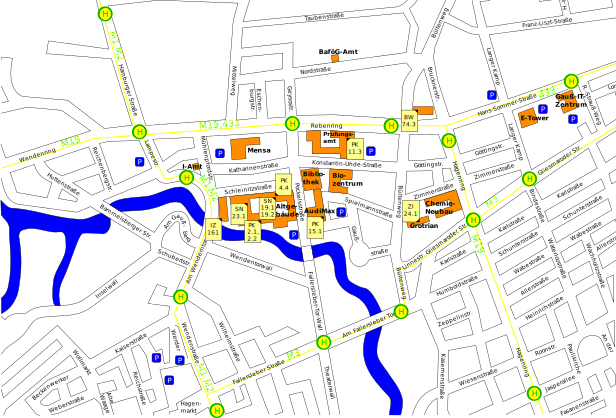
\includegraphics[angle=90, width=\textwidth]{bilder/plan.pdf}
%  \end{figure*}
%  \clearpage
%  \setcounter{page}{1}

%  
\section{Vorwort}
\label{vorwort}
	\begin{multicols}{2}
	\subsection*{Willkommen in der Informatik!}	

	Ein neues Semester hat begonnen und wieder strömen unzählige neue Gesichter auf den Campus um das Abenteuer Studium zu beginnen oder fortzusetzen. Da das nicht immer ganz einfach ist haben wir, die Fachgruppe Informatik für die Erstsemester unserer Fachrichtung einen kleinen Leitfaden zusammengestellt - die 1-te.

	Auf den folgenden Seiten werden wir hoffentlich einige der typischen Fragen beantworten, die einen am Anfang des Studiums quälen. Außerdem möchten wir natürlich uns, die Fachgruppe vorstellen (s. Seite \pageref{fachgruppe}) und eventuell noch die ein oder andere hilfreiche Information mitgeben. 

	\subsubsection*{Aufbau dieses Heftes}
		In der ersten Hälfte dieses Heftes sind wichtige
		Erklärungen zum Studienbeginn, dem Studiengang und der
		universitären Infrastruktur. Weitere Informationen zu
		uns und unserer Gremienarbeit, sowie weitere
		Informationen sind in der zweiten Hälfte.
\columnbreak
	\subsubsection*{Die Fachgruppe Online}
		Natürlich gibt es uns auch online - auf der Seite \url{http://fginfo.cs.tu-bs.de}. Beispielsweise stehen dort aktuelle Termine wie Spiele- oder Grillabende. Auch gibt es dort noch einmal die Inhalte dieses Heftes, samt den Aktualisierungen die erst nach dem Druck bekannt wurden. 

	\vspace*{0.5cm}

	Viel Spaß und Erfolg im  Studium wünscht  die\\
	\hspace*{2cm}Fachgruppe Informatik
	\end{multicols}
	\vspace{0.5cm}
	\begin{center} 
\includegraphics[totalheight=12cm]{bilder/XKCD/dorm_poster}
\end{center}

%\end{multicols}
\renewcommand{\baselinestretch}{0.85}\normalsize
  \newpage
%  \ntoc %% Inhaltsverzeichnis
  \clearpage
  \newpage

    \begin{multicols}{2}
%
\end{multicols}
\section*{Das Wichtigste für den Bachelor}
  Auf detailiertere Informationen in der vollständigen Ausgabe der 1-ten wird wie folgt
  verwiesen: \mehrInfo{Abschnitt, Seite}.%%
\end{multicols}
\subsection*{Termine}
In der Tabelle steht das B für Bachelor und das M für Master.
\mehrInfo{,,Die ersten Tage'', Seite 3 \& 4}.
\begin{tabular}{|l|l|p{6.7cm}|c|c|c|}
\hline \textbf{Datum} & \textbf{Uhrzeit} & \textbf{Veranstaltung}	& \textbf{Ort} & \textbf{B} & \textbf{M} \\
\hline 26.09. – 30.09.	& 1. Tag: 10:00	 & Vorkurs Informatik
& PK 2.1		&B& \\
17.10. - 21.10.  & & & & &    \\
%\hline 11.10. – 22.10. 	&		 & Vorkurs Mathematik 								&				&B& \\
\hline Montag,  24.10. 	&  09:00 – 10:00	 & Begrüßung	durch den Präsidenten									& Stadion		&B&M\\ % TODO wirklich Audimax?
\hline 			& 10:00 – 12:00	 & Infobörse										& Altgebäude	&B&M\\
\hline   	& 10:00 – 11:00	 & Begrüßung (M) \newline durch den Studiendekan	& IZ 160	& &M\\
\hline 	& 11:30 – 13:00	 & Ersti-Frühstück									& IZ Plaza		&B&M\\
\hline 			& 13:05 – 14:00	 & Einführung  der Fachgruppe					& IZ 160		&B&M\\
\hline 			& 14:00 – 15:00	 & Begrüßung (B) \newline
durch den Studiendekan	& PK 11.3	&B& \\
\hline 			& 15:00 – 16:30	 & Erste Vorlesung
,,Programmieren 1''				& SN 19.1		&B &\\
%\hline 			& 14:00 – 15:00	 & Gemeinsames Stundenplan-Bauen					& IZ 161		& &M\\
%\hline 			& 15:00 – 16:30	 & Rundgang mit der Tutorengruppe					& SN 19.1		&B&M \\
%
%
%\hline 			& 15:00 – 15:30	 & Rundgang  \newline mit der Tutorengruppe		& IZ 150		&B&M \\
%\hline 			& 15:30 – 16:30	 & Gemeinsames Stundenplan-Bauen					& IZ 161		& B&\\
\hline Dienstag, 25.10		& 10:00 - 11:45 &
Erstsemester-Frühstück & IZ Plaza & B &M \\ 
\hline & 12:00 - 13:30 * & FG-Einführung und  \newline
Stundenbahn-Bauen & ??? * & B &\\%& ??? * & B &\\
\hline & 12:00-13:30 * & FG-Einführung und   \newline Stundenbahn-Bauen & IZ 160 * & & M\\
\hline &13:30 - 15:00 & Rundgang mit den  Tutorengruppen & IZ 160 & B
& M\\
\hline Donnerstag, 03.11 & 19:00 & Kneipentour der Fachgruppe & IZ 150 & B & M\\
\hline Mittwoch, 09.11 & 19:00 & Spieleabend der Fachgruppe & vor  150 & B & M\\
%17:00 – \ldots & Grillen / Spieleabend  mit
%der Fachgruppe (wetterabhängig :) )
%& siehe Blog		&B&M\\
%\hline 27.10.	& 10:00 – 17:00	 & Studium Generale									& Altgebäude	&B&M\\
%\hline 15.04.	& 19:00 – \ldots & Kneipentour mit der Fachgruppe					& IZ 150		&B&M\\
%\hline 10.11.	& 16:30 – \ldots & Spieleabend der Fachgruppe						& vor IZ 150	&B&M\\ 
\hline
\end{tabular} 

%%% Local Variables: 
%%% mode: latex
%%% TeX-master: "../../1-te"
%%% End: 

\subsection*{Checkliste}
% !TEX root = ../../1-te.tex

\begin{center}
\begin{tabular}{|p{3mm}|l|p{8cm}|c|c|}
\hline \checkmark 
       & \textbf{Todo}             & \textbf{Zu erledigen bis}                                  & \textbf{Seite}               & \textbf{Muss?} \\ 
\hline & BAföG beantragen          & Spätestens Ende \iftoggle{winter}{Oktober}{April}          & \pageref{todobafoeg}         & optional \\ 
\hline & Wohnsitz ummelden         & 1 Woche nach Umzug                                         & \pageref{todoummelden}       & ja \\
\hline & Mailinglisten             & So früh wie möglich                                        & \pageref{mailinglisten}      & ja \\ 
\hline & Studiengrobplanung        & Vor dem Stundenplan bauen                                  & \pageref{grob}               & ja \\
\hline & Auflagen klären           & So früh wie möglich, final: Ende 2. Semester               & \pageref{auflagen}           & nur Master \\ 
\hline & Persönlicher Stundenplan  & Siehe Terminzettel der Fachgruppe                          & \pageref{masterstundenplan}  & ja \\ 
\hline & Prüfungsbogen             & Spätestens \iftoggle{winter}{Dezember}{Mai}                & \pageref{todoanmeldung}      & ja \\ 
\hline & Prüfungsanmeldung         & 12.12.2017 - 11.01.2018, schriftlich oder online           & \pageref{todoanmeldung}      & ja \\ 
\hline & Blog abonnieren           & So früh wie möglich                                        & \pageref{fachgruppe}         & ja \\ 
\hline & Prüfungsordnung lesen     & Zu den ersten Klausuren                                    & \pageref{po}                 & ja \\ 
\hline & TUcard validieren         & Zu Beginn und zu jedem neuen Semester                      & \pageref{tucard}             & ja \\
\hline & Bibliotheksausweis        & Vor der ersten Buchausleihe                                & \pageref{todobib}            & optional \\
\hline & Stud.IP-Nachrichten weiterleiten  & Wenn man nichts verpassen möchte         & \pageref{tumails}            & optional \\
\hline
\end{tabular} 
\end{center}
\tocheck{4}{Exakte Daten Anmeldewoche einfügen, s.\url{https://www.tu-braunschweig.de/fk1/service/informatik/pa}}
%
%
\begin{multicols}{2}
\subsection*{Tutorien}
Nach dem Erstsemesterfrühstück werden die Erstsemester nach Bachelor und
Master getrennt in Tutorengruppen aufgeteilt. Diese kleinen Gruppen erkunden den Campus. Auftretende Fragen sollten dem Tutor gestellt werden. Im 
\mehrInfo{Abschnitt Tutorien, Seite 5} findet ihr sowohl mehr Informationen, als auch Bilder und Emailadressen
einiger Tutoren.%\newpage
\subsection*{Studienplanung}
Pro Semester sollten ungefähr 30 Credits erreicht werden, damit man in
6 Semestern den Bachelor und in 4 den Master besteht.
Der folgende Stundenplan für das 1. Semester und der Studienplan ist lediglich ein Vorschlag an den ihr nicht gebunden seid. Weitere Informationen:\\
\mehrInfo{Allgemeine Studienplanung ab  Seite 7}\\
\mehrInfo{ Zum Bachelor ab Seite
  18 }\\
\subsection*{Ansprechpartner}
Zunächst einmal wäre da für Vorlesungen der jeweilige Dozent zu nennen,
keiner beißt :) Auerdem könnt ihr uns als Fachgruppe unter
\nurl{fginfo@tu-bs.de}  erreichen. Außerdem treffen wir uns regelmäßig,
die Termine findet ihr unter
\nurl{http://fginfo.cs.tu-bs.de/index.php/fachgruppe/fachgruppenrat/}
Es gibt aber noch eine Menge anderer Ansprechpartner
(Studiengangskoordinatorin, Studienberatung etc):
\mehrInfo{Abschnitt Sonstiges, Seite 54}. 

\subsection*{Wichtige Links}
\begin{description}
  \item[TU-Homepage]~\\\nurl{http://tu-braunschweig.de/}
 \item[Hauptseite der Informatik]~\\\nurl{http://www.cs.tu-bs.de/}
 \item[Fachgruppenrat Informatik]~\\\nurl{http://fginfo.cs.tu-bs.de/}
 \item[Fachbereichssekretariat / Prüfungsamt]~\\
 \nurl{http://tu-braunschweig.de/fk1/service/informatik}\\
\item[Gesamtstundenplan]~\\\nurl{http://www.cs.tu-bs.de/stundenplan/}\\
\item[Vorlesungsverzeichnis]~\\\nurl{http://vorlesungen.tu-bs.de/}\\
\item[Inoffielles Forum von Studis für
  Studis]~\\\nurl{https://www.clevershit.de/}\\
\item[Modulhandbuch]~\\\nurl{http://mhb.tu-bs.de/}\\
%\item[Allgemeines Vorlesungsverzeichnis:] ~\\
%{\footnotesize\url{http://vorlesungen.tu-bs.de}}
\item[Uni-Bibliothek:] ~\\\nurl{http://www.biblio.tu-bs.de}
\item[Druckkosten:] ~\\\nurl{http://www.tu-braunschweig.de/it/services/drucken/kosten}
\item[Don't panic online] ~\\
{\footnotesize\url{http://www.tu-braunschweig.de/Medien-DB/it/dontpanic.pdf}}
\end{description}

\subsection*{Sonstiges}
Hier findet ihr Verweise zu mehr oder wichtigen Themen, auf die wir hier
aber aus Platzgründen nicht näher eingehen können:
\begin{description}
  %\item[27C3]~Das große Hackertreffen und du bist dabei\\\mehrInfo{Seite 55}
\item[Computer]~in der Informatik oder etwa nicht?\\\mehrInfo{Seite 34}
  \item[Freizeit] Es gibt ein Leben neben dem Studium\\\mehrInfo{Seite
    44} 
% TODO
%  \item[Interview] Ein Dozent erzählt \mehrInfo{}
\item[Gruppen und Unipolitik]~Bildungspolitik für alle\\\mehrInfo{Seite
  48}
\item[Lernräume] Asyl für den Prüfungszeitraum\\\mehrInfo{Seite 55}
  \item[Semesterticket] Spaß mit der Deutschen Bahn\\\mehrInfo{Seite 56}
\end{description}

\end{multicols}
\includegraphics[totalheight=0.4\textheight, 
width=\textwidth
]{texte/nuetzliches/stundenplan}
\includegraphics[angle=90,
totalheight=\textheight
, width=\textwidth]{texte/bachelor/studienplan_neu}
\newpage
\begin{multicols}{2}


%\end{figure}
 %     \subsection{Tutorien}
Da der Einstieg ins Studium alleine relativ schwierig ist und sich viele Fragen in einer Gruppe am einfachsten beantworten lassen, gibt es Tutorengruppen, denen du am Montag um ca. 15 Uhr zugeteilt wirst. 
In diesen findet dann ein Rundgang über den Campus und die wichtigsten Einrichtungen in der Nähe statt. 
Dort hast du außerdem die Möglichkeit in überschaubarer Runde andere Informatikstudenten und eben eure Tutoren kennen zu lernen, sowie weitere Informationen zu deinen Veranstaltungen und Dozenten zu erhalten.
Scheu dich nicht, einen der Tutoren zu kontaktieren. Da weitere Treffen geplant sind kannst du dich auch nachträglich noch in eine Tutorengruppe einteilen lassen. Dazu schreibt bitte eine Mail an die Fachgruppe \url{fginfo@tu-bs.de} oder direkt an einen der Tutoren.


\ifpdf
Damit du schonmal das ein oder andere Gesicht kennst, sind hier die Fotos der Tutoren abgebildet.
%%
\end{multicols}



% TODO Bilder aktualisieren, angeben, ob der jenige Bachelors oder Masters betreut (ist ja nicht immer identisch damit, was man selbst gerade ist)
% NICHT als \paragraph, da das leider das Layout verhaut. Ist natürlich
% unschön ):
%Leider ist das ganze Layout etwas screwed
%Also ein alter Trick aus Web 1.0 Tagen\ldot.
%Layout Tabellen! Nicht schön, aber wenns sonst nicht geht\ldot.
  \begin{tabular}{c}
\begin{tabular}{lll}
  { \textbf{Bachelor Tutoren}} \ \\ 
% \picture[0.3\linewidth]
% {bilder/tutoren/kris.jpg}
% {Christoph\\ 3. Semester Master\\ \randomize{admin@keeg.de}}
% \ {
{
\picture[0.3\linewidth]
{bilder/tutoren/dominik_pass}
{Dominik\\%3. Semester Master\\ 
\randomize{d.schuermann@tu-bs.de}}
}%\hfill
& \ 
%{\picture[2.3\linewidth]
%{bilder/tutoren/franziska.jpg}
%{Franziska\\6. Semester Bachelor\\ \randomize{f.werk@tu-bs.de}}
%}%\\ \ \\
{\picture[0.3\linewidth]
{bilder/tutoren/jan_germann.jpg}
{Jan\\%2. Semester Bachelor\\ 
\randomize{j.germann@tu-bs.de}}
} 
&\
{
\picture[0.3\linewidth]
{bilder/tutoren/hf}
{Hella\\% 2. Semester Master\\ 
\randomize{h-f.hoffmann@tu-bs.de}}}
\\ \  \\
%\hfill
{\picture[0.3\linewidth]
{bilder/tutoren/johannes.jpg}
{Johannes\\% 7. Semester Bachelor\\ 
\randomize{J.Starosta@tu-bs.de}}
}& \ 
%\hfill
% {\picture[0.3\linewidth]
% {bilder/tutoren/judith.jpg}
% {Judith\\ 5. Semester Bachelor\\ \randomize{judith.hilpert@web.de}}}\\
% \ \\
% \picture[0.3\linewidth]
% {bilder/tutoren/marekd.jpg}
% {Marek\\ 1. Semester Master\\ \randomize{m.drogon@tu-bs.de}}
% &  %\hfill
 {
 \picture[0.3\linewidth]
 {bilder/tutoren/sebastian.jpeg}
 {Sebastian\\ %9. Semester Bachelor\\ 
\randomize{se.busse@tu-bs.de}}} 
%&{
%\picture[0.3\linewidth]%{}
%{bilder/tutoren/serj}
%{Serj\\ 1. Semester Master\\\randomize{s.dechand@tu-bs.de }}}
%\par \ \par  
%\end{tabular}
%
%\begin{center}
%  \begin{tabular}{ccc}
 %    { \picture[0.3\linewidth]%{}
 % {bilder/tutoren/christina}
 % {Christina\\ 5. Semester Bachelor\\\randomize{c.eberth@tu-bs.de}}}
%{
%\picture[0.3\linewidth]%{}
%{bilder/tutoren/viktor}
%{Viktor Richert\\ 4. Semester Bachelor\\%}%\\ 5. Semester Bachelor\\
%\randomize{InformatikWiki@gmx.de}}%.eberth@tu-bs.de }
% }&{
%  \picture[0.3\linewidth]%{}
%  {bilder/tutoren/dummy}
%  {Christoph\\ 5. Semester Bachelor\\ \randomize{christoph.harburg@web.de}}
% }\\
&\ {\picture[0.3\linewidth]%{}
{bilder/tutoren/joko_n}
{Jonathan\\% 7. Semester Bachelor \\
\randomize{j.koscielny@tu-bs.de}}}
\\ \  \\
{\picture[0.3\linewidth]%{}
{bilder/tutoren/viktor}
{Viktor\\% 5. Semester Bachelor\\%\\ 5. Semester Bachelor\\
\randomize{InformatikWiki@gmx.de}}}
&\ {\picture[0.3\linewidth]%{}
{bilder/tutoren/rcfinster_sm}
{Rebecca \\ % Bachelor\\%}%\\ 5. Semester Bachelor\\
\randomize{r.finster@tu-bs.de}}}
& \ 
{\picture[0.3\linewidth]
{bilder/tutoren/keno_sw.jpg}
{Keno\\%2. Semester Bachelor\\ 
\randomize{k.garlichs@tu-bs.de}}
}
\end{tabular}%\tabularnewline \\
\end{tabular}\tabularnewline \\
%\begin{left}
\newpage
%\begin{center}
\begin{tabular}{ccc}
{ \textbf{Master Tutoren}}\\
% NICHT als \paragraph, da das leider das Layout verhaut. Ist natürlich
% unschön ):
\picture[0.3\linewidth]
{bilder/tutoren/martinw_sw.jpg}
{Martin\\% 4. Semester Master\\ 
\randomize{m.wegner@tu-bs.de}}
&
%{ 
%\picture[0.3\linewidth]
%{bilder/tutoren/jan.jpg}
%{Till\\  Master\\ \randomize{t.lorentzen@tu-bs.de}
%}&
%\\
%\hfill %\par \ \par
%{
%\picture[0.3\linewidth]
%{bilder/tutoren/henning.jpg}
%{Henning\\ 5. Semester Master\\ \randomize{h.guenther@tu-bs.de}}
%}&
{ 
\picture[0.3\linewidth]
{bilder/tutoren/sophia.jpg}
{Sophia\\% 3. Semester Master\\
\randomize{s.scholtka@tu-braunschweig.de}}
}
&
{
\picture[0.3\linewidth]%{}
{bilder/tutoren/serj}
{Serj\\% 2. Semester Master\\
\randomize{s.dechand@tu-bs.de }}}
\\ \ \\
{\picture[0.3\linewidth]
{bilder/tutoren/lena_sm.jpg}
{Lena\\ %5. Semester Master\\ 
\randomize{dielenamaria@gmail.com}}
}&
%\hfill
%{\picture[0.3\linewidth]
%{bilder/tutoren/hashier.jpg}%Christopher Lössl < c.loessl@tu-bs.de>
%{Chris \\3. Semester Master\\ \randomize{c.loessl@tu-bs.de}}
%}%&
{\picture[0.3\linewidth]
{bilder/tutoren/till_sw}
{Till\\ %\\  4. Semester Master\\
\randomize{t.lorentzen@tu-bs.de}}
}
%\picture[0.3\linewidth]
%{bilder/tutoren/stephan.jpg}
%{Stephan\\ 5. Semester Master\\ stephan.friedrichs@tu-bs.de}
  \end{tabular}
%  \end{tabular}
  
%\end{center}
\else
In der Druckfassung wären hier die Tutoren mit Emailadresse und Foto aufgelistet. Um die Privatspäre der Tutoren zu schützen, stehen diese jedoch nicht direkt hier in der Onlinefassung.
\fi

%%
%
\begin{multicols}{2}
% Local Variables: 
% mode: latex
% TeX-master: "../../1-te"
% End: 

%  %%
\end{multicols}
%\section{Errata}
%Seit dem Druck der 1-ten wurde folgendes berichtigt:
%\begin{itemize}
%\item Der Link zu den WLAN-Infos war tot
%\item Im herausnehmbaren Inlay waren noch alte Studienpläne drin (im eigentlichen Heft war's schon korrekt)
%\end{itemize}
\section{Die ersten Tage}
%%
%
\begin{multicols}{2}
\subsection{Termine}
\label{termine}
	\begin{multicols}{2}
	Gerade in der Anfangszeit des Studiums gibt es eine Menge zu tun. Damit du
	nicht das Wichtigste verpasst, haben wir die ersten Termine kompakt für
	dich zusammengefasst. Die meisten davon bieten die Gelegenheit Fragen zu
	stellen und nebenbei gleich ein paar nette Kommilitonen kennen zu lernen.

	Falls du  es dir nicht schon gedacht habt: Die Spalten B und M geben an,
	ob der Termin für Bachelor- oder Masterstudenten gedacht
        ist. Falls du den eigentlichen Termin verpasst, kannst du
        stattdessen auch zum anderen erscheinen. Es besteht die Chance, dass sich einige Orte
	und Zeiten
	nach Drucklegung noch Ändern.  Bei den mit ,,*'' markierten Zeiten und
	Orten ist das besonders wahrscheinlich. Schaue deshalb bitte vorher
	nochmal im Blog \url{http://fginfo.cs.tu-bs.de/} nach, ob die Angaben
	noch aktuell sind. Dort kannst du übrigens auch den Kalender digital abonnieren.
	Du findset die Termine auch online unter \url{http://tinyurl.com/3ltuzbb}.
	Wenn du einen Dienst, ein Handy oder eine Software nutzt, die das iCalender-Format unterstützt
	kannst du die Termine auch von dort aus einbinden und hast sie somit im Blick. 
	Dazu gehören z.\,B. iPhone, Android, Google Calendar, Outlook\,\dots. Eine Liste 
	von ca. 60 Programmen findest du unter 	\url{http://tinyurl.com/yns84t}
	\end{multicols}

	\begin{tabular}{|l|l|p{6.7cm}|c|c|c|}
	\hline \textbf{Datum} 		& \textbf{Uhrzeit} 	& \textbf{Veranstaltung}						& \textbf{Ort} 	& \textbf{B}	& \textbf{M} 	\\
	\hline 26.09. – 30.09.		& 1. Tag: 10:00	 	& Vorkurs Informatik							& PK 2.1		& B				& 				\\
		   17.10. – 21.10.		& 					& 												& 				& 				&    			\\
	\hline Mo, 24.10. 			& 09:00 – 10:00		& Begrüßung	durch den Präsidenten				& Stadion		& B				& M				\\ 
	\hline 						& 10:00 – 12:00	 	& Infobörse										& Altgebäude	& B				& M				\\
	\hline   					& 10:00 – 11:00	 	& Begrüßung (M) \newline durch den Studiendekan	& IZ 160		& 				& M				\\
	\hline 						& 14:00 – 15:00	 	& Begrüßung (B) \newline durch den Studiendekan	& PK 11.3		& B				& 				\\
	\hline 						& 15:00 – 16:30		& Erste Vorlesung ,,Programmieren 1''			& SN 19.1		& B 			&				\\
	\hline Di, 25.10.			& 10:00 – 11:45 	& Erstsemester-Frühstück 						& IZ Plaza 		& B 			& M 			\\ 
	\hline 						& 12:00 – 13:30 * 	& FG-Einführung und \newline Stundenplan-Bauen 	& ??? * 		& B 			&  				\\%& ??? * & B &\\
	\hline 						& 12:00 – 13:30 * 	& FG-Einführung und \newline Stundenplan-Bauen 	& IZ 160 * 		& 				& M				\\
	\hline 						& 13:30 – 15:00 	& Rundgang mit den  Tutorengruppen 				& IZ 160 		& B 			& M				\\
	\hline Mi, 26.10.			& 10:00 – 17:00		& Studium Generale								& Altgebäude	& B				& M 			\\
	\hline Do, 03.11. 			& 19:00 			& Kneipentour der Fachgruppe 					& IZ 150 		& B 			& M				\\
	\hline Mi, 09.11.	 		& 19:00 			& Spieleabend der Fachgruppe 					& vor  150 		& B 			& M				\\
	\hline
	\end{tabular} 
%
%	\begin{multicols}{2}
%	Ihr findet die Termine auch online unter \url{http://tinyurl.com/3ltuzbb}.
%	Falls ihr einen Dienst, ein Handy oder eine Software nutzt, die das iCalender-Format unterstützt
%	könnt ihr die Termine auch von dort aus einbinden und habt sie somit im Blick. 
%	Dazu gehören z.\,B. iPhone, Android, Google Calendar, Outlook\,\dots. Eine Liste 
%	von ca. 60 Programmen findet ihr unter 
%	\url{http://tinyurl.com/yns84t}
%	\end{multicols}

% !TEX root = ../../1-te.tex

\subsection{Checkliste}
\label{checkliste}
	Hier wird zusammengefasst, was du in den ersten Tagen des Studiums unbedingt erledigen solltest. Wenn du die ToDos auf der Checkliste nach Erledigung abhakst, verlierst du nicht den Überblick und vergisst nichts.
	
\vspace*{0.5cm}
\input{texte/erstetage/tabcheck}

\begin{multicols}{2}

\subsubsection{BAföG}
	\label{todobafoeg}

	Wer Studierendenförderung nach dem Bundesausbildungsförderungsgesetz (BAföG) beantragen möchte, sollte sich am besten gründlich informieren. Sehr zu empfehlen ist da: \\
	\verUrl{4}{https://www.xn--bafg-7qa.de/}
 
	Förderungsanträge gibt es zum Download oder in Papierform im EG des Amtes für Ausbildungsförderung in der Wilhelmstraße 1. Wenn du BAföG beantragen möchtest, stelle den Antrag so früh wie möglich, denn es wird nicht rückwirkend gezahlt.

	Zum Anfang des Semester ist mit längeren Wartezeiten zu rechnen, im Notfall kannst du beim AStA-Sozialreferat ein kurzfristiges, zinsloses Darlehen beantragen, um den ersten Monat zu überbrücken. Das Darlehen ist auf 450 Euro begrenzt und muss spätestens nach drei Monaten zurückgezahlt werden. Mehr Informationen findest du auf der Seite des Sozialreferats: \verUrl{4}{https://www.asta.tu-braunschweig.de/referate/sozialreferat/}


\subsubsection{Ummelden}
	\label{todoummelden}

	Wer neu nach Braunschweig gezogen ist, muss sich innerhalb einer Woche beim Einwohnermeldeamt anmelden. Wenn ihr die Frist verpasst, drohen theoretisch Strafen, aber praktisch sieht es da nicht so streng aus. Wenn man Braunschweig als Erstwohnsitz wählt, bekommt man (ein Jahr später) eine einmalige Zuzugsprämie von 100 Euro (Immatrikulationsbescheinigung nicht vergessen). Alternativ kann man Braunschweig auch als Zweitwohnsitz wählen.

\subsubsection{Prüfungsanmeldung}
	\label{todoanmeldung}

	Du musst dich für alle Prüfungen, an denen du teilnehmen willst, vorher beim Prüfungsamt anmelden. Die Fristen sind relativ früh im Semester. Die Termine werden im Laufe des Semesters veröffentlicht (Seiten des P-Amtes (\verUrl{3}{https://www.tu-braunschweig.de/fk1/service/informatik/pa}), Mailingliste). Prüfungen können im Prüfungsanmeldezeitraum schriftlich im Prüfungsamt oder online über das QIS-Portal angemeldet werden.
	Vor deiner ersten Prüfungsanmeldung musst du außerdem ein Datenblatt ausfüllen. Es empfiehlt sich, das bereits vor der Anmeldewoche zu machen, weil die Schlangen dann nicht so lang sind.

	Für die Online-Anmeldung benötigst du eine TAN-Liste, die du dir vorher im Prüfungsamt organisieren musst.

	Unter folgendem Link findest du außerdem alle Prüfungstermine für die Informatik:
	\verUrl{3}{https://www.tu-braunschweig.de/fk1/service/informatik/pa}

\subsubsection{TUcard}
	\label{tucard}
	
	Alle Studierenden der TU erhaten den elektronische Studierendenausweis TUcard, die auch als Bibliotheksausweis und Mensakarte genutzt werden kann.

	Damit die Karte gültig ist, muss sie zu Beginn und zu jedem neuen Semester validiert werden. Das bedeutet, dass der Thermostreifen auf der Karte in einem Validierungsdrucker mit den aktuellen Daten beschrieben wird.

	Das Börsenguthaben der Karte, beispielsweise zum Bezahlen in der Mensa, kann an Börsenaufwertern (auch denen, die sich bereits in den Mensen befinden) aufgeladen werden.

	Zum Drucken kann Guthaben der Karte auf ein Druckkonto umgebucht werden. Dies geschieht an den Druckkontenumbuchern.

	Weitere Informationen zur TUcard findest du unter: \verUrl{3}{https://www.tu-braunschweig.de/studium/imstudium/tucard}

\subsubsection{Uni-Bibliothek}
	\label{todobib}

	Um Bücher in der Uni-Bibliothek ausleihen zu können, brauchst du einen Ausweis. Dieser ist in deiner TUcard integriert. Diesen kannst du an einem der Terminals in der Bibliothek, oder online beantragen und am Schalter freischalten. Je nachdem, ob du zu Beginn schon Bücher brauchst, kannst du die Karte auch später aktivieren.

	In der Bibliothek stehen außerdem Kopierer bereit, die du nutzen kannst. Einen davon kannst du mit Kleingeld befüllen, kompfortabler geht es aber mit einer Kopierkarte. Die bekommst du für ein paar Euro direkt in der Bibliothek. Zu Semesterbeginn gibt es oft noch Einführungskurse in die Bibliotheksbenutzung. Ob du deinen Bibliotheksausweis vor oder nach diesem Kurs aktivierst, ist egal.
	
\end{multicols}

\subsection{Tutorien}
Da der Einstieg ins Studium alleine relativ schwierig ist und sich viele Fragen in einer Gruppe am einfachsten beantworten lassen, gibt es Tutorengruppen, denen du am Montag um ca. 15 Uhr zugeteilt wirst. 
In diesen findet dann ein Rundgang über den Campus und die wichtigsten Einrichtungen in der Nähe statt. 
Dort hast du außerdem die Möglichkeit in überschaubarer Runde andere Informatikstudenten und eben eure Tutoren kennen zu lernen, sowie weitere Informationen zu deinen Veranstaltungen und Dozenten zu erhalten.
Scheu dich nicht, einen der Tutoren zu kontaktieren. Da weitere Treffen geplant sind kannst du dich auch nachträglich noch in eine Tutorengruppe einteilen lassen. Dazu schreibt bitte eine Mail an die Fachgruppe \url{fginfo@tu-bs.de} oder direkt an einen der Tutoren.


\ifpdf
Damit du schonmal das ein oder andere Gesicht kennst, sind hier die Fotos der Tutoren abgebildet.
%%
\end{multicols}



% TODO Bilder aktualisieren, angeben, ob der jenige Bachelors oder Masters betreut (ist ja nicht immer identisch damit, was man selbst gerade ist)
% NICHT als \paragraph, da das leider das Layout verhaut. Ist natürlich
% unschön ):
%Leider ist das ganze Layout etwas screwed
%Also ein alter Trick aus Web 1.0 Tagen\ldot.
%Layout Tabellen! Nicht schön, aber wenns sonst nicht geht\ldot.
  \begin{tabular}{c}
\begin{tabular}{lll}
  { \textbf{Bachelor Tutoren}} \ \\ 
% \picture[0.3\linewidth]
% {bilder/tutoren/kris.jpg}
% {Christoph\\ 3. Semester Master\\ \randomize{admin@keeg.de}}
% \ {
{
\picture[0.3\linewidth]
{bilder/tutoren/dominik_pass}
{Dominik\\%3. Semester Master\\ 
\randomize{d.schuermann@tu-bs.de}}
}%\hfill
& \ 
%{\picture[2.3\linewidth]
%{bilder/tutoren/franziska.jpg}
%{Franziska\\6. Semester Bachelor\\ \randomize{f.werk@tu-bs.de}}
%}%\\ \ \\
{\picture[0.3\linewidth]
{bilder/tutoren/jan_germann.jpg}
{Jan\\%2. Semester Bachelor\\ 
\randomize{j.germann@tu-bs.de}}
} 
&\
{
\picture[0.3\linewidth]
{bilder/tutoren/hf}
{Hella\\% 2. Semester Master\\ 
\randomize{h-f.hoffmann@tu-bs.de}}}
\\ \  \\
%\hfill
{\picture[0.3\linewidth]
{bilder/tutoren/johannes.jpg}
{Johannes\\% 7. Semester Bachelor\\ 
\randomize{J.Starosta@tu-bs.de}}
}& \ 
%\hfill
% {\picture[0.3\linewidth]
% {bilder/tutoren/judith.jpg}
% {Judith\\ 5. Semester Bachelor\\ \randomize{judith.hilpert@web.de}}}\\
% \ \\
% \picture[0.3\linewidth]
% {bilder/tutoren/marekd.jpg}
% {Marek\\ 1. Semester Master\\ \randomize{m.drogon@tu-bs.de}}
% &  %\hfill
 {
 \picture[0.3\linewidth]
 {bilder/tutoren/sebastian.jpeg}
 {Sebastian\\ %9. Semester Bachelor\\ 
\randomize{se.busse@tu-bs.de}}} 
%&{
%\picture[0.3\linewidth]%{}
%{bilder/tutoren/serj}
%{Serj\\ 1. Semester Master\\\randomize{s.dechand@tu-bs.de }}}
%\par \ \par  
%\end{tabular}
%
%\begin{center}
%  \begin{tabular}{ccc}
 %    { \picture[0.3\linewidth]%{}
 % {bilder/tutoren/christina}
 % {Christina\\ 5. Semester Bachelor\\\randomize{c.eberth@tu-bs.de}}}
%{
%\picture[0.3\linewidth]%{}
%{bilder/tutoren/viktor}
%{Viktor Richert\\ 4. Semester Bachelor\\%}%\\ 5. Semester Bachelor\\
%\randomize{InformatikWiki@gmx.de}}%.eberth@tu-bs.de }
% }&{
%  \picture[0.3\linewidth]%{}
%  {bilder/tutoren/dummy}
%  {Christoph\\ 5. Semester Bachelor\\ \randomize{christoph.harburg@web.de}}
% }\\
&\ {\picture[0.3\linewidth]%{}
{bilder/tutoren/joko_n}
{Jonathan\\% 7. Semester Bachelor \\
\randomize{j.koscielny@tu-bs.de}}}
\\ \  \\
{\picture[0.3\linewidth]%{}
{bilder/tutoren/viktor}
{Viktor\\% 5. Semester Bachelor\\%\\ 5. Semester Bachelor\\
\randomize{InformatikWiki@gmx.de}}}
&\ {\picture[0.3\linewidth]%{}
{bilder/tutoren/rcfinster_sm}
{Rebecca \\ % Bachelor\\%}%\\ 5. Semester Bachelor\\
\randomize{r.finster@tu-bs.de}}}
& \ 
{\picture[0.3\linewidth]
{bilder/tutoren/keno_sw.jpg}
{Keno\\%2. Semester Bachelor\\ 
\randomize{k.garlichs@tu-bs.de}}
}
\end{tabular}%\tabularnewline \\
\end{tabular}\tabularnewline \\
%\begin{left}
\newpage
%\begin{center}
\begin{tabular}{ccc}
{ \textbf{Master Tutoren}}\\
% NICHT als \paragraph, da das leider das Layout verhaut. Ist natürlich
% unschön ):
\picture[0.3\linewidth]
{bilder/tutoren/martinw_sw.jpg}
{Martin\\% 4. Semester Master\\ 
\randomize{m.wegner@tu-bs.de}}
&
%{ 
%\picture[0.3\linewidth]
%{bilder/tutoren/jan.jpg}
%{Till\\  Master\\ \randomize{t.lorentzen@tu-bs.de}
%}&
%\\
%\hfill %\par \ \par
%{
%\picture[0.3\linewidth]
%{bilder/tutoren/henning.jpg}
%{Henning\\ 5. Semester Master\\ \randomize{h.guenther@tu-bs.de}}
%}&
{ 
\picture[0.3\linewidth]
{bilder/tutoren/sophia.jpg}
{Sophia\\% 3. Semester Master\\
\randomize{s.scholtka@tu-braunschweig.de}}
}
&
{
\picture[0.3\linewidth]%{}
{bilder/tutoren/serj}
{Serj\\% 2. Semester Master\\
\randomize{s.dechand@tu-bs.de }}}
\\ \ \\
{\picture[0.3\linewidth]
{bilder/tutoren/lena_sm.jpg}
{Lena\\ %5. Semester Master\\ 
\randomize{dielenamaria@gmail.com}}
}&
%\hfill
%{\picture[0.3\linewidth]
%{bilder/tutoren/hashier.jpg}%Christopher Lössl < c.loessl@tu-bs.de>
%{Chris \\3. Semester Master\\ \randomize{c.loessl@tu-bs.de}}
%}%&
{\picture[0.3\linewidth]
{bilder/tutoren/till_sw}
{Till\\ %\\  4. Semester Master\\
\randomize{t.lorentzen@tu-bs.de}}
}
%\picture[0.3\linewidth]
%{bilder/tutoren/stephan.jpg}
%{Stephan\\ 5. Semester Master\\ stephan.friedrichs@tu-bs.de}
  \end{tabular}
%  \end{tabular}
  
%\end{center}
\else
In der Druckfassung wären hier die Tutoren mit Emailadresse und Foto aufgelistet. Um die Privatspäre der Tutoren zu schützen, stehen diese jedoch nicht direkt hier in der Onlinefassung.
\fi

%%
%
\begin{multicols}{2}
% Local Variables: 
% mode: latex
% TeX-master: "../../1-te"
% End: 


%  %
\end{multicols}
%\newpage
\section{Studienplan(ung) für jeden}
%\label{studienplan}
%
%
\begin{multicols}{2}
\subsection{Verantwortung}
	\textit{Große Macht bringt große Verantwortung mit sich!}, sagte schon Ben Parker, der Onkel von Spiderman. Das heißt für dich: Du hast die Macht und die Verantwortung über deinen Studienfortgang. Das beginnt bei der Entscheidung, überhaupt zu studieren, die Wahl des Faches und der Universität und erstreckt sich über die Wahl, welche Fächer du hörst und wann du das tust, bis hin zur Einflussnahme auf den gesamten Studiengang.

	Es besteht aber auch die Möglichkeit diese Verantwortung abzugeben. Es gibt einen Studienplan, der dir vorschlägt, wie du deine Fächer wählen und anordnen kannst, um in Regelstudienzeit fertig zu werden. Für den Bachelor sieht dieser Plan sehr konkret aus, für den Master ist er abstrakter gehalten, aber deckt immer noch nur partiell die Wahlmöglichkeiten ab. Das kann und soll er auch nicht -- es handelt sich um zwei von unendlich vielen Möglichkeiten, zum Studienabschluss zu kommen.	% Verantwortung
\subsection{Zwei Studiengänge unter einem Hut}
	Seit der Bologna-Reform gibt es an der TU Braunschweig zwei Studiengänge - \textit{Bachelor und Master}. Viele Informationen über das Studium betreffen beide, deshalb ist diese Zeitung für alle Erstsemester. Nach der allgemeinen Einleitung folgen die speziellen Abschnitte für Bachelor- (ab S. \pageref{bachelor}) und Master-Ersties (ab Seite \pageref{master}).

\subsubsection{Herden, Rudel und Einzelgänger}
	Bevor es in die Untiefen der Prüfungsordnungen und formalen Anforderungen geht, ein paar Worte zu einem sozialen Phänomen. Der recht feste Stundenplan im Bachelor-Studium sorgt dafür, dass man dort in der Regel mit vielen Mitstudierenden zusammensitzt, die in der gleichen Situation sind wie man selbst: Neu hier und mit den gleichen Fragen und Sorgen. Und ist ein Block zu Ende, so zieht man gemeinsam zum nächsten Raum, wo man mit praktisch der gleichen Gruppe das nächste Fach abgrast. Eine typische Herde also.

	Im Master ist das grundlegend anders. Jeder hört andere Vorlesungen, und in den \emph{Mastervorlesungen} tummeln sich nicht nur Masterstudierende, sondern auch Bachelor- und Diplom- oder gar fachverwandte Studierende, wie z.B. Wirtschaftsinformatik. Da kann es eine ganze Weile dauern, bis man weiß, wer auch im Masterstudium ist und gegebenfalls auch noch im gleichen Jahrgang. Selbst dann haben diese Leute ihren Bachelor hier oder dort, in diesem oder jenem Fach an einer Uni oder FH gemacht. Vielleicht haben die neben dir zuvor ganz andere Dinge gelernt, vielleicht sind sie hier um sich auf etwas komplett anderes zu spezialisieren als du.

	Keine Frage: Diese Mischung macht es spannender, bunter und vielseitiger, aber auf jeden Fall auch schwieriger. Wir können hier kaum Tipps geben, wie man als Neuling und eventuell unfreiwillige/r Einzelgänger/in ein kleines Rudel findet oder bildet. Weder wir noch dieses Heft könnten all das ersetzen, was eine Gruppe von Gleichgesinnten mit gleichen Problemen und Interessen könnte. Aber wir wissen, dass man in den ersten Tagen und Wochen viele Fragen hat. Gerade als Master hat man oft nur wenige Mitstudierende an der Seite, die die gleichen Fragen und/oder die passenden Antworten haben. Deshalb dieses Heft.

	Um deine Mitstudierenden schneller kennenzulernen, gibt es unter anderem die vielfältigen Angebote der Fachgruppe (Spieleabende, Kneipentouren, Grillen, etc.) - siehe \url{http://fginfo.cs.tu-bs.de/}
	% Bachelor und Master (Herden und Rudel)
\subsection{Die Prüfungsordnung}
\label{po}
	An einer Universität gibt es tausende Regeln und Ordnungen. Die wichtigste ist die Prüfungsordnung: Sie enthält Antworten auf 95\% aller Fragen, die im Studium auftreten - nicht nur wenn es um die eigentlichen Prüfungen geht. Die genaue Bezeichnung lautet \emph{Besonderer Teil der Prüfungsordnung für den (Bachelor-/Master-)studiengang Informatik der Technischen Universität Braunschweig}. Und da sie weder besonders lang, noch kompliziert geschrieben ist, sollte jeder Student sie einmal überfliegen.

	Außerdem gibt es noch die APO, die Allgemeine Prüfungsordnung. Sie gilt uniweit für alle Studiengänge, doch die beiden BPOs überschreiben die meisten APO-Regelungen.

	Wenn du es noch nicht getan hast, lade dir deine aktuelle Prüfungsordnung am besten von \url{http://www.tu-braunschweig.de/fk1/service/informatik/dokumente} herunter. 


		% Prüfungsordnung
% !TEX root = ../../1-te.tex

\subsection{Module und Co.}
	Um deinen Abschluss zu bekommen, musst du eine vordefinierte Menge von Modulen abdecken. Ein Modul besteht aus verschiedenen Bestandteilen.

\subsubsection{Vorlesung, Übung, etc.}
	\paragraph*{Vorlesung}
	Vorlesungen werden vor allen Studis abgehalten und befassen sich in erster Linie mit der theoretischen Herleitung des Stoffes. Solltest du in der Vorlesung einmal etwas nicht verstehen, so ist das nicht so tragisch. Vorlesungen an der Uni unterscheiden sich stark vom Unterricht an der Schule. Gehe nicht davon aus, Vorlesungsinhalte direkt zu verstehen. Plane eine gewisse Nachbearbeitungszeit für die Vorlesungen ein. In einer Vorlesung ist wegen der großen Teilnehmerzahl normalerweise kein Dialog mit dem oder der Vortragenden möglich. Aufgetretene Fragen können und sollten am besten direkt nach der Vorlesung oder sonst in einer Sprechstunde mit der oder dem Lehrenden geklärt werden.
	
	\paragraph*{Große Übung}
	Ergänzend gibt es die großen Übungen, auch Saalübungen genannt. Diese finden, wie die Vorlesung, vor dem gesamten Auditorium statt und sollen das erworbene, theoretische Wissen vertiefen und vor allem auch praktische, klausurbezogene Anwendungen aufzeigen. Die große Übung wird normalerweise von einer Mitarbeiterin oder einem Mitarbeiter gehalten. Sie sind bei  fachlichen Fragen kompetente Ansprechpartner/innen und meistens auch sehr hilfsbereit. Da sie  üblicherweise die Klausuren entwerfen, kann man bei genauem Hinhören in den großen Übungen oder im privaten Gespräch mit ihnen einiges über die Prüfung erfahren.

	\paragraph*{Kleine Übung, Seminargruppe}
	Als erstes eine Warnung: Kleine Übungen tauchen im Stundenplan nicht immer auf und werden leider nur in einigen Fächern angeboten. Der Begriff Seminargruppe ist synonym zu verstehen.
	
	In kleinen Übungen soll man selbst Aufgaben lösen. Dies geschieht unter Anleitung der HiWis (Hilfswissenschaftler/innen), welche meist Studierende höheren Semesters sind. Für die kleinen Übungen werden die Studis in etwa 20- bis 30-köpfige Gruppen aufgeteilt. Hierbei ist darauf zu achten, rechtzeitig zum Termin der Gruppeneinteilung zu erscheinen, um diese Veranstaltungen möglichst günstig im Stundenplan positionieren zu können. Der Termin wird meistens in der ersten Vorlesung bzw. großen Übung bekannt gegeben oder steht auf der jeweiligen Institutsseite. Aufgrund der geringen Teilnehmerzahlen ist in kleinen Übungen der Dialog mit der oder dem Vortragenden möglich und sinnvoll. Bei guten HiWis kann man in den kleinen Übungen all die Wissenslücken auffüllen, die nach Vorlesung und großer Übung offen sind.
	
	\paragraph*{Klausur}
	Klausuren sind schriftliche Prüfungen und finden in nahezu allen Pflichtfächern im Bachelor statt. Man kann sich noch bis 12:00 Uhr des vorherigen Werktags von einer schriftlichen Prüfung abmelden, online sogar bis 23:59 Uhr. Nach Bekanntgabe des Ergebnisses (im Regelfall nach 2-4 Wochen) gibt es meistens eine Einsicht. Die sollte auf jeden Fall besucht werden. Zum einen, weil ab und an Punkte übersehen werden und sich so die Note verbessern kann, aber auch der Lerneffekt ist nicht zu unterschätzen: Ist man durchgefallen, oder hat unerwartet schlecht abgeschnitten, so kann man dort dann erfahren, woran es gehapert hat und dies als Erkenntnisgewinn für das nächste Mal mitnehmen.

	\paragraph*{Mündliche Prüfungen}
	Mündliche Prüfungen gibt es in zwei Fällen: Als Prüfung anstelle einer Klausur, meistens in Fächern mit recht wenig Studierenden, wie in vielen Wahlpflicht- und Masterfächern. 
	%Im Bachelor sind hingegen nahezu alle Prüfungen schriftlich, laut Prüfungsordnung sind aber drei mündliche Prüfungen abzulegen. \\
	Der andere Fall ist die mündliche Nachprüfung: Sollte man dreimal durch eine Prüfung durchgefallen sein, kann man erst exmatrikuliert werden, wenn man zuvor eine sogenannte Ergänzungsprüfung abgelegt hat. Ein reines Bestehen reicht aus um weiterstudieren zu dürfen.\\
	Bei regulären mündlichen Prüfungen (also \emph{keine} Nachprüfung) kann man sich bis eine Woche vor dem Prüfungstermin abmelden.

	\xkcd{width=0.9\columnwidth}{compiling}

	\subsubsection{Seminar}
	Außerdem musst du sowohl im Bachelor als auch im Master ein so genanntes Seminar einbringen, das ist eine Ausarbeitung zu einem Thema, die meist aus einem Vortrag und einer mehrseitigen schriftlichen Arbeit besteht. Anders als für alle anderen Modularten muss man sich für das Seminar inklusive Themenwahl schon im Voraus anmelden. Die angebotenen Seminare finden sich auf den jeweiligen Institutswebseiten, die Anmeldung läuft über StudIP und die Institutsseiten. Da die Anzahl der Plätze in jedem Seminar begrenzt ist, solltest du ab Semster-Ende die Institutsseiten im Blick behalten und dich so früh wie möglich anmelden.

	Prinzipiell kannst du dir, wie bei den meisten Modulen, aussuchen, in welchem Semester du das Seminar einbringst. Viele orientieren sich aber an den Musterstudienplänen, weswegen die Seminare im Wintersemester oft überbucht, und im Sommersemester frei sind. Wenn du also ein Thema abbekommen möchtest, dass dir auch wirklich gefällt, solltest du darüber nachdenken, das Seminar ins Sommersemester zu verlegen.

	\subsubsection{Schlüsselqualifikationen / Mathe-Wahl\-pflicht}
	\tocheck{4}{Beschreibungen für BA und MA aktuell nach BPO?}
	Hier können überfachliche Veranstaltungen aus dem Schlüsselqualifikations-Pool eingebracht werden. Da dies ca. 100 angebotene Verstanstaltungen pro Semester sind, findest du sie nicht im Modulhandbuch oder im Informatik-Studenplan, sondern im QIS\footnote{\verUrl{4}{https://vorlesungen.tu-bs.de/qisserver/rds?state=wtree&search=1&trex=step&root120172=168835|172301&P.vx=kurz}}.
	 Zu beachten ist, dass man dabei nur Fächer belegen darf, die nicht aus dem eigenen Nebenfach stammen. Man kann also z.B. mit dem Nebenfach Mathe nicht Schlüsselqualifikationen der Mathematik belegen.
	 Daneben ist es möglich Veranstaltungen der \textit{Trainings handlungsbezogener Kompetenzen des Lehrstuhls für Arbeits"~, Organisations- und Sozialpsychologie} einzubringen\footnote{\verUrl{4}{https://www.tu-braunschweig.de/psychologie/abt/aos/studiumlehre/hbk}} oder des Sprachzentrums (siehe unten).
	Außerdem können vier Credits im Rahmen des \textit{SCOUT-Programm des Instituts für Arbeits"~, Organisations- und Sozialpsychologie} eingebracht werden. Hier werden internationale Studierende von dir als SCOUT ein Semester lang begleitet, um ihnen die Integration in den deutschen Unialltag zu erleichtern\footnote{\verUrl{4}{https://www.tu-braunschweig.de/scout}}. Soweit die Regelungen für beide Studiengänge, nun die spezifischen:

	\paragraph*{Schlüsselqualifikationen im Bachelor}
	Im Bachelor musst du fünf Credits in Schlüsselqualifikationen belegen, die du dir nahezu beliebig aussuchen darfst. Das Modul besteht aus mehreren unbenoteten Studienleistungen. Dies gilt auch dann, wenn du einen benoteten Schein bekommst.\\
	Außerdem musst du zehn Credits im Wahlpflichtbereich Mathematik erbringen. Die Auswahl besteht zur Zeit aus drei Fächern, eins im Winter und zwei im Sommer. Die beiden Wahlpflichtfächer Mathe gehen benotet ein.

	\paragraph*{Schlüsselqualifikationen im Master}
	Im Master kannst du acht bis zehn Credits als Schlüsselqualifikation belegen. Es gibt ansonsten nur einen Unterschied zur Bachelorregelung: Sofern du nicht gerade Mathe als Nebenfach belegst, kannst du dort auch Mathewahlpflichtfächer einbringen. Der Master hat sonst keinen Mathewahlpflichtbereich. Auch im Master besteht der Schlüsselqualifikationenblock aus unbenoteten Studienleistungen.

	\subsubsection{Sprachenzentrum}
	Am Sprachenzentrum der Uni kannst du verschiedene Sprachkurse belegen, die auch als Schlüsselqualifikationen zählen (maximal 8 Credits). Auf den Seiten des Sprachenzentrums (\verUrl{4}{https://www.tu-braunschweig.de/sprachenzentrum}) findest du alle angebotenen Kurse.

	\textbf{Wichtig:} Die Anmeldung für Sprachkurse beginnt bereits in den Semesterferien. Um Plätze zu bekommen, solltest du dich also so früh wie möglich anmelden. Vor der Teilnahme an ausgewählten Sprachkursen musst du zunächst einen Einstufungstest absolvieren. Die Termine und weitere Infos findest du hier: \verUrl{4}{https://www.tu-braunschweig.de/sprachenzentrum/sprachen/einstufungstests}\\
	Da bei einigen Kursen die Nachfrage sehr hoch ist, solltest du den Test möglichst bereits vor dem Anmeldungszeitraum (beginnt etwa 2 Wochen vor Vorlesungsbeginn) ablegen.

	\vspace{.5cm}
	\xkcd{width=0.9\columnwidth}{good_code}

	\subsubsection{Praktikum}
	Teilweise werden auf Vorlesungen aufbauende Praktika angeboten, die das erworbene Wissen praktisch vertiefen sollen. Der Ablauf sieht so aus, dass man bestimmte Aufgaben lösen und die Lösung abgeben muss. Anschließend sind die Ergebnise einem Übungsleiter vorzuführen und zu erklären. Es kann sich dabei um einzelne Teilaufgaben oder ein großes Softwareprojekt handeln, ähnlich dem SEP oder Teamprojekt. Im Regelfall handelt es sich bei Praktika um unbenotete Studienleistungen.

Es werden folgende	Arten von Praktika unterschieden:
	
	\begin{itemize}
		\item Es gibt Veranstaltungen, bei denen die Teilnahme am Praktikum verpflichtend ist, um den Schein zur Vorlesung zu bekommen. 
		\item Es gibt freiwillige Praktika als Alternative oder Ergänzung zur Vorlesung.
		\item Außerdem gibt es Prakika, bei denen man sich aussuchen kann, ob man sie als Teil einer Vorlesung (so genannte Supermodule) oder als eigenes Modul belegen möchte.
	\end{itemize}

\noindent	Die Menge der Praktika, die du in das Studium einbringst, wird u.a. dadurch beschränkt, wie viele unbenotete Studienleistungen du einbringen darfst, bzw. umgekehrt darüber, wie viele benotete Leistungen erwartet werden.


	\tocheck{4}{Beschreibungen aktuell nach BPO?}

	\subsubsection*{SEP (Software-Entwicklungs-Praktikum)}
	Eine Sonderform des Praktikums ist das SEP im Bachelor. Es wird üblicherweise im 4. Semester (Studienbeginn WS) oder 5. Semester (Studienbeginn SS) absolviert. Von normalen Praktika unterscheidet es sich dadurch, dass es verpflichtend ist. Es geht darum, im Team das \textbf{gelernte Wissen} aus den Vorlesungen \emph{Programmieren 1+2}, sowie \emph{Software Engeneering 1} anzuwenden, indem man ein Softwareprojekt (Entwicklung und Dokumentation) umsetzt. Das SEP ist eine unbenotete Studienleistung.

	\subsubsection*{Teamprojekt}
	Ebenfalls ein spezielles Praktikum ist das Teamprojekt. Es verfolgt eine ähnliche Zielsetzung wie das SEP, mit dem Unterschied, dass es weniger formale Vorgaben gibt und man sich selbst ein Thema suchen kann. Dazu empfiehlt es sich, rechtzeitig auf den Webseiten der Institute nachzuschauen und sich eine Gruppe zu suchen. Wie das SEP ist auch das Teamprojekt eine Studienleistung.

	\subsubsection{Projektarbeit im Master}
	Für den Master kommt noch die Projektarbeit hinzu. Dies ist eine
	freiwillige Prüfungsleistungsleistung, die aus einem eigenständig
	bearbeiteten Projekt mit schriftlicher Ausarbeitung besteht. Das Modul umfasst 15 Credits.

	\subsubsection{Abschlussarbeit}
	Die Abschlussarbeit sind 12 Credits im Bachelor und 30 Credits im Master. Dabei geht es darum, dass im Studium erworbene Wissen an einer gegebenen Aufgabenstellung anzuwenden und  die Ergebnisse in einer schriftliche Ausarbeitung festzuhalten. Wie beim Teamprojekt gilt auch hier, dass die Institute oft Themen vorschlagen.  Man kann auch ein eigenes Thema vorschlagen, wenn es ins Forschungsprofil des Institus passt. \textbf{Wichtig:} Bevor du die Abschlussarbeit anmelden kannst, musst du bestimmte Vorraussetzungen erfüllen:

	\begin{itemize}
		\item Bachelorarbeit: Sämtliche Pflichtfächer (Grundlagen der Informatik, Mathematik und Informatik der Systeme).
		\item Masterarbeit: Module im Umfang von 75 Credits müssen vor Anmeldung absolviert worden sein.
	\end{itemize}

%%% Local Variables: 
%%% mode: latex
%%% TeX-master: "../../1-te_ws"
%%% End: 
	% Module und Co.
\subsection{Grobplanung zuerst}
\label{grob}
	Keine Sorge, deine \textit{Studiengrobplanung} ist ein abstraktes Konzept, du wirst sie nirgends aufschreiben und einreichen müssen, du kannst also große Teile davon so oft ändern wie du möchtest. Aber Vorsicht: Zum einen studiert es sich besser, wenn man von Anfang an weiß, wo es hin geht, zum anderen gibt es gewisse Entscheidungen, die man später nicht mehr ändern kann, wie z.B. das Nebenfach.
	%bla raus! (joke)
	%Aber dazu später mehr\ldots

\subsubsection{Wie viele Credit Points?}
	Standardmäßig sind 30 Credit Points pro Semester vorgesehen - so hat man nach 6 Semestern den Bachelor und nach weiteren 4 den Master in der Tasche. Man ist dann aber auch zeitlich sehr ausgelastet, und für Urlaub, Familie und Nebenjob bleibt nicht unbedingt Zeit. Wenn man im Master außerdem mit Zulassungsauflagen gesegnet ist, sind dies bis zu 15 weitere Credit Points, die man irgendwie auf die ersten beiden Semester aufteilen muss. Deshalb ist es hilfreich sich am Anfang des Studiums zu überlegen, wann man wie viele und ggf. sogar welche Module man belegen will.

	Ein weitere Frage am Anfang des Studiums ist die Finanzierung:
	BAFöG-Höchstförderungsdauer, Langzeitstudiengebühren, sowie das
	Ende von Kindergeld, Kindesunterhalt und Famlienversicherung bei
	der Krankenkasse können problematisch sein. Hiwi-Jobs,
	Studienkredite und Stipendien können helfen, aber vielleicht
	wieder Zeit fressen. 

	Was auch immer du nun denkst, wie viele CP du im kommenden Semester belegen möchte, plane vielleicht ein paar Reserve-Punkte ein, also zusätzliche Fächer, die du belegst. Du kannst dann immernoch im laufenden Semester Vorlesungen abbrechen, wenn es doch nicht so spannend ist wie zuerst gedacht (natürlich keine Pflichtveranstaltungen). Durchfallen ist weder eine Schande noch ein großes Problem, da es dir die Prüfungsordnung erlaubt, bis zu drei Fächer, bei denen du im 1. Versuch durchgefallen bist, so abzuwählen als hättest du sie nie belegt. Dennoch sollte man es vielleicht mit den Reservefächern nicht übertreiben.

\subsubsection{Nebenfach und Studienrichtung}
\label{nebenfach}
	Im Bachelor musst du, im Master kannst du ein Nebenfach wählen. Die Nebenfach-Enscheidung (ob und welches) will gut überlegt sein, denn der Wechsel ist nur unter sehr speziellen Bedingungen möglich, wenn man erstmal die erste Prüfung geschrieben hat.
 
	Die Studienrichtung ist  optional, aber im Gegensatz zum Nebenfach geht man damit keinerlei Verpflichtung ein. Am Ende des Studiums wird einfach geschaut, ob man 50 (Bachelor) oder 70 (Master) Credit Points in einem artverwanden Bereich erreicht hat und bekommt dann auf Wunsch ein Sonderprädikat aufs Zeugnis. Aber Vorsicht: manche Studienrichtungen erfordern außerdem noch, das man eine gewisse Untermenge von Seminar, Projektarbeit und Abschlussarbeit, sowie eine Mindestanzahl von Praktika im entsprechenden Bereich absolviert hat. Informiere dich also rechtzeitig! Im schlimmsten Fall kann einem aber nur passieren, dass man sich zwar in einer Richtung spezialisiert hat, darüber aber keinen expliziten Nachweis auf dem Zeugnis erhält.

	Beide Entscheidungen (Nebenfach, Studienrichtung) musst du nicht im ersten Semester treffen, sondern kannst dich auch später (aber am besten nicht zu spät) spezialisieren. Um dir dabei zu helfen, sammelt der Fachgruppenrat Berichte zu den Nebenfächern unter \url{http://fginfo.cs.tu-bs.de/} $\rightarrow$ Studium $\rightarrow$ Nebenfächer.

\subsubsection{Welche Fächer gibt es?}
	Die Liste der Fächer ist groß und ständig im Wandel. Offiziell festgelegt sind sie im Modulhandbuch (MHB). Unter \url{https://vorlesungen.tu-bs.de} findest du mit ein bisschen Suchen eine Übersicht über alle Fächer. Diese Fächer kannst du als Informatikstudierender belegen - aber nicht alle werden jedes Semester angeboten.

\subsubsection{Der generelle Stundenplan}
	Unter \url{http://theo.iti.cs.tu-bs.de/STP/stundenplan.php} findest du den aktuellen Plan. Dort sind die meisten Veranstaltungen der Informatikmodule eingetragen, allerdings ohne die Nebenfächer und den Schlüsselqualifikations-Pool. Der Stundenplan enthält sowohl Bachelor- als auch Masterfächer. Also musst du für jedes Fach, was du hier findest, erstmal verifizieren, ob du die Punkte überhaupt einbringen kannst. Wie du dir vielleicht schon denken kannst, wird dein persönlicher Stundenplan eine Untermenge dieses Mammut-Plans, erweitert um ein paar Veranstaltungen die hier nicht stehen.

	Wenn etwas darauf hindeutet, dass eine bestimmte Vorlesung im Semester angeboten wird, aber im Stundenplan nicht auftaucht, dann hilft eine Suche auf den Institutsseiten, und wenn selbst das nicht hilft, eine Mail an den oder die verantwortliche/n Lehrende/n. Das gleiche gilt, wenn irgendwas komisch wirkt, z.B. wenn im Stundenplan zu einem Fach 5 Übungstermine und kein Vorlesungstermin stehen.

\subsubsection{Auslandsaufenthalt}
	Über Auslandssemester solltest du dich ebenfalls so früh wie möglich mit dem \emph{International Office} (\url{http://tu-braunschweig.de/international}) in Verbindung setzen.

\subsubsection{Mentor/in und Beratungsgespräche}
	Laut Studienordnung bekommst du auch eine/n Mentor/in zugewiesen - das ist ein/e Professor/in aus der Informatik. Sie/Er soll dich bei Entscheidungen zum Studium im persönlichen Gespräch beraten. Gerade wenn du weißt, dass du dich spezialisieren möchtest, oder wenn du zumindest mit dem Gedanken spielst, solltest du eine/n Mentor/in haben, der aus der jeweiligen Fachrichtung kommt. Wird dir zu Beginn jemand völlig fachfremdes zugewiesen, dann kannst du recht formlos darum bitten, diesen zu wechseln. Gespräche mit der/dem Mentor/in sind weder verpflichtend noch planmäßig vorgesehen, sondern liegen in deiner eigenen Verantwortung.

Es gibt  noch weitere Ansprechpartner/innen für verschiedenste Anlässe. Die wichtigsten haben wir für dich unter  \url{http://fginfo.cs.tu-bs.de/} $\rightarrow$ Kontakt $\rightarrow$ Ansprechpartner zusammengefasst.
	% Grobplanung

% Local Variables: 
% mode: latex
% TeX-master: "../../1-te"
% End: 

%  %%
\end{multicols}
\newpage
\label{bachelor}
\section{Spezielles im Bachelor}
%%
%
\begin{multicols}{2}

% !TEX root = ../../1-te.tex

\subsection{Deine Veranstaltungen im ersten Bachelor-Semester}
	Um dir einen kleinen Vorgeschmack auf die Themen zu geben, die dich im ersten Semester beschäftigen könnten, gibt es hier einen Überblick:

	\nottoggle{winter}{Je nach deinen Vorkenntnissen kann es auch sinnvoll sein, andere Veranstaltungen (wie z.B. Technische Informatik oder Computernetze) zu belegen. Bevor du dich dazu entscheidest, solltest du dich aber auf jeden Fall durch uns beraten lassen.}{}

\tocheck{7}{Vorlesungsbeschreibungen mit Empfehlungen abgeleichen}
\tocheck{7}{Prüfen, dass Dozenten und Infos noch aktuell sind}

\iftoggle{winter}{
	\input{texte/bachelor/profs/AuD}
	\input{texte/bachelor/profs/Prog1}
	\xkcd{width=.9\columnwidth}{su_doku}
	\input{texte/bachelor/profs/DissMathe}
	\input{texte/bachelor/profs/LinAlg}	
	\input{texte/bachelor/profs/TheoInf1}
	\input{texte/bachelor/profs/Mathewahlpflicht}
}{
	\input{texte/bachelor/profs/Logik}
	\input{texte/bachelor/profs/Analysis}
	\input{texte/bachelor/profs/Prog1}
	\xkcd{width=.9\columnwidth}{su_doku}
	\input{texte/bachelor/profs/AuD2}
	\input{texte/bachelor/profs/Computernetze}
	\input{texte/bachelor/profs/TechInf}
	\input{texte/bachelor/profs/Mathewahlpflicht}
}

\subsection{Interview mit PD Dr. Bode}
	Privatdozent Dr. Bode leitet die große Übung zur Vorlesung \emph{Diskrete Mathematik für Informatiker}, die jährlich im Wintersemester stattfindet. Er hat sich freundlicherweise für ein Interview zur Verfügung gestellt.
	\begin{description}
		\item[Was und wo haben Sie studiert?] 

		Ich habe hier an der Technischen Universität Mathematik mit Nebenfach Informatik studiert. Neben dem Diplom in Mathe habe ich dazu noch das Vordiplom in Informatik gemacht.
		\item[Welchen Bezug haben Sie als Mathematiker zu Informatik?] 

		Für mich sind Computer in erster Linie ein Werkzeug, um bestimmte mathematische Probleme zu lösen. Im Studium habe ich dazu hauptsächlich Vorlesungen aus der theoretischen Informatik gehört. Daneben habe ich als studentische Hilfskraft die Vorlesungen\emph{Theoretische Informatik 1/2} betreut.
		\item[Worum geht es in der Veranstaltung \emph{Diskrete Mathematik für Informatiker}?] 

		Sie behandelt wichtige Grundlagen, die die Studierenden später brauchen werden. Inhaltlich geht es zunächst um allgemeine Grundlagen, bevor wir uns etwas Kombinatorik, Zahlentheorie und Algebra angucken.
		\item[Welche Rolle spielen dabei die Übungen?] 

		Nun, die Übungen sind eine Ergänzung zur Vorlesung, die beim Verständnis helfen sollen. Dazu sind sie eine gute Vorbereitung für die Klausur. Dies klappt aber nur bei aktiver Mitarbeit der Studierenden. Man sollte sich die Aufgaben schon vorher mal angeguckt haben, sonst bringt das nichts.\footnote{Anmerkung des Interviewers: Das kann ich aus eigener Erfahrung bestätigen, auch wenn man dabei noch nichts versteht :)} Die Meisten verhalten sich leider am Anfang sehr passiv.
		\item[Was können Sie den Studierenden für die ersten Semester mit auf den Weg geben?] 

		Sie sollten  nicht alles glauben, was man ihnen erzählt. Vorletztes Jahr gab es das Gerücht, dass unsere 1. große Übung ausfällt, da es ja noch keine Vorlesung gab. Dem war nicht so, wir haben da die Übungseinteilung gemacht. Da weniger anwesend waren, gab es am Ende nicht so viele Übungen, wie man eigentlich gebraucht hätte. Im Zweifelsfall gilt die Webseite zur Übung \verUrl{0}{http://www.mathematik.tu-bs.de/jpbode/dm/}. Dort werden auch die Übungsblätter veröffentlich.\\ Neben diesen speziellen Ratschlag noch einen Allgemeinen: Niemand wird dafür umgebracht, Fragen zu stellen. Wenn also etwas unklar ist, nur Mut!
		\item[Vielen Dank für das Interview!] 

		Bitte sehr. Zum Abschluss möchte ich allen Erstsemestern noch viel Spaß und Erfolg im Studium wünschen.
	\end{description}
	%comic


%muss im master, aber wo passt das rein?
%\documentclass[border=0pt]{standalone}

\input{header/packages}
\input{header/macros}
\input{header/config}
\usepackage{nexus}

% supress footnotes
\renewcommand{\footnote}[2][1]{  }
\newcommand{\footref}[1]{  }

\pagestyle{empty}
\input{texte/stundenplan/style_bunt}

\begin{document}
\input{texte/stundenplan/woche\woche.tex}
\end{document}

\subsection{Studienplan}
\label{bach_studienplan}
Wie ihr wahrscheinlich bereits in eurem Stundenplan festgestellt habt, müsst ihr im ersten Semester fünf Pflichtveranstaltungen hören.
Doch die Bezeichnung Pflichtverantstaltung sagt bloß aus, dass ihr die Veranstaltung \emph{irgendwann} einmal hören müsst, um euren Bachelor abschließen zu können.
Die zeitliche Abfolge der Veranstaltungen dürft ihr aber selbst festlegen.
Der von Frau Sehnert bereit gestellte Musterstudienplan (s. nächste Seite) bietet hier eine gute Orientierungsmöglcihkeit.
Ihr müsst euch aber nicht daran halten. Niemand zwingt euch eine Veranstaltung zu hören oder hält euch davon ab.
Ihr könnt euch eigentlich in jede Vorlesung setzen, auch ohne hinterher an der Prüfung teilnehmen zu müssen - allerdings gibts dann auch keine Punkte dafür.
Hier bieten sich zum Beispiel Module aus dem Wahlplichtbereich Informatik an, die eventuell nur alle 2 Jahre angeboten werden und über mehrere Semester gehen.
Bei den (Pflicht-)Modulen der Informatik müsst ihr jedoch beachten, dass einige Module auf anderen aufbauen.
Zum Beispiel sollten Programmierengrundlagen in den ersten zwei Semestern erarbeitet werden und mit Theoretische Informatik II werdet ihr euch schwer tun, wenn ihr TheoInf I nicht gehört habt.

Damit sich euer Studium nicht unnötig verlängert, solltet ihr aber darauf achten, in jedem Semester 30 Leistungspunkte zu erwerben. 


% Wie ihr wahrscheinlich bereits in eurem Stundenplan festgestellt habt,
% müsst ihr im ersten Semester drei "`Pflichtveranstaltungen'' hören.  
% Doch die Bezeichnung Pflichtverantstaltung sagt bloß aus, dass ihr die Veranstaltung \emph{irgendwann} einmal hören müsst, um euren Bachelor abschließen zu können.
% Die zeitliche Abfolge der Veranstaltungen dürft ihr aber selbst festlegen.

% Der von Frau Sehnert bereit gestellte Musterstudienplan (s. Seite \pageref{musterstudienplan}) bietet hier eine gute Orientierungsmöglcihkeit.
% Ihr müsst euch aber nicht daran halten. Niemand zwingt euch eine Veranstaltung zu hören oder hält euch davon ab.
% Ihr könnt euch eigentlich in jede Vorlesung setzen, auch ohne
% hinterher an der Prüfung teilnehmen zu müssen - allerdings gibts
% dann auch keine Punkte dafür. 

% Hier bieten sich zum Beispiel Module aus dem Wahlplichtbereich Informatik an, die eventuell nur alle 2 Jahre angeboten werden und über mehrere Semester gehen.

% Bei den (Pflicht-)Modulen der Informatik müsst ihr jedoch beachten, dass einige Module auf anderen aufbauen.
% Zum Beispiel sollten Programmierengrundlagen in den ersten  Semestern
% erarbeitet werden und mit Theoretische Informatik II werdet ihr euch
% schwer tun, wenn ihr TheoInf I nicht gehört habt.
% Je nach Vorkenntnissen kann es also sein,
% dass ihr mit einer anderen Reihenfolge besser bedient seid. 

% Auch kann
% es sinnvoll sein, sich einige Semester voller zu packen, um dafür in
% anderen Semestern (etwa mit dem Software-Entwicklungs-Praktikum oder
% der Bachelorarbeit) mehr Luft zu haben. 

% Da ihr außerdem bereits im
% 1. Semester euch zwischen zwei Mathe-Wahlplfichtfächern entscheiden
% müsst, ist es definitiv sinnvoll, sich selbst einen eigenen
% Studienplan zu basteln. 

% Wie das aussehen kann zeigt unser alternativer
% Plan auf Seite \pageref{studienplan_neu}.
% Ihr werdet bemerken, dass
% dort das 2. Semester recht voll gepackt ist im Vergleich zum
% offiziellen Plan, während dafür die letzten Semester eher dünn besetzt
% sind. Wir haben uns gedacht, dass es für die Studierenden angenehmer
% ist, sich die hinteren Semester zu entlasten. Andererseits ist es
% nicht so schlimm, am Anfang die eine oder andere Vorlesung
% wegzulassen, da man dann noch genug Zeit zum Nachholen hat, ohne das
% gesamte Studium zu verzögern. Am Besten überlegt ihr euch selbst immer,
% welche Vorlesungen ihr machen wollt (können auch gerne ein paar mehr
% als nötig sein) und lasst dann welche weg, wenn etwas nicht ganz
% klappt. Dazu haben wir auch den Erfahrungsbericht eines Studis auf
% Seite \pageref{studienplan_bericht}. 
% %Grundsätzlich solltet ihr euch nie zu 100 \% an einen Plan
% %halten, sondern euch einen eigenen basteln, der euch am Besten
% %entgegen kommt.
% \\
% Damit sich euer Studium nicht unnötig verlängert, solltet ihr aber darauf achten, in jedem Semester in etwa 30 Leistungspunkte zu erwerben. 


% Local Variables: 
% mode: latex
% TeX-master: "../../1-te"
% End: 

%\caption{A gull} 
%\end{wrapfigure}
%\end{minipage}
%\newpage
%\end{multicols}\begin{multicols}{2}
\subsection{Quo vadis studens?}

Nun also ein Studium soll es sein, nur wie geht das eigentlich, studieren?
Das wichtigste hast du schon geschafft, wenn du diese Zeilen liest, nämlich die Einschreibung in dein gewähltes Studienfach.
Um ebendieses abzuschließen, macht dir die TU klare Vorgaben was du zu studieren hast, nicht allerdings wann und wie. Was heißt das für dich?
Fangen wir von hinten an:
Wie du lernst, studierst, lebst; ob du brav mitschreibst oder öfter mal ausschläfst kannst und musst du selbst entscheiden.
Wann du die vorgeschriebenen Lehrveranstaltungen belegst, liegt ebenfalls in deinem eigenen Ermessen, allerdings:
Nachdem, bis auf vier Ausnahmen, klar festgelegt ist was du studieren musst, ergibt sich eine sinnvolle Reihenfolge, da beispielsweise fortgeschrittenes Programmieren ohne Kenntnis von Algorithmen schlicht nicht möglich ist. Nichtsdestotrotz hast du Spielraum, das Studium an deine persönliche Situation anzupassen.
Du wohnst noch zu Hause und brauchst nicht arbeiten? Prima, mach noch Theoretische Informatik I im 1. Semester dazu.
Du hast ein Kind und musst nebenbei auch noch arbeiten? Kein Problem, sprich dich mit deinem Mentor ab und mach ein Teilzeitstudium.
Die konkreten Vorschriften zum Studium findest du in der Prüfungsordnung
%Link einfügen
.
In kurz: Grundsätzlich musst du Veranstaltungen im Wert von 180 Leistungspunkte (LP) erfolgreich absolvieren, davon 116–121 LP im Bereich Informatik, 35 LP in Mathematik, 14–19 LP für dein Nebenfach und 10 LP für Schlüsselqualifikationen.

Um dir einen sinnvollen Weg durchs Studium zu ermöglichen, gibt es von der Fakultät den Musterstudienplan, der versucht Überschneidungen der Veranstaltungen zu vermeiden.
Es gibt aber auch noch einen Alternativstudienplan der Fachgruppe, diesen empfehlen wir dir allerdings nur, wenn du dir den geringen Mehraufwand pro Semester zutraust. Dafür wirst du es sehr genießen, während des SEPs und der Bachelorarbeit nicht so viele Vorlesungen zu haben, die dir deine dann onehin knappe Zeit rauben.
Wir halten natürlich diesen alternativen Studienplan für ausgewogener und studierendenfreundlicher als den der Fakultät, aber auch er ist nur eine Empfehlung.
Ihr seid nicht mehr in der Schule, ihr habt nun Freiheiten, nutzt sie weise und studiert so, wie ihr es für richtig haltet.



%\end{multicols}
%\begin{wrapfigure}{l}{\linewidth}
%    \begin{center}
%          \includegraphics[width=\linewidth]
%	  {bilder/comics/dilbert.png}    \end{center}
%	\end{wrapfigure}
%	\begin{multicols}{2}

%%% Local Variables: 
%%% mode: latex
%%% TeX-master: "../../1-te"
%%% End: 


%\newpage
%%
\end{multicols}%\newpage
%musterstudien
\begin{minipage}{1.0\linewidth}
%\begin{wrapfigure}{r}{0.5\textwidth}   
\begin{center}     
\label{musterstudienplan}
\includegraphics[angle=90,
totalheight=\textheight,
width=\textwidth ]{bilder/Musterstudienplan_BScInformatik_WS_02.pdf}
\end{center}  
\end{minipage}
\newpage
%\begin{minipage}{1.0\linewidth}
%\begin{wrapfigure}{r}{0.5\textwidth}   
%\newpage \
%\begin{center}     
%\newpage
%\includegraphics[totalheight=\textheight, width=\textwidth ]{bilder/FG_Vorschlag_BeginSS}
%\end{center}
%\end{wrapfigure}%\newpage  
%\label{studienplan_neu}
%\end{minipage} 
%\newpage
\begin{minipage}{1.0\linewidth}
%\newpage
 %Note that we have specified a size for b
%\begin{figure}[h!]
%\begin{wrapfigure}{r}{0.5\textwidth}  
\begin{center} 
  \centering\includegraphics[angle=90,totalheight=\textheight,
  width=\textwidth ]{texte/bachelor/studienplan_neu.pdf}
\label{studienplan_neu}
\end{center}%\newpage
\end{minipage}
%\begin{figure}[h!]
  %\centering
\
\ %\newpage \ %\newpage 
%%
%
\begin{multicols}{2}%\newpage

 %\newpage
\subsection{Studienplanung: Was alles schief gehen kann-
  Leidensbericht eines Fünftsemesters}
\label{studienplan_bericht}
  \textbf{WARNUNG: Dieser Text bezieht sich auf die alte
  Prüfungsordnung und den Studienbeginn im Wintersemester. Somit ist
  für euch nicht alles Weiteres übertragbar.}\\
Nun haben wir euch ja schon eine ganze Menge über die großen
Freiheiten bei der Studienplanung erzählt, sowie sogar noch einen
alternativen Plan vorgelegt. Nun fragt sich sicherlich der Eine oder
Andere, warum es nun noch mehr Text sein muss. Nun, wir dachten uns,
dass Planung gut und schön ist, aber nicht immer klappen muss. Also
dachten wir uns, dass wir am Beispiel eines mäßig begabten Studenten
das mal exemplarisch vorführen, inklusive angepassten
Studienplans. 
Ihr sollt ihr aus seinen Fehlern lernen, was man nicht machen sollte, aber
auch, wie man eigene Fehler noch korrigieren kann. Dazu schreiben wir
jedes Semester, was der Student vorhatte und was es dann geworden ist.
\subsubsection{Prolog}
Als ich anfing, hat uns die Fachgruppe neben der 1-ten uns
insbesondere ihren alternativen Musterstudienplan
\footnote{Die aktuelle Fassung für euch findet ihr auf Seite \pageref{studienplan_neu} - dieser Bericht bezieht sich natürlich 
auf die damalige Fassung für den Start im Wintersemester.}
ans Herz gelegt und
so nahm ich mir denn vor, brav danach zu gehen, aber alles kam ganz
anders...
\subsubsection*{1. Semester}

\newcommand{\nx}{\checkmark}

{
\footnotesize
\begin{tabular}{|l|r|c|c|}
\hline \textbf{Modul}		& \textbf{Credits} 	& \textbf{Plan} & \textbf{Real} \\ 
\hline
\hline Programmieren 1 		& 6 CP 				& \nx 			& \nx 	\\ 
\hline A. u. D.				& 8 CP 				& \nx 			& \nx 	\\ 
\hline Diskrete Mathematik 	& 5 CP 				& \nx 			& \nx 	\\ 
\hline Lineare Algebra 		& 10 CP 			& \nx 			& \nx 	\\ 
\hline Theo. Informatik 1	& 5 CP 				& \nx 			&  		\\ 
\hline Wissens. Arbeiten 	& 2 CP 				& \nx 			& \nx 	\\ 
\hline
\hline Summe 				&  					& 36 CP 		& 31 CP \\ 
\hline 
\end{tabular}
}

%Geplant:
%\begin{itemize}
%\item Programmieren 1 - 6 Credits
%\item Algorithmen und Datenstrukturen - 8 Credits
%\item Diskrete Mathematik - 5 Credits 
%\item Lineare Algebra - 10 Credits
%\item Theoretische Informatik 1 - 5 Credits
%\item Wissenschaftliches Arbeiten - 2 Credits
%\item Summe: 36 Credits
%\end{itemize}
Die Planung ging schon schnell nicht mehr auf, da ich noch damit
überfordet war, alle Hausaufgaben rechtzeitig und selbstständig zu
ersetzen. Insbesondere für Theoretische Informatik 1 war ich zu
unmotiviert und faul, und habe es dann nach den Weihnachtsferien
gekickt. Ich war dabei der Einzige der 5-6 Leute aus meinen Jahrgang,
die der Fachgruppenempfehlung gefolgt waren, alle anderen haben es
erfolgreich durchgezogen. Ich war also erst einmal gefrustet, vor
allem weil es für das Hören eines anderen Faches auch zu spät
war. Somit blieb alles beim offiziellen Musterstudienplan wie auf
Seite \pageref{musterstudienplan}:\\
%Geschafft:
%\begin{itemize}
%\item Programmieren 1 - 6 Credits
%\item Algorithmen und Datenstrukturen - 8 Credits
%\item Diskrete Mathematik - 5 Credits 
%\item Lineare Algebra - 10 Credits
%\item Theoretische Informatik 1 - 5 Credits
%\item Wissenschaftliches Arbeiten - 2 Credits
%\item Summe: 31 Credits
%\end{itemize}

\subsubsection*{2. Semester}
{
\footnotesize
\begin{tabular}{|l|r|c|c|}
\hline \textbf{Modul}		& \textbf{Credits} 	& \textbf{Plan} & \textbf{Real} \\ 
\hline
\hline Programmieren 2 		& 6 CP 				& \nx 			& 	 	\\ 
\hline Technische Inf. 2	& 4 CP 				& \nx 			& 	 	\\ 
\hline Logik 				& 5 CP 				& \nx 			& \nx 	\\ 
\hline Computernetze 		& 4 CP 				& \nx 			& \nx 	\\ 
\hline Analysis 			& 10 CP 			& \nx 			& \nx	\\ 
\hline Stochastik 			& 5 CP 				& \nx 			& \nx 	\\ 
\hline \LaTeX\ 				& 3 CP 				& \nx 			& \nx 	\\ 
\hline
\hline Summe 				&  					& 37 CP 		& 31 CP \\ 
\hline 
\end{tabular}
}

Da mein Plan mit Theoretische Informatik 2 nicht aufging, musste ich
mir etwas anderes überlegen. Ich war nicht der Einzige und auf der
übrigens sehr empfehlenswerten Seite \url{http://www.clevershit.de/}
fragte jemand nach möglichen Fächern. Wir erfuhren, dass Technische
Informatik 2 trotz des Namens mit etwas Fleiß auch ohne Technische
Informatik 1 als Vorkenntnisse zu schaffen ist. Außerdem wollte ich
nach offiziellen Studienplan ein Mathewahlpflichtfach belegen. Zur
Auswahl standen Stochastik und Algebra. Ich entschied mich für
Stochastik. Dann habe ich  noch kurzfristig eine
Schlüsselqualifikation belegt, und zwar den Kurs ,,Einführung in die
wissenschaftliche Textverarbeitung mit \LaTeX\ '' \footnote{Der
  Anwendung verdankt ihr diesen Text ;)}.%\newpage 
Somit stand die oben gezeigt Planung für das zweite Semester fest.
%das Ergebnis war dann folgende Planung:
%\begin{itemize}
%\item Programmieren 2 - 6 Credits
%\item Technische Informatik 2 - 4 Credits
%\item Logik  - 5 Credits 
%\item Computernetze - 4 Credits
%\item Analysis - 10 Credits
%\item Theoretische Informatik 1 - 5 Credits
%\item Stochastik - 5 Credits
%\item \LaTeX\ - 3 Credits
%\item Summe: 37 Credits
%\end{itemize}
Allerdings ging auch das nicht auf: Ich hatte in Technische Informatik
2 in der Tat keine Probleme der Vorlesung zu folgen, wenn ich denn mal
da war. Die Hausaufgaben für Stochastik, Programmieren 2, sowie Logik
forderten ihren Tribut und mein Vorlesungsbesuch wurde immer
sporadischer. Entsprechend bin ich dann durch die Prüfung
durchgefallen. Außerdem wollte ich eine gute Note in Analysis, da die
Gewichtung dort sehr stark ist. Entsprechend habe ich mich dann noch
von Programmieren 2 abgemeldet und übrig blieb folgendes:
%\begin{itemize}
%\item Programmieren 2 - 6 Credits
%\item Technische Informatik 2 - 4 Credits
%\item Logik  - 5 Credits 
%\item Computernetze - 4 Credits
%\item Analysis - 10 Credits
%\item Theoretische Informatik 1 - 5 Credits
%\item Stochastik - 5 Credits
%\item \LaTeX\ - 3 Credits
%\item Summe: 27 Credits
%\end{itemize}

\subsubsection*{3. Semester}
{
\footnotesize
\begin{tabular}{|l|r|c|c|}
\hline \textbf{Modul}		& \textbf{Credits} 	& \textbf{Plan} & \textbf{Real} \\ 
\hline
\hline Technische Inf. 1 	& 4 CP 				& \nx 			& 	 	\\ 
\hline Technische Inf. 2 	& 4 CP 				& \nx 			& \nx	\\ 
\hline Relat. Datenb. 1 	& 4 CP 				& \nx 			& 	 	\\ 
\hline HS-Systeme 			& 4 CP 				& \nx 			& \nx	\\ 
\hline Betriebssysteme 		& 4 CP 				& \nx 			& 	 	\\ 
\hline Softwaretechnik 1 	& 4 CP 				& \nx 			& \nx	\\ 
\hline Theoretische Inf. 1 	& 5 CP 				& \nx 			& \nx 	\\ 
\hline Einf. in die Psych. 	& 5 CP 				& \nx 			& 	 	\\ 
\hline Geschichte der Math. & 5 CP 				& \nx 			& \nx	\\ 
\hline SQL-Praktikum		& 4 CP 				& 	 			& \nx 	\\ 
\hline
\hline Summe 				&  					& 39 CP 		& 26 CP \\ 
\hline 
\end{tabular}
}

Im dritten Semester musste ich nun also Theoretische Informatik 1 noch
einmal hören.  Außerdem musste ich ja noch die Klausur in Technische
Informatik 2 schreiben, weil ich diese ja (siehe oben) durch meine
Faulheit versemmelt hatte. Zudem musste ich mit den Nebenfach
anfangen. Ich entschied mich für Psychologie. Im
Schlüsselqualifikationsbereich fehlten mir nur noch 5 Credits. Da mir
eine Mitbewohnerin 
schon von der Vorlesung ,,Geschichte der Mathematik''  erzählt hatte,
und diese genau 5 Credits brachte ergab sich dann die oben gezeigte Planung.
%\begin{itemize}
%\item Programmieren 2 - 6 Credits
%\item Technische Informatik 1 - 4 Credits
%\item Technische Informatik 2 - 4 Credits
%\item Relationale Datenbanken 1 - 4 Credits 
%\item Hardware-Software-Systeme - 4 Credits
%\item Betriebssysteme - 4 Credits
%\item Softwaretechnik 1 - 4 Credits
%\item Theoretische Informatik 1 - 5 Credits
%\item Stochastik - 5 Credits
%\item Einführung in die Psychologie - 5 Credits \footnote{Dies ist
%    allerdings geraten, da zum Modul noch zwei andere Prüfungen
%    gehören. Die drei ergeben zusammen 10.}
%\item Geschichte der Mathematik- 5 Credits
%\item Summe: 39 Credits
%\end{itemize}
Natürlich kam es auch hier ganz anders als gedacht: Theoretische
Informatik 1 lief deutlich besser als erwartet, da doch noch
erstaunlich viel vom 1. Semester in Erinnerung geblieben war. Dafür
lief Technische Informatik 1 gar nicht. Spätestens, als unserer
Professor in Relationale Datenbanken, Herr Balke, uns vom
SQL-Praktikum erzählte, dass einen 4 Credits im Wahlpflichtbereich
Informatik einbringt, war mir klar, dass ich dafür Technische
Informatik 1 sausen lassen würde. Aus ähnlichen Gründen scheiterte
Betriebssysteme: Zwei Tage später musste ich Theoretische Informatik 1
schreiben und wieder zwei Tage später Relationale Datenbanken 1. Also
meldete ich mich von Betriebssysteme ab und hoffte so genug Zeit für
die anderen Prüfungen zu haben. Bei Theoretische Informatik 1 klappte
es, bei Datenbanken und Psychologie nicht. Dafür habe ich Technische Informatik 2 im
2. Versuch bestanden und somit blieb es bei 26 Geschafften Punkten.
%\begin{itemize}
%\item Programmieren 2 - 6 Credits
%\item Technische Informatik 1 - 4 Credits
%\item Technische Informatik 2 - 4 Credits
%\item Relationale Datenbanken 1 - 5 Credits 
%\item SQL-Praktikum - 4 Credits
%\item Hardware-Software-Systeme - 4 Credits
%\item Betriebssysteme - 5 Credits
%\item Softwaretechnik 1 - 4 Credits
%\item Theoretische Informatik 1 - 5 Credits
%\item Geschichte der Mathematik- 5 Credits
%\item Summe: 26 Credits
%\end{itemize}

\subsubsection*{4. Semester}
{
\footnotesize
\begin{tabular}{|l|r|c|c|}
\hline \textbf{Modul}		& \textbf{Credits} 	& \textbf{Plan} & \textbf{Real} \\ 
\hline
\hline Programmieren 2 		& 6 CP 				& \nx 			& \nx 	\\ 
\hline Betriebssysteme 		& 4 CP 				& \nx 			& \nx	\\ 
\hline Relat. Datenb. 1 	& 4 CP 				& \nx 			& \nx 	\\ 
\hline SEP 					& 8 CP 				& \nx 			& \nx	\\ 
\hline Theoretische Inf. 2 	& 6 CP 				& \nx 			&  		\\ 
\hline Chip- \& Systement. 1& 4\footnotemark[\value{footnote}] CP& \nx 		& 	 	\\ 
\hline Netzwerkalgorithmen	& 5 CP 				& \nx 			& \nx \addtocounter{footnote}{1}	\\ 
\hline Mensch im Kontext\footnotemark[\value{footnote}]& 5 CP	& \nx 			& 	 	\\ 
\hline
\hline Summe 				&  					& 42 CP 		& 27 CP \\ 
\hline 
\end{tabular}
}
\addtocounter{footnote}{-1}
\footnotetext[\value{footnote}]{Für den 1. Teil,
    also die Vorlesung plus Prüfung, der 2. Teil folgt im 5. Semester.} 
\addtocounter{footnote}{1}
\footnotetext[\value{footnote}]{Die Vorlesung heißt \textit{Der Mensch im sozialen Kontext/Das Individuum in seiner Entwicklung}. Die Creditzahl ist wieder geraten, da der 2. Teil
 des im 3. Semester angefangenen Moduls, beide ergeben zusammen 10} 
\addtocounter{footnote}{1}

So brach nun das vierte Semester an und somit das
Softwarentwicklungspraktikum (SEP). Nun freute ich mich darüber, schon
Computernetze und Technische Informatik 2 gemacht zu haben, blieb doch
als Pflichtfach nur Theoretische Informatik 2, und dazu noch zwei
Fächer aus der Psychologie, die den Rest des im WS angefangenen Moduls
bilden würden. Dazu kamen noch die Wahlmodule. Ich entschied
mich für Netzwerkalgorithmen, da ich Algorithmen und Datenstrukturen
vom 1. Semester noch in guter Erinnerung hatte. Aufgrund ähnlicher
Erfahrungen mit Hardware-Software-Systeme belegte ich außerdem die
Fortführung ,,Chip- und Systementwurf 1''.  Auch wollte ich endlich
die Klausuren für ,,Betriebssysteme'' und ,,Programmieren 2'', sowie
,,Relationale Datenbanken 1''
nachholen. 
%\begin{itemize}
% \item Programmieren 2 - 6 Credits
% \item Betriebssysteme - 4 Credits
%\item Relationale Datenbanken - 4 Credits
%\item SEP - 8 Credits
%\item Theoretische Informatik 2 - 6 Credits
%\item Chip- und Systementwurf 1 - 4 Credits \footnote{Für den 1. Teil,
%    also die Vorlesung plus Prüfung, der 2. Teil folgt im 5. Semester.}
%\item Netzwerkalgorithmen       - 5 Credits
%\item Stochastik - 5 Credits
%\item Der Mensch im sozialen Kontext/Das Individuum in seiner Entwicklung - 5 Credits \footnote{Wieder geraten da der 2. Teil
%    des im 3. Semester angefangenen Moduls, beide ergeben zusammen 10}
%item Geschichte der Mathematik- 5 Credits
%\item Summe: 42  Credits
%\end{itemize}
Mein Plan war also diesmal deutlich reduzierter, da ja ganze 14 Credits
erst zur Prüfungsphase relevant wurden. So dachte ich und so täuschte
ich mich. Das SEP erwies sich in der Tat als so zeitaufwendig und
stressig, wie höhere Semester immer berichtet hatten. Mit Müh und Not
schaffte ich daneben die Zulassung für Netzwerkalgorithmen und
Theoretische Informatik 2. Da ich insbesondere bei letzten Fach nicht
das Gefühl hatte, groß etwas verstanden zu haben, habe ich die Prüfung
dann lieber geschmissen und aufs 6. Semester vertagt. Dafür lief das
SEP und die ,,Altlasten'' unter den Prüfungen deutlich besser: Der
Betreuer war sehr angetan von unserer Arbeit und ich konnte endlich
ein Häkchen hinter Betriebssysteme, Programmieren und Datenbanken
setzen. Auch die mündliche Prüfung in Chip- und Systementwurf 1 lief
sehr gut, allerdings fehlt mir dazu noch das dazugehörige Praktikum. 
Offen bleibt  auch noch das
große Psychologiemodul, da ich ja den 1. Teil erst im Wintersemester
würde wiederholen können.
%\begin{itemize}
%\item Programmieren 2 - 6 Credits
%\item Technische Informatik 1 - 4 Credits
%item Technische Informatik 2 - 4 Credits
%item Relationale Datenbanken 1 - 5 Credits 
%item SQL-Praktikum - 5 Credits
%
%\item Betriebssysteme - 5 Credits
% \item Programmieren 2 - 6 Credits
% \item Betriebssysteme - 4 Credits
%\item Relationale Datenbanken - 4 Credits
%\item SEP - 8 Credits
%\item Theoretische Informatik 2 - 6 Credits
%TODO: Anpassen nach CuSE Prüfung
%\item Chip- und Systementwurf 1 - 4 Credits \footnote{Für den 1. Teil,
%    also die Vorlesung plus Prüfung, der 2. Teil folgt im 5. Semester.}
%\item Netzwerkalgorithmen       - 5 Credits
%\item Stochastik - 5 Credits
%TODO
%\item Psycholgoie - 5 Credits \footnote{Wieder geraten da der 2. Teil
%   des im 3. Semester angefangenen Moduls}
%item Geschichte der Mathematik- 5 Credits
%\item Summe: 27  Credits
%\end{itemize}

\subsubsection*{5. Semester}
{
\footnotesize
\begin{tabular}{|l|r|c|c|}
\hline \textbf{Modul}		& \textbf{Credits} 	& \textbf{Plan} & \textbf{Real} \\ 
\hline
\hline Seminar 				& 5 CP 				& \nx 			& 	 	\\ 
\hline Teamprojekt	 		& 5 CP 				& \nx 			& 		\\ 
\hline Numerik			 	& 5 CP 				& \nx 			& \nx 	\\ 
\hline Prakt. Chipentwurf	& 6 CP 				& \nx 			& \nx	\\ 
\hline Verhalten \& Prozesse\footnotemark[\value{footnote}]& 6 CP	& \nx 			& \nx	 	\\ 
\hline Einf. in die Psych. 	& 5 CP 				& \nx 			& \nx	\\ 
\hline
\hline Summe 				&  					& 36 CP 		& 22 CP \\ 
\hline 
\end{tabular}
}
\footnotetext[\value{footnote}]{Gesetzmäßigkeiten von Verhalten und mentalen Prozessen} 

%Dazu kommen noch die 4 Credits des ersten Teils vom Chipentwurf
%sowie die 5 Credits aus den Psycholgievorlesungen im 4. Semester,
%also insgesamt 45 Credits.

Fürs fünfte Semester lag nun einiges vor mir: Zum einen das Seminar
und das Teamprojekt. Zum anderen wollte ich nun 
endlich Technische Informatik 1, sowie meine versemmelte Psycholgieklausur nachholen. Außerdem fehlt mir
noch das 2. Mathe-Wahlpflichtmodul (ich entscheide mich für Numerik), sowie  das Praktikum für Chip-
und Systementwurf 1. Im Psychologie fehlt mir dann noch das Modul ,,Gesetzmäßigkeiten von Verhalten und mentalen Prozessen'':
%Außerdem fehlen mir noch 4 Credits im Informatik Wahlpflichtbereich,
%aber es wird ja genug angeboten :)
%\begin{itemize}
%\item Technische Informatik 1 - 4 Credits
%\item Seminar - 5 Credits
%\item Teamprojekt - 5 Credits
%\item Numerik - 5 Credits
%\item Praktikum zum Chipentwurf - 6 Credits
%\item Wahlpflichtmodul Informatik - 4 Credits
%\item Gesetzmäßigkeiten von Verhalten und mentalen Prozessen - 6
%  Credits
%\item Einführung in die Gebiete der Psychologie - 5 Credits (bereits
%  im 3. Semester gehört, damals aber durchgefallen)
%\item SEP - 8 Credits
%\item Summe: 36 Credits
%\item Dazu kommen noch die 4 Credits des ersten Teils vom Chipentwurf
% sowie die 5 Credits aus den Psycholgievorlesungen im 4. Semester,
% also insgesamt 45 Credits.
%\end{itemize}
Damit hatte ich mich wieder mal ziemlich verhoben. Ganz gut liefen
dabei noch das Chipentwurfspraktikum, sowie Numerik. Während das
Praktikum einfach Spass machte, war Numerik endlich mal ein einfaches
Mathefach. Auch die Psychologievorlesungen waren mal wieder sehr
interessant, auch wenn ich längst nicht immer da war.  Das Seminar und
das Teamprojekt forderten ihren Tribut, auch wenn beide letzlich nicht
ganz liefen wie gewünscht. Zum Seminarthema fand ich erst keinen
Zugang und am Ende konnte ich das nicht mehr aufholen, weshalb ich es
dann geschmissen habe. Auch das Teamprojekt zog sich ziemlich hin. Wir
hoffen nun, dass wir es in April abschließen werden, also im neuen
Semester. Bei der technischen Informatik rächte sich schließlich meine
Faulheit und es hatte sich mal wieder eine versemmelte Klausur mehr angesammelt.
Von den vorgenommenen 45 Credits habe ich nur einen Bruchteil geschafft.
%\begin{itemize}
%\item Numerik: 5 Credits
%\item Praktikum zum Chipentwurf - 6 Credits
%\item Wahlpflichtmodul Informatik - 4 Credits
%\item Gesetzmäßigkeiten von Verhalten und mentalen Prozessen - 6
%  Credits
%\item Einführung in die Gebiete der Psychologie - 5 Credits (bereits
%  im 3. Semester gehört, damals aber durchgefallen)
%\item Summe: 22 Credits 
%\end{itemize}
Immerhin war damit mein Nebenfach und Chip- und Systementwurf 1
abgeschlossen, dass ich immerhin insgesamt noch 31 Credits verbuchen
konnte.

\subsubsection*{6. und 7. Semester}
{
\footnotesize
\begin{tabular}{|l|r|c|}
\hline \textbf{Modul}		& \textbf{Credits} 	& \textbf{Plan} \\ 
\hline
\hline Technische Inf. 1 	& 4 CP 				& \nx 			\\ 
\hline Theoretische Inf. 2 	& 6 CP 				& \nx 			\\ 
\hline Seminar				& 5 CP 				& \nx 			\\ 
\hline Teamprojekt 			& 5 CP 				& \nx 			\\ 
\hline 
\hline Bachelorarbeit 		& 15 CP 			& \nx 			\\ 
\hline 
\hline Summe 				&  					& 20 / 15 CP 		\\ 
\hline 
\end{tabular}
}\\
Das war der erste Plan, der einigermaßen hingehauen hat. Theoretische
Informatik 2 und das Seminar liefen unerwartet gut. Das Teamprojekt
nährt sich beim Schreiben dieser Zeilen seinen (hoffentlich) baldigen
Ende. Somit bleibt mir für das 7. Semester nur noch die Bachelorarbeit
und enventuell Technische Informatik 1. (Auf das Ergebnis warte ich gerade.)
% Somit waren ,,nur'' noch das Seminar, das Teamprojekt und Technis
% Auch wenn es schon den Ende entgegen geht, hat sich doch einiges noch
% angesammelt, sodass ich die Bachelorarbeit erst im 7. Semester
% schreiben werde. Vorher aber muss
% ich noch meine letzten Scheine schaffen.
%\begin{itemize}
%\item Sechstes Semester:
%\item
%  \begin{itemize}
%  \item Technische Informatik 1 - 4 Credits
%  \item Theoretische Informatik 2 - 6 Credits
%  \item Seminar: 5 Credits
%  \item Teamprojekt 5 Credits
%  \item Summe: 20 Credits
%  \end{itemize}
%\item Siebtes Semester
%  \begin{itemize}
%  \item Bachelorarbeit: 15 Credits
%  \end{itemize}
%\end{itemize}

% Wenn alles nach Plan klappt, habe ich im 6 Semester also nur noch 21
% Credits zu absolvieren, nämlich 6 für Theoretische Informatik 2, sowie
% 15 Credits für die Bachelorarbeit. 
% Da ich in der theoretischen
%  Informatik starke Defizite habe, werde ich die Vorlesung wohl nochmal
%  hören. Dazu kommt noch das Seminar und der Abschluss des
%  Teamprojektes und die Klausur in technischer Informatik 1. Um dort
%  nun keine weiteren Verzögerungen zu kriegen, ist die Bachelorarbeit
%  also noch in weiter Ferne.
 Aufmerksamen Lesern wird auffallen, dass
 mir noch Credits fehlen. Dazu muss man wissen, dass ich nach der
 alten Prüfungsordnung studiert habe und einige der Fächer mit 4
 Credits durch einen Prüfungswechsel noch aufgewertet werden, das habe
 ich im Text noch nicht berücksichtigt.\\
Insgesamt hat sich mein Studienplan also
 ganz anders entwickelt als gewünscht.
 % Ihr findet ihn als mahnendes
% Beispiel auf Seite \pageref{studienplan_irre}.
% Meine Erfahrung sagt mir aber, dass wohl auch diese Planung
% wieder nicht ganz hinhauen wird. Andererseits ist man flexibel und es
% ist ja nicht das erste Mal, dass ich Fächer in Studienplan hin und her
% schiebe und somit aus einer blöden Situation noch das beste raus
% hole. Den sich daraus ergebenden Studienplan sieht ihr auf der
% nächsten Seite. 
%  Auch sind meine Angaben beim Nebenfach und den
% Wahlfächern natürlich die, die ich belegt habe und somit natürlich nur
% ein Vorschlag.
\paragraph{Nachbemerkungen}
Diese Geschichte ist mir wirklich so passiert und auch noch nicht
abgeschlossen. %Den derzeitigen sich daraus ergebdenen Studienplan
%findet ihr nun auf der nächsten Seite.
 Die eigentliche Frage ist: Warum steht sie hier? Egotrip des
Autors? Darstellen, wie sch*e alles ist? Zeigen, dass Studenten
manchmal sehr ,,verplante'' Studenten sein können?\\\\
Nun, von allen ein Bisschen, der Hauptsinn ist aber ein Anderer: Diese
kleine Geschichte soll zeigen, dass wirklich nichts fest ist im
Bachelor und man grundsätzlich alles umlegen kann wie man will. Ich
kann meinen Studienplan in der Form übrigens nicht zur Nachahmung
empfehlen, da die Belastung pro Semester stark ungleichmäßig verteilt
ist.  Außerdem gilt für euch eine neue Prüfungsordnung mit anderer
Modulstruktur. Er soll aber zeigen, dass wenn etwas schief geht, man trotzdem
noch etwas retten kann, indem man ein wenig hin und her schiebt. Als
Vorlage eignet er sich trotzdem nicht, da für euch schon ein anderes
Modulhandbuch gilt, und deshalb einige Dinge so wohl nicht mehr
möglich sind (welche standen zum Redaktionsschluß noch nicht
fest). Auch muss ich zugeben, dass der Text nicht ohne Weiteres
verständlich ist. Für
Rückfragen  kann man sich aber gerne bei mir  melden.
% Die Geschichte ist
%auch noch nicht abgeschlossen und dieser Text wird für die nächste
%1-te sicherlich noch einmal umgeschrieben. 
Verbesserungsvorschläge und weiteres Feedback nehme ich daher  gerne entgegen.\\
\emph{Johannes Starosta -- \nolinkurl{J.Starosta@tu-bs.de}}
%%
\end{multicols}
%%
\end{multicols}
%\begin{wrapfigure}{l}{\linewidth}
    \begin{center}
          \includegraphics[width=\linewidth]
	  {bilder/comics/dilbert.png}    \end{center}
%	\end{wrapfigure}
%	%%
%
\begin{multicols}{2}
%\newpage
%\newpage
\begin{center}%[p]
%  \centering
\label{studienplan_irre}
  \includegraphics[angle=90,width=0.9\textwidth ]{texte/bachelor/studienplan_joke.pdf}
\end{center}
%%
%
\begin{multicols}{2}
 % d
% Local Variables: 
% mode: latex
% TeX-master: "../../1-te"
% End: 

% Local Variables: 
% mode: latex
% TeX-master: "../../1-te"
% End: 

%  \begin{multicols}{2}
\section{Spezielles im Master}
	\label{master}
\end{multicols}
	
\begin{minipage}{1.0\linewidth}
	\begin{center}     
 		\includegraphics[width=\textwidth,totalheight=0.5\textheight ]{bilder/Musterstudienplan_MSc_2010.pdf}
	\end{center} 
\end{minipage}

\begin{multicols}{2}
	Noch vor kurzem speiste sich der Informatik-Master der TU-Braunschweig fast ausschließlich durch die ansässigen Bachelor-Studenten, doch erfreulicherweise hat sich der Master nun auch anderswo herum gesprochen. Wer seinen Bachelor woanders erworben hat, steht im ersten Mastersemester vielen kleinen und mittelgroßen Schwierigkeiten gegenüber, denn die meisten Einfühungsveranstaltungen und -texte richten sich an Bachelor-Erstis, und längst nicht alles davon trifft auch auf neue Masterstudenten zu. Mehrere Autoren dieses Heften haben vor einigen Semestern selbst diesen Umstieg bzw. Umzug gewagt und versuchen mal zu rekapitulieren, was uns leider damals keiner sagte\ldots

	\subsection{Unterschiede zwischen den Bachelor-Abschlüssen}
		Eventuell hat dein bisheriger Abschluss dir mehr als 180 Credit Points eingebracht - genau so viele hättest du nämlich in einem Bachelor an dieser TU erreicht. Es ist theoretisch möglich, solche überschüssugen CPs auf den Master anzurechenen, wenn man von seiner alten Hochschule bestätigt bekommt, dass sie für den Bachelor nicht verwendet wurden. Dann kann man die Anerkennung dieser CPs beim Prüfungsausschuss beantragen, wobei man möglichst schlüssig begründen muss, warum diese Vorlesungen dem TU-BS-Master würdig sein sollen.

		Selbst bei gleicher Anzahl an CP ist der Bachelor an jeder Hochschule ein wenig anders, wobei Hochschule jetzt mal als Oberbegriff für Universität, Fachhochschule, Berufsakademie und viele andere Formen stehen soll. Zwischen den \emph{echten} Universitäten in Deutschland herrscht eine formale Übereinkunft in den Inhalten, die in einem Bachelor-Studium namens \emph{Informatik} vorkommen, daher wird in dem Fall von dir inhaltlich vermutlich nichts bedeutendes verlangt, was nicht auch an deiner Universität gelehrt wurde.

		Falls du von einer Nicht-Universität (also z.B. Fachhochschule) und/oder aus einem Studiengang der sich nicht exakt \emph{Informatik} nennt kommst und/oder dein Abschluss kein Bachelor of Science ist, dann kann es durchaus sein, dass du mit einer anderen Vorbildung hier her kommst als sie hier erwartet wird. Manche dieser Unterschiede sind schlichtweg egal, andere musst du selbst erkennen und ausgleichen, und bei gewissen Unterschieden gibt es Auflagen (s.u.) um diese zu beheben.

	\subsection{Zulassungsauflagen}
	\label{auflagen}
	Ob man für das Masterstudium zugelassen ist, lässt sich leider nicht komplett durch true und false ausdrücken, denn das Immatrikulationsamt belegt manche von euch mit so genannten Zulassungsauflagen. Ob du eine solche Auflagen bekommst, steht in einem der ersten Briefe, die du von der TU erhältst - und in der Regel nur dort, also heb diesen Brief gut auf! Wenn du keine solchen Zulassungsauflagen hast, kannst du den restlichen Abschnitt gerne überspringen.

	Es handelt sich dabei um Fächer aus dem Informatik-Bachelor, die du zusätzlich zu den Master-Fächern noch belegen musst - für die Note und die zu erreichenden Credit Points im Master zählen sie nicht. Wenn diese innerhalb des ersten Jahres nicht erbracht werden, dann war es das (theoretisch) mit dem Master, und selbst wenn du die Auflagenfächer bestehst, aber dann nicht selbst dafür sorgst, diese Information vom Prüfungsamt zum Immatrikulationsamt zu tragen, droht nach dem zweiten Semester die Exmatrikulation. Lass dir diese Worte eine Warnung sein, aber sei beruhigt: wer durch ein Auflagenfach durchfällt oder den Nachweis vergisst, kann immernoch gewisse Schritte ergreifen, um weiter zu studieren - besser ist es aber, es nicht darauf ankommen zu lassen.

	Der (eigentliche) Sinn hinter den Auflagen ist es, Defizite (im Vergleich zum TU-BS-Bachelor) auszugleichen, die du aus deinem vorherigen Studium mitbringst, d.h. Inhalte nachzuholen, die in deiner bisherigen Ausbildung zu kurz kamen oder ganz fehlten, und die für den erfolgreichen Abschluss des Masterstudiums nötig sind.

	Es ist möglich, zu Semesterbeginn freiwillig an einer mündlichen Prüfung teilzunehmen. Wird diese bestanden, dann ist die Auflage erfüllt, falls nicht, muss wie gehabt die Klausur belegt werden. Auch wird in den meisten Fächern die Hausaufgabe nicht mehr verpflichtend sein um an der Klausur teilzunehmen.

	Viele Fragen zu den Zulassungsauflagen sind nun unter \url{http://fginfo.cs.tu-bs.de/index.php/studium/faq/} dokumentiert und nach bestem Gewissen beantwortet. Nehmt euch diese schnellstmöglich zu Herzen, wenn euch das Thema betrifft. Falls du also eine Auflage erhalten hast, die dir fragwürdig erscheint, oder wenn man vergessen hat, dich über die möglichkeit der freiwilligen mündlichen Prüfung zu informieren, oder du sonst irgendwelche Fragen dazu hast, wende dich am besten an die Fachgruppe.

	Ratsam ist es auch, mit den anderen Erstis in deinem Jahrgang zu sprechen und zu vergleichen, wie deren Auflagen aussehen bzw. welche Schritte diese gerade erwägen. 

	\subsection{Niveau ist keine Hautcreme\ldots}
		\ldots aber auch nichts, was man direkt messen oder vergleichen kann. Die TU-Braunschweig hat eine recht hohe Meinung von ihrem Niveau - aber mal ehrlich, welche Hochschule würde auch etwas anderes von sich behaupten? In der Tat, es gibt hier hochqualitätive Lehre, engagierte Professoren und gewisse Mindestanforderungen an die Studierenden. Aber letzlich kochen auch hier alle mit Wasser, und man braucht als zugezogener Masterstudent keine übermäßige Angst vor dem Niveau-Unterschied zu haben. Der Sprung von der Schule zum Bachelorstudium war sicher größer - und den hast du ja offensichtlich geschafft, wenn du nun hier zum Masterstudium antrittst. Selbst wenn man \emph{nur} von einer FH kommt - und die Vorbehalte bezüglich Fachhochschulen sind leider bei manchen Professoren groß - muss man nicht automatisch einen Einbruch im Notenschnitt befürchten.

		Bemerkenswert ist, dass in vielen Master-Vorlesungen das Niveau mit fortschreitender Semesterzeit gegen unendlich strebt. Wenn nach 80\% des Semesters nur noch 5\% der Studenten verstehen, was gerade erklärt wird, ist das kein Grund zur Sorge - auch wenn du nicht zu diesen 5\% gehörst. Oft ist es so, dass man mit den ersten zwei Dritteln des Vorlesungsstoffes eine Note im 1er-Bereich bekommen kann - diese zwei Drittel sollte man dann natürlich möglichst perfekt beherrschen, und das ist auch nicht gerade einfach, aber machbar. Über kleinere Aussetzer und Fehler helfen praktisch alle Prüfer freundlich und beruhigend hinweg, schließlich soll Wissen geprüft werden, nicht Stressresistenz. Am besten schaut man dazu in eines der Prüfungsprotokolle, oft beruhigt das schon stark.

		Die neuen Regeln bezüglich Abmeldung, Abwahl und nachträglichen Notenaufbesserung von Fächern machen es außerdem recht risikofrei, eine schwer wirkende Prüfung einfach mal auf sich zu kommen zu lassen. Auf keinen Fall sollte man sich vom scheinbar unerreichbaren Niveau einschüchtern lassen und den Großteil der Prüfungen last-minute abmelden.

	\subsection{Selbstständiges Nachlernen von Bachelor-Fächern}
		Unabhängig von Niveau und Anspruch hat dein Bachelor vielleicht eine andere Ausrichtung gehabt als man es hier gewohnt ist und somit in manchen Bereichen klare Wissenslücken hinterlassen. Wenn du das Gefühl hast, dass dir Wissen fehlt, das im Braunschweiger Bachelor vermittelt wird, kannst du dich natürlich auch freiwillig in jede Bachelor-Vorlesung oder Übung hineinsetzen - Punkte gibts dafür allerdings keine\footnote{Zu dieser Regel gibt es neuerdings Ausnahmen - falls man eine gute Begründung zur Hand hat, kann man einen Antrag auf Anrechnung stellen. Das ist um so leichter, je schwerer der Stoff der Vorlesung ist.}. Aber egal was dir aus dem Bachelor fehlt, es finden sich eigentlich stets genug Master-Fächer die auch ohne bestimmte Vorkenntnisse gut schaffbar sind. Einige wenige Master-Vorlesungen beginnen auch mit einer mehrwöchigen Widerholung der Bachelor-Grundlagen. Im Zweifelsfall frage Studenden aus den höheren Semestern oder den Prof selbt, welche Vorkenntnisse man wirklich braucht.

	\subsection{Der eigene Stundenplan}
		\label{masterstundenplan}
		Es gibt irgendwo in den überabzählbar-unendlichen Weiten der TU-BS-Webseiten auch ein Tool names QIS oder QIP oder HIS oder sonstwie, mit dem du dir die vor einigen Seiten erwähnte Untermenge von Veranstaltungen zusammenstellen, speichern und ausdrucken kannst. Dort sind (bzw. waren vor einem Jahr) aber viele Fächer nicht eingetragen, was das Tool dann eher nutzlos macht. Parallel dazu gibt es noch das Stud.IP-Portal, welches ähnliche Funktionen anbietet, aber vermutlich noch unvollständiger und somit nutzloser ist. Wahrscheinlich hilft also nichts außer ein selbst erstellter Stundenplan. Wie kommt man also dahin?

		Es gibt durchaus Studenten, die damit kein Problem haben: Sie schauen einige Minuten auf den Gesamstundenplan, es macht Klick, und sie wissen, welche Fächer sie belegen werden. Es gibt andere, nicht weniger schlaue, die bis zu 12 Stunden damit verbringen, bis sie ihren finalen Stundenplan beieinander haben. Falls du nicht zum unteren Extrem gehörst, soll dir dieser Text helfen, auch nicht zum oberen zu gehören:

		Wenn du Zulassungsauflagen hast, haben diese oberste Priorität. Die entsprechenden Vorlesungen und Übungen kannst du ohne großes Nachdenken in deinen Stundenplan eintragen - außer wenn du die freiwillige mündliche Prüfung in Anspruch genommen und bestanden hast, bzw. du guter Hoffnung bist, sie zu bestehen.

		Danach kannst du probieren, im allgemeinen Stundenplan pro Block durchzugehen, und für jeden Block zu entscheiden, welches der dort stattfindenen Fächer für dich interessant klingt, und dieses herausschreiben oder markieren. Wenn du so vorgehst, hast du vermutlich am Ende einen Plan mit viel zu vielen Fächern, also deutlich mehr als 30 Credit Points. Und was zu Beginn noch überscheidungsfrei aussieht, endet am Ende vielleicht in folgender Situation:

		Vorlesung A überschneidet sich mit Vorlesung B und einem Übungstermin von Fach C. Der andere Übungstermin von Fach C kollidiert mit Vorlesung D, deren einzige Übung mit Übung A am Dienstag zusammenstößt, die man alternativ auch am Mittwoch haben könnte, was sich dann aber so halb mit der Vorlesung F überschneidet\ldots

		Vielleicht springt dir nun sofort eine Lösung ins Auge. Falls nicht, hier noch ein paar Fälle, in denen eine vermeintliche Kollision gar keine ist, oder zumindest kein wirkliches Problem darstellt:

		Manche Übungen finden nur alle zwei Wochen statt. Wenn also in einem Block die Übung zu Fach A und zu Fach B liegen, dann könntest du Glück haben, dass sich diese genau abwechseln. Dann ist aber wieder Vorsicht geboten, da die Lehrenden oft (z.B. wegen Urlaub, Krankheit, Konferenzen, Feiertag\ldots irgendein Grund findet sich immer) die Regelmäßigkeit mitten im Semester brechen und die zuvor abwechselnden Übungen dann wieder aufeinander liegen.

		Man muss nicht immer beide Veranstaltungen besuchen: bei manchen Fächern kann man die Übung getrost weglassen, oder den Stoff auch ohne Vorlesung aus Skript und Büchern lernen und nur zur Übung kommen. Oder wenn sich Vorlesung X und die 14-täglich stattfindende Übung Y überschneiden, so kommt man halt nur alle zwei Wochen zur Vorlesung X. Nicht toll, nicht angenehm, aber oft machbar. Manche Institute filmen ihre Vorlesungen auch und machen sie somit auch zeitversetzt studierbar. Frage am besten höhere Semester nach ihren Erfahrungen mit dem betreffenden Fach.

		Wenn es für ein Fach mehrere Übungstermine gibt, so sind diese meist für mehrere Übungsgruppen vorgesehen - du bist dann nur in einer dieser Gruppen und besuchst nur einen dieser Termine. Die Gruppe kann man meist frei wählen.

		Außerdem passiert es recht oft, dass in den ersten Wochen noch Übungstermine bedarfsgerecht verschoben werden. Dadurch könenn sich Überschneidungen auflösen - aber natürlich auch neue dazu kommen.

	\subsubsection{Immernoch keine Lösung?}
		Nun ist Kreativität gefragt: Wende an, was du im Bachelor gelernt hast. Stelle die Kollisionen als Graph oder Matrix oder Tupelmenge dar, und lasse ein paar Algorithmen darauf los, die du dir ausdenkst und dann auf dem Papier simulierst. Bastel eine Excel-Tabelle mit Formeln und Makros oder schreibe ein kleines Programm, dass den optimalen Stundenplan berechnet. 

		Spaß beiseite, auch die Auflistung in ihrer Schreibweise und Anhäufing leicht ironisch wirkt, sind das durchaus ernst gemeinte Vorschläge. In Extremfällen kann die Sache so vertrackt werden, dass ein paar hundert oder gar tausend Alternativen zu vergleichen sind. Von Hand kann und will das keiner, aber wenn zwei bis drei Stunden Informatiker-typisches gefrickel am Rechner dazu führen, den perfekten Stundenplan fürs nächste Semester zu finden, dann ist es die Sache doch wert.

	\subsubsection{Hilfe beim Stundenplanbau}
		Wie bieten seit einigen Semestern Hilfe zum Stundenplanbau an. Bisher war es so, dass die Erstsemester diese Zeitung schon deutlich vor Studienbeginn erhalten konnten, und damit die Möglichkeit hatten, sich selbst am Stundenplanbau zu erproben, bevor sie unsere Selbsthilfegruppe besucht haben.

	\subsubsection{Und nun?}
		Das war nun eine ganze Menge Text. Und nun weißt du alles, was du für deinen Weg zum Master-Abschluss brauchst? Ganz bestimmt nicht. Dies war die Notfallration für die ersten paar Tage und Wochen. In der ersten Semesterwoche gibt es eine ganze Reihe von Infoveranstaltungen, einige Wochen oder Monate später auch noch vereinzelze Termine mit den Infos, die du dann gerade brauchen wirst, und ab da hoffen wir, dass du dich gut eingefunden hast und dass bis dahin dein Jahrgang soweit zusammengewachsen ist, dass ihr euch gegenseitig auf dem Laufenden haltet bzw. Kontakt zu den höheren Semestern habt. Wenn doch noch Fragen bestehen, so gibts immer noch uns (die Fachgruppe) und diverse andere Ansprechpartner. Aber eine so geballte Packung Infos wirst du von hier an wohl nie wieder im Studium brauchen.
\end{multicols} 
%  % !TEX root = ../../1-te.tex

\emph{Informatik hat viel mit Computern zu tun!} -- Diesem (Irr-)Glauben erliegen zu Anfang des Studiums einige, auch wenn sich inzwischen öfter herumspricht, dass das Studium abstrakter ist. 
Das Informatikstudium ist nicht dafür da dir beizubringen, wie man einen Computer bedient. 
Somit sind diese Seiten eventuell das erste und letzte Mal, dass dir Infos zu diesem Thema direkt vorgesetzt werden. 
Natürlich können wir hier nur ein paar Tipps geben und dich darauf hinweisen, wo du mehr Infos finden kannst.

In Wirklichkeit hängt es von deiner Spezialisierung im Studium ab, ob du den Computer im Studium mehr brauchen wirst als Studierende der Germanistik oder Sozialwissenschaften. 
Denn die einzigen Inhalte, die jede/r direkt am Rechner lernen und umsetzen muss, sind die Hausaufgaben, die in Programmieren aufgegeben werden, sowie später noch das SEP und das Teamprojekt. 
Den Rest der Informatik kannst du theoretisch komplett auf dem Papier absolvieren.

Dennoch sind Computer ein unersetzliches Werkzeug, um durchs Studium zu kommen und, je nach den von dir gewählten Modulen, kann sich das oben gesagte auch ins Gegenteil verkehren, so dass du mehr Zeit vorm Rechner als im Bett verbringst.


%  %%
\end{multicols}
\newpage
\section{Freizeit}
\includegraphics[width=\textwidth]{bilder/comics/uf008003.png}
%%
%
\begin{multicols}{2}

\subsection{Discos}

\begin{description}
\item[Ballhaus] \hfill K"uchenstra"se 1\\
Do -- Sa \hfill 22 -- 4 Uhr\\
Charts, Tanz

\item[Bogey's] \hfill Stecherstra"se\\
Do -- Sa \hfill ab 21 Uhr\\
Deutschrock, Pop, Schlager

\item[Brain Klub] \hfill Bruchtorwall\\
Do -- Sa \hfill ab 23 Uhr\\
Alternative, Funk, HipHop, Independent, Reggae, Soul, Live-Konzerte und DJ-Shows\\
\nurl{http://www.brain-bs.de}

\item[Jolly Joker] \hfill Broitzemer Stra"se 220\\
Di, Fr \& Sa \hfill 22 -- 4.30 Uhr\\
Alternative, Black Music, Charts, RnB, House, Rock. Vier R"aume, Cocktailbar\\
\nurl{http://www.jolly-joker.de}

\item[Meier Music Hall] \hfill Schmalbachstra"se 2\\
Fr \& Sa \hfill 22 -- 5 Uhr\\
Charts, Independent, Pop, Rock\\
\nurl{http://www.meier-music-hall.de}

\item[Merz] \hfill Gieselerstra"se 35\\
Do -- Sa \hfill ab 21 Uhr\\
Alternative, Pop\\
\nurl{http://www.merz-bs.de}

\item[Schwanensee] \hfill Gieselerstra"se 35\\
Fr \& Sa \hfill 23 -- 4 Uhr\\
Classics, House, Soul

\item[Vibe] \hfill Gieselerstra"se 35\\
Fr \& Sa \hfill 21 -- 3 Uhr\\
Black Music, Funk, Soul\\
\nurl{http://www.vibe-bs.de}

\end{description}


\subsection{Kneipen}

\begin{description}

\item[1/4 Nach] \hfill B"ultenweg 89\\
Bietet die M"oglichkeit zum Bier auch noch eine Runde Billiard zu genie"sen.
Campusviertel\\
\nurl{http://www.viertelnach.de}\footnote{Bei Drucklegung hatte die Seite keine Inhalte, aber vielleicht kommt sie ja wieder\ldots}

% Out of Buisness afik ):
%\item[Anno 1826] \hfill Schleinitzstra"se 1

\item[Charly's Tiger] \hfill Wilhelm-Bode-Stra"se 26\\
Jeden Montag alle Men"us zum halben Preis. Sehr empfehlenswert.


\item[Eusebia] \hfill Spielmannstra"se 11\\
Mischung aus Restaurant, Cafe und Kneipe. Zu jeder Tageszeit empfehlenswert.
Campusviertel

\item[Expertise] \hfill Steinbrecherstra"se 31\\
Gem"utliche Spielekneipe mit einer riesigen Auswahl an Brettspielen.

\item[Funzel] \hfill Rebenring 9\\
  %Neue adresse nachgucken!
Hat meistens ziemlich lange auf. Wer es urig mag, wird hier gl"ucklich.
Campusviertel

\item[Herman's Cafe Bar] \hfill Schleinitzstra"se 18\\
Hier gibt es sehr gute Baguettes, die man in angenehmer Atmosph"are genie"sen kann.
Campusviertel\\
\nurl{www.hermans-cafe.de}

\item[Mephisto] \hfill Fallersleber Stra"se 35\\
Gro"se, aber gem"utliche Kneipe.

%\item[Merz, Vibe, Schwanensee] \hfill Gieselerstr. 35\\
%Alle drei mit unterschiedlicher Musik. Gut zum Rocken geeignet.\\
%\nurl{http://www.merz-bs.de}

\item[Michaelishof]~ \hfill Güldenstr. 8a\\
  Kneipe im Wohnheim Michaelishof\\
  Geöffnet: Donnerstags ab 21:00 Uhr\\
  \nurl{http://www.michaelishof.de/kneipe/}
\item[MonkeyIsland]~ \hfill Rebenring 64\\
  Kneipe im Wohnheim Affenfelsen\\
  Regelmäßig wechselndes ,,Bier der Woche'' und eine riesige
  Spielesammlung\\
  Geöffnet: Donnerstags ab 20:00 Uhr\\
  \\\nurl{http://gruppen.tu-bs.de/monkeyisland/}
\item[R.P. McMurphy's Irish Pub] \hfill B"ultenweg 10\\
Gem"utlicher Irish Pub in Sichtweite der Uni.
Campusviertel
 \item[Schunterkino] \small{Bienroder Weg 54}\\
   \normalsize
   Kinoim Wohnheim an der Schunter\\
   Das Kino verfügt über einen echten Projektor und gemützliche
   Bestuhlung.\\
 %Die Kneipe hat neben    günstigen Preisen zwei Kicker, Tischtennis, Dart und einen
  % Billiardtisch zu bieten.\\
   %Viermal im Jahr werden größere Partys veranstaltet.\\
%   Gemützlicher Kinosaal mit  professionelle Technik bei sehr günstigen
%   Eintritt, regelmäßige Themenabende/Konzerte in der Kneipe, viermal im Jahr
%   größere Partys\\
   Kinovorstellungen: Im Semester Dienstags und Donnerstags ab 20:00 Uhr\\
  % Geöffnet: Dienstags, Donnerstags und Freitags ab 20:00 Uhr
   \\\nurl{http://www.schunterkino.de/}\\
 %  \nurl{http://www.schuntille.de/}
 \item[Schuntille] \small{Bienroder Weg 54}\\
   \normalsize
 Die    Kneipe im Wohnheim an der Schunter 
  % Das Kino verfügt über einen echten Projektor und gemützliche
  % Bestuhlung.\\
  hat neben    günstigen Preisen zwei Kicker, Tischtennis, Dart und einen
   Billiardtisch zu bieten.\\
   Viermal im Jahr werden größere Partys veranstaltet.\\
%   Gemützlicher Kinosaal mit  professionelle Technik bei sehr günstigen
%   Eintritt, regelmäßige Themenabende/Konzerte in der Kneipe, viermal im Jahr
%   größere Partys\\
 %  Kinovorstellungen: Im Semester Dienstags und Donnerstags ab 20:00 Uhr\\
   Geöffnet: Dienstags, Donnerstags und Freitags ab 20:00 Uhr
 %  \\\nurl{http://www.schunterkino.de/}\\
   \nurl{http://www.schuntille.de/}
  % \ \\ \\ \\
   \item[Wild Geese] \hfill G"ordelingerstra"se 49\\
Montags gibt es den Pint f"ur Studenten g"unstiger.
Quizabend und Karaoke.\\
\nurl{http://www.wildgeese.de}

\end{description}
\end{multicols}
%	\end{wrapfigure}
%\newpage
\vfill
\begin{center}
  \includegraphics[width=\linewidth]{bilder/comics/uf005633.png}
\end{center}
\newpage
	\begin{multicols}{2}

%%% Local Variables: 
%%% mode: latex
%%% TeX-master: "../../1-te"
%%% End: 

\newpage
\subsection{Tagebücher}
\subsubsection{Tagebuch eines 1. Semesters\ldots}

\begin{description}
\item[05:30] Der Quarz-Uhr-Timer mit Digitalanzeige gibt ein zaghaftes "`Piep-Piep"'
von sich. Bevor sich dieses zu energischem Gezwitscher entwickelt, sofort
ausgemacht, aus dem Bett gehüpft. Fünf Kilometer Jogging an der Oker,
mit einem Besoffenen zusammengestoßen, anschließend eiskalt geduscht.
\item[06:00] Beim Frühstück Heise-Online studiert und dabei neueste Patches geladen.
Danach kritischer Blick in den Spiegel, Outfit genehmigt.
\item[07:00] Zur Uni gehetzt. PK 2.2 erreicht. Pech gehabt: erste Reihe schon besetzt.
Niederschmetternd. Beschlossen, morgen doch noch eher aufzustehen.
\item[07:30] Vorlesung, Algorithmen und Datenstrukturen bei Fekete. Keine Disziplin!
Einige Kommilitonen lesen
Sportteil der BZ oder gehen ins "`Viertel Nach"' frühstücken. Alles
mitgeschrieben. Füller leer, aber über die Witzchen des Dozenten mitgelacht.
\item[08:00] Vorlesung, Lineare Algebra, Marten. Verdammt! Extra neongrünen Pulli
angezogen und trotz eifrigem Fingerschnippens nicht drangekommen.
\item[10:45] Nächste Vorlesung. Nachbar verläßt mit Bemerkung "`Sinnlose
Veranstaltung"' den Raum. Habe mich für ihn beim Prof. entschuldigt.
\item[12:00] Mensa Essen II. Nur unter größten Schwierigkeiten
weitergearbeitet, da in der Mensa zu laut.
\item[12:45] In Fachschaft gewesen. Mathe Skript immer noch nicht fertig. Wollte
mich beim Vorgesetzten beschweren. Keinen Termin bekommen. Daran geht die
Welt zugrunde.
\item[13:00] Fünf Leute aus meiner Stuko-Gruppe getroffen. Gleich für drei AG's zur
Klausurvorbereitung verabredet.
\item[13:30] Dreiviertelstunde im Copyshop gewesen und die Klausuren der letzten 10
Jahre mit Lösungen kopiert. Dann Kleine übung: Ältere Semester haben keine
Ahnung.
\item[15:30] In der Bibliothek mit den anderen gewesen. Durfte aber statt der
dringend benötigen 18 Bücher nur vier mitnehmen.
\item[16:00] Große übung. War gut vorbereitet. Hinterher den Assi über seine
Irrtümer aufgeklärt.
\item[18:30] Anhand einschlägiger Quellen die Promotionsbedingungen eingesehen und
erste Kontakte geknüpft.
\item[19:45] Abendessen. Verabredung im "`Dialog"' abgesagt. Dafür Vorlesungen
der letzten paar Tage nachgearbeitet.
\item[23:00] Videoaufzeichnung von "`Relationale Datenbanken 1"' angesehen und im Bett noch den "`Cormen"'
gelesen. Festgestellt, 18-Stunden-Tag zu kurz. Werde demnächst die Nacht
hinzunehmen.
\end{description}
\begin{center}
  \includegraphics[width=\linewidth]{bilder/comics/stein1.png}
\end{center}
\newpage
\subsubsection{Tagebuch eines 11. Semesters\ldots}

\begin{description}
\item[10.30] Aufgewacht! Ach, Kopfschmerzen, übelkeit, zu deutsch: KATER!
\item[10.45] Der linke große Zeh wird Freiwilliger bei der Zimmertemperaturprüfung.
(Arrgh!) Zeh zurück. Rechts Wand, links kalt; Mist, bin gefangen.
\item[11.00] Kampf mit dem inneren Schweinehund: Aufstehen oder nicht - das ist
hier die Frage.
\item[11.30] Schweinehund schwer angeschlagen, wende Verzögerungstaktik an und
schalte Fernseher ein (inzwischen auch schon verkabelt).
\item[12.05] Mittagsmagazin beginnt. Originalton Moderator: "`Guten Tag liebe
Zuschauer Guten MORGEN liebe Studenten."' Auf die Provokation hereingefallen
und aufgestanden.
\item[13.30] In der Cafeteria der Mensa Katharienstraße beim Skat mein Mittagessen
verspielt.
\item[14.30] Im Hermanns hereingeschaut. Geld gepumpt und 'ne Kleinigkeit
gegessen: Bier schmeckt wieder! Kurze Diskussion mit ein paar Leuten über
die letzte Entwicklung auf dem Computerspielemarkt.
\item[15.45] Kurz in der Bibliothek gewesen. Nix wie raus, total von Erstsemestern
überfüllt.
\item[16.00] Fünf Minuten im IZ gewesen. Nichts los! Keine Zeitung, keine
Flugblätter\ldots
\item[17.00] Stammkneipe hat immer noch nicht geöffnet.
\item[18.15] Resigniert im fgraum ne Flasche Mate geholt und die neuste bbt folge gesehen.
\item[19.10] Komme zu spät zum Date mit dem blonden Erstsemester im Eusebia.
Immer dieser Streß!
\item[01.00] Die Kneipen schließen auch schon immer früher\ldots Umzug ins Jolly Joker.
\item[04.20] Tagespensum erfüllt. Das Bett lockt.
\item[05.35] Am Okerufer von Erstsemester über'n Haufen gerannt worden. Hat mich
gemein beschimpft.
\item[06.45] Bude mühevoll erreicht. Insgesamt \EUR{27,50} ausgegeben. Mehr hatte der
Kleine nicht dabei.
\item[07.05] Schlucke schnell noch ein paar Alkas und schalte kurz das Radio ein.
Stimme des Sprechers: "`Guten Morgen liebe Zuhörer, gute NACHT liebe
Studenten."'
\end{description}


%  \end{multicols}
\newpage
\section{Nützliches}
\begin{multicols}{2}

In diese Abschnitt sollt ihr noch einmal zum Nachdenken angeregt werden,
bekommt eine "Ubersicht "uber das Semesterticket und euren Stundenplan.
 
\begin{multicols}{2}
\subsection{Semesterticket}
	Euer Studentenausweis berechtigt euch zur Fahrt auf vielen Zugstrecken in Niedersachsen. Unten seht ihr den Gültigkeitsbereich des Semestertickets im Großraum Hannover. Nach Norden und und Westen deckt das Semesterticket weitere Strecken ab. Einen grober Überblick gibt die nebenstehende Karte. 

	Es d"urfen nur Regionalexpress (RE) und Regionalbahn (RB) der Deutschen Bahn AG, sowie teilweise der Metronom in der zweiten Klasse benutzt werden. Also NICHT Strecken der Nordwestbahn (NWB). Einen genauen Überblick findet ihr in Form einer Streckenliste auf der Seite \pageref{streckenliste1}.

	Mehr Details könnt ihr den Seiten des AStA unter \url{http://www.asta.tu-bs.de/semesterticket.php} bzw. \url{http://tinyurl.com/3gn8fhg} entnehmen.
\end{multicols}
\newpage
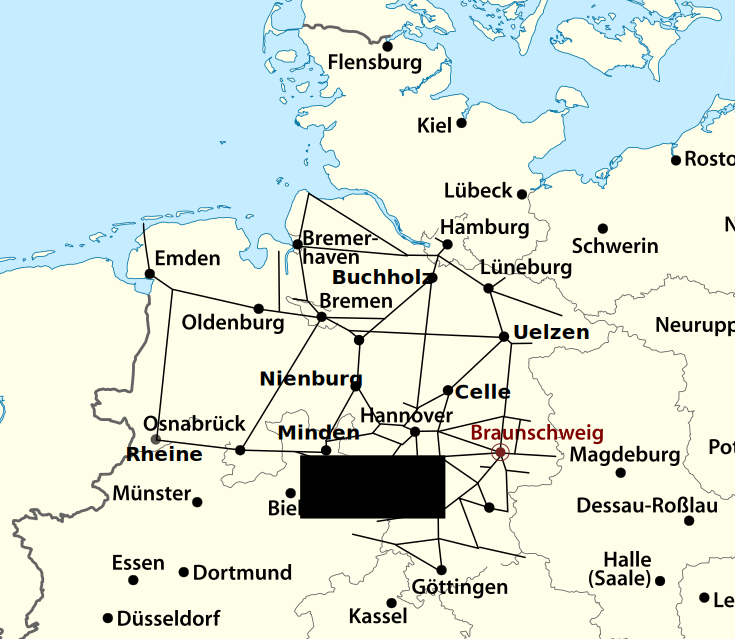
\includegraphics[width=\columnwidth]{bilder/ticket_deutschland.png}
\newpage
\includegraphics[width=\textwidth]{bilder/ticket_bis_11_Dezember.jpg}
\newpage
\input{texte/nuetzliches/streckenliste}

\begin{multicols}{2}
\subsection{Lernräume}
Hier fehlt noch Text, den man aber einfach von der fg-Seite nehmen kann.

\subsection{Exkursion zum 27C3}
Hier fehlt noch Text, den man aber einfach von der fg-Seite nehmen könnte, wenn denn dort mal was stünde.

\subsection{Ansprechpartner}
Hier fehlt noch Text, den man aber einfach von der fg-Seite nehmen kann.

% Dieser Trick hilft uns, eine neue Seite zu erzwingen
% (auf diese passt eh nix sinnvolles mehr) und dennoch die 
% Spaltenlängen auszubalancieren.
\end{multicols}

\includegraphics[angle=90,totalheight=\textheight, width=1.25\textwidth]
{texte/nuetzliches/stundenplan.pdf}
%  \end{multicols}
\newpage
\section{Sonstiges}

In diese Abschnitt %sollt ihr noch einmal zum Nachdenken angeregt werden,
bekommt eine "Ubersicht "uber das Semesterticket, % Hinweise zu eineranstehenden Exkursion,%
das Impressum, weitere Ansprechpartner neben der Fachgruppe, Campuskarten und euren Stundenplan.

\begin{multicols}{2}


\subsection{Ansprechpartner}
\paragraph{Fachgruppenrat}
%Zu Beginn des Semesters bietet die Fachgruppe wöchentlich einen Infotermin an - siehe Blog für die konkrete Zeit.

Im Normalfall treffen wir uns jede Woche zum Fachgruppentreffen
%Besprechung. Auch
Den  Termin entnehmt ihr bitte aus
\url{http://fginfo.cs.tu-bs.de/index.php/kontakt/fachgruppe/}.
\\\\
Beide Termine finden im Raum 149/150 des Informatikzentrums statt
(siehe dazu Seite \pageref{campuskarte}), in der vorlesungsfreien Zeit
jedoch nur nach Absprache. 
  Falls du eine Frage hast, kannst du gerne zum regulären
  Fachgruppentreffen kommen, oder einfach so mal vorbei schauen ob
  jemand da ist. Tipp: In der Stunde vor dem Treffen füllt sich der
  Raum schon langsam, also hast du da gute Chancen, Probleme in
  kleinerer Runde zu besprechen. 
 Ansonsten erreicht ihr uns natürlich via
Email unter \url{fginfo@tu-bs.de}.

\paragraph{Fachspezifisches}
Bei Fragen zu einem speziellen Fach auch der jeweilige Professor
bzw. Dozent - keiner von denen beißt! Am besten findet ihr die Profs
über die Seiten der jeweiligen Institute oder die Personensuche unter
\url{http://www.tu-braunschweig.de/suchoptionen/personen}.
%\paragraph{Weitere Ansprechpartner} 
%\begin{itemize}
\paragraph{\small Studiengangskoordinatorin} \ \\ Yvonne Sehnert ist die Studiengangskoordinatorin. Sie steht extra bereit,
um euch Fragen zu beantworten, und für alles, was sie nicht selbst
weiß, weiß sie, an wen Sie eure Frage weiterleiten muss.\\
{
Yvonne Sehnert\\
Carl-Friedrich-Gauß-Fakultät\\
Rebenring 58 A | Raum 124\\
Sprechzeiten: Nach  Vereinbarung\\
Telefon: (0531) 391-2843\\
E-Mail: \url{informatik-studium@tu-bs.de}
}

% \paragraph{\small Informatik Service-Desk}
% Heidi Schulze\\
% Informatikzentrum\\
% Mühlenpfordtstraße 23 | Raum G53\\
% Telefon: (0531)391-2116\\
% E-Mail: \url{schulze@cg.cs.tu-bs.de}\\
% \\
% Sprechzeiten: \\
% Mo. 10:00-12:00 Uhr
% \& 13:00-14:30 Uhr
% \\
% Do. 9:00-12:00 Uhr
% \& 13:00-16:30 Uhr
% %\end{itemize}
%\ \ \ \ \\ \\ \\ \\ \ \\
\paragraph{\small{Fachstudienberater}} \ \\
Dr. Werner Struckmann\\
Institut für Programmierung und Reaktive Systeme\\
Mühlenpfordtstraße 23 | Raum 244\\
Telefon: (0531) 391-3278\\
E-Mail: \url{struck@ips.cs.tu-bs.de}\\
\\
Sprechzeiten: Mi. 10:30-11:30 Uhr und nach  Vereinbarung

\paragraph{\small{Prüfungsamt}} \ \\
Rebecca Weidner\\
Carl-Friedrich-Gauß-Fakultät\\
Rebenring 58 A | Raum 127\\
Tel.: (0531) 391-2844\\
Fax: (0531) 391-8225\\
E-Mail: \url{pa-informatik@tu-braunschweig.de}\\
\\
Sprechzeit im Semester:\\
Di. und Do.:
9:30–12:00 Uhr und 14:00-16:30 Uhr\\
\\
Sprechzeit in der vorlesungsfreien Zeit:\\
Di. und Do.
9:30-12:00 Uhr \\


% Local Variables: 
% mode: latex
% TeX-master: "../../1-te"
% End: 


%\newpage \
\newpage
\subsection{Lernräume}
	Hier wollen wir euch eine aktuelle Übersicht über Lernräume an der TU Braunschweig geben. Die Liste ist im Moment nicht vollständig, sie wird aber demnächst erweitert und ist dann auf \url{http://fginfo.cs.tu-bs.de/index.php/studium/lernraume/} zu finden. Alle Gebäude stehen, wenn nicht anders in Anlage 1 der Hausordnung der TU Braunschweig erwähnt, von 7:30 bis 19:30 Uhr offen.
	\subsubsection*{Informatikzentrum}
		\begin{tabular}{|p{4cm}|p{4cm}|p{8cm}|}
			\hline Raum & Öffnungszeiten & Ausstattung \\ 
			\hline Plaza des Informatikzentrums & normal &  Tische und Stühle, Steckdosen unter Bodenabdeckungen zu finden \\
			\hline Fachgruppenraum der Informatik IZ 150 &
			nach Absprache mit Mitgliedern des
			Fachgruppenrates (wir ;) ) & Kaffemaschine, Sofas, Tische, Steckdosen in Massen sowie Ethernetkabel\\ 
			\hline Fachgruppenraum der Wirtschaftsinformatik
			IZ 159 & nach Absprache mit Mitgliedern des
			Fachgruppenrates Wirtschaftsinformatik (unsere
			netten Nachbarn :) )& Sofas, Tische und Steckdosen \\ 
			\hline CIP Pool IZ G40 & normal & Rechner-Pool mit Linux-PCs, Tafel\\ 
			\hline Gruppenarbeitsraum IZ 033 & normal &
			solange nicht anders belegt, Schlüssel gegen
			Pfand im Sekeratrat der Robotik bei Frau Engel,
			Raum G13 erhältlich.
			\hline
		\end{tabular}
	\subsubsection*{Andere Lernräume}
		\begin{tabular}{|p{4cm}|p{4cm}|p{3.6cm}|p{4cm}|}
 			\hline Raum & Öffnungszeiten & Ausstattung & Anmerkung  \\  
			\hline Grotrian  Zimmerstraße 24 & Normal  & Alte Tische und Stühle, vereinzelt Tafeln & Wenn Mitglieder der verschiedenen Fachgruppen anwesend sind hat das Grotrian meist länger offen. Da dies oft der Fall ist kann man hier meist lange lernen. \\ 
			\hline Bibliothek & Mo - Fr: 07:00 - 24:00 Sa: 10:00 - 20:00& Niedrige Tische und Stühle, Ruhezone, Rechnerarbeits\-plätze, Kopierer &  nicht zum  Lernen in der Gruppe  geeignet \\ 
			\hline Mensa / Cafeteria & Mo -Do: 08 - 20:00 Uhr Fr: 08:00 - 15:00 & Tische, Stühle, kein (!) WLAN, einzelner Rechner mit Netzzugang, Verpflegung incl. Selbstbedienungs-Kaffeeautomat& Probleme: Nicht durchgehend geöffnet, die Plätze sind primär zu Essen gedacht, von Lernsessions zu den Stoßzeiten sollte man also im eigenen und fremden Interesse absehen. \\ 
			\hline Bei dir zuhause & immer & Deine Sache & Achtung: Man lenkt sich leicht ab :) \\ 
			\hline Das eine oder andere Cafe / Kneipe & kommt drauf an & wechselhaft &Siehe die beiden vorherigen \\
			\hline
		\end{tabular}


\subsection{Campuskarte}
\label{campuskarte}
Bereits auf Seite \pageref{plan} habt ihr einen einfachen Campusplan
gesehen. Es gibt aber noch diverse andere Online:\\
Eine aktuelle Campuskarte, die durchsucht werden kann findet sich im
TUgether Portal unter \nurl{https://tugether.tu-braunschweig.de/}. Ihr
könnt euch dort mit eurer Y-Nummer einloggen.\\\\

Ein Raumplan für das 1. und 2. OG des Informatikzentrums findet sich
unter\\ \nurl{http://www.ibr.cs.tu-bs.de/rooms/rooms.html}
Sollten euch die genannten Links zu unhandlich zum Abtippen sein, findet ihr
auch alle unter
\nurl{http://fginfo.cs.tu-bs.de/index.php/studium/lernraume/}.
Dort findet ihr auch virtuelle Campustouren, die  in einem Web 2.0 Seminar entstanden und
bei Google Maps gehostet sind.
%ekeliger tabellenhack NICHT NACHMACHEN
%\begin{tabular}{c}
%\\  \\ \\ \\ \\ \\
%\end{tabular}

\end{multicols}
\vspace{5cm}
\newpage
\subsection{Impressum}
\label{impressum}
\begin{description}
\item[Herausgeber:]
	Fachgruppe Informatik\\
	c/o AStA der TU Braunschweig\\
	Katharinenstraße 1\\
	38106 Braunschweig\\
	Tel.: 0531/391-4569\\
	E-Mail: \url{fginfo@tu-bs.de}\\
	Webseite: \url{http://fginfo.cs.tu-bs.de/}
\item[V.i.S.d.P.:]  % Verantwortliche(r) im Sinne des Presserechts
  Lena Schimmel, Johannes Starosta
\end{description}
\begin{multicols}{2}
\begin{multicols}{2}
\subsection{Semesterticket}
	Euer Studentenausweis berechtigt euch zur Fahrt auf vielen Zugstrecken in Niedersachsen. Unten seht ihr den Gültigkeitsbereich des Semestertickets im Großraum Hannover. Nach Norden und und Westen deckt das Semesterticket weitere Strecken ab. Einen grober Überblick gibt die nebenstehende Karte. 

	Es d"urfen nur Regionalexpress (RE) und Regionalbahn (RB) der Deutschen Bahn AG, sowie teilweise der Metronom in der zweiten Klasse benutzt werden. Also NICHT Strecken der Nordwestbahn (NWB). Einen genauen Überblick findet ihr in Form einer Streckenliste auf der Seite \pageref{streckenliste1}.

	Mehr Details könnt ihr den Seiten des AStA unter \url{http://www.asta.tu-bs.de/semesterticket.php} bzw. \url{http://tinyurl.com/3gn8fhg} entnehmen.
\end{multicols}
\newpage
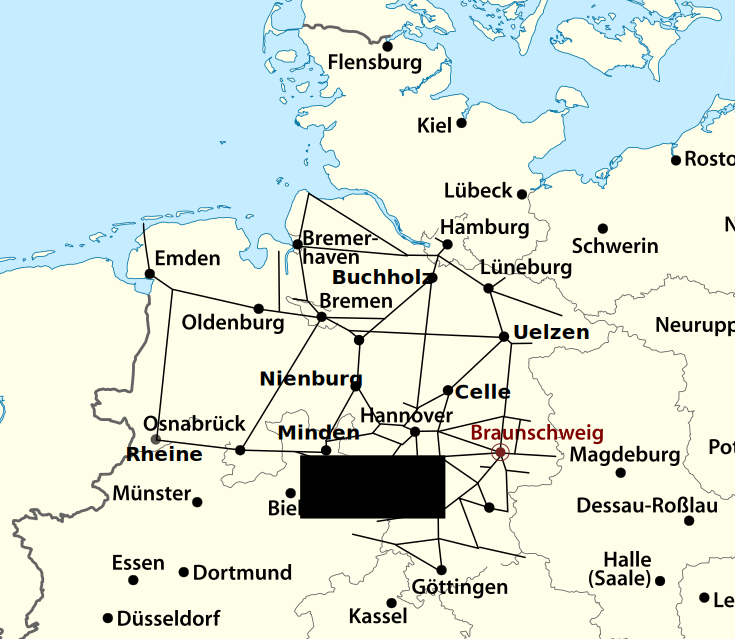
\includegraphics[width=\columnwidth]{bilder/ticket_deutschland.png}
\newpage
\includegraphics[width=\textwidth]{bilder/ticket_bis_11_Dezember.jpg}
\newpage
\input{texte/nuetzliches/streckenliste}
\end{multicols}

%\subsection{Exkursion zum 27C3}
Die Fachgruppe plant eine Exkursion zum 27C3. \\Dabei handelt es sich um
die diesjährige Ausgabe des Chaos Communication Congress des Chaos
Computer Clubs.\\ Die Exkursion wird aus
Studiengebühren finanziert. Aufgrund von Fristenvorgaben, muss die
Anmeldung bereits im Oktober erfolgen. Allerdings haben wir noch Plätze
für Selbstzahler. Außerdem springen immer mal wieder
Leute ab, weil sie dann doch keine Zeit haben. Das ist dann eure Chace
:)\\
Mehr Informationen findet ihr auf folgenden
Webseiten:\\
Zum Kongress selbst: \nurl{http://events.ccc.de/congress/}\\
Zur Exkursion: \nurl{http://fginfo.cs.tu-bs.de/index.php/tag/27c3/}

 %\newpage
%\nurl{http://maps.google.de/maps/ms?ie=UTF8&hl=de&msa=0&msid=110022173347618328583.00044f5213e3e4ab36c53&z=17}%\begin{multicols}{2}
%\hfill%\end{multicols}
%\begin{multicols}{2}
%Hier fehlt noch Text, Ein Raumplan für das 1. und 2. OG des Informatikzentrums findet sich unter http://www.ibr.cs.tu-bs.de/rooms/rooms.htmlden man aber einfach von der fg-Seite nehmen kann. Insbesondere geht's da um die Verweise auf die diversen Online-Karten wie er unter \url{http://fginfo.cs.tu-bs.de/index.php/studium/lernraume/} steht.

% Dieser Trick hilft uns, eine neue Seite zu erzwingen
% (auf diese passt eh nix sinnvolles mehr) und dennoch die 
% Spaltenlängen auszubalancieren.
%Hier fehlt noch Text, den man aber einfach von der fg-Seite
%nehmhttp://events.ccc.de/congress/en könnte, wenn denn dort mal was
%stünde.
\ifpdf
\newpage
\subsection*{Muster-Stundenplan Bachelor}
\includegraphics[angle=90,totalheight=0.95\textheight, width=1\textwidth]
{texte/nuetzliches/stundenplan.pdf}
\fi
%%% Local Variables: 
%%% mode: latex
%%% TeX-master: "../../1-te"
%%% End: 

  % der letzte der vorherigen Texte endet bereits einspaltig

  \end{multicols}

\end{document}
